%%
%% This is file `sample-authordraft.tex',
%% generated with the docstrip utility.
%%
%% The original source files were:
%%
%% samples.dtx  (with options: `authordraft')
%% 
%% IMPORTANT NOTICE:
%% 
%% For the copyright see the source file.
%% 
%% Any modified versions of this file must be renamed
%% with new filenames distinct from sample-authordraft.tex.
%% 
%% For distribution of the original source see the terms
%% for copying and modification in the file samples.dtx.
%% 
%% This generated file may be distributed as long as the
%% original source files, as listed above, are part of the
%% same distribution. (The sources need not necessarily be
%% in the same archive or directory.)
%%
%% The first command in your LaTeX source must be the \documentclass command.
\documentclass[sigconf,  % authordraft 
% nonacm
]{acmart}

\usepackage[T1]{fontenc}
%\usepackage{lmodern}
%\usepackage[utf8]{inputenc}
%\usepackage{amsfonts}
\usepackage{eurosym}
%\usepackage{amsmath}
%\usepackage{amssymb}
%\usepackage{booktabs}

%\usepackage{epsfig} 
%\usepackage{cite}
\usepackage{color}

% \usepackage{hyperref}

\usepackage[noend,ruled,vlined,linesnumbered]{algorithm2e}
\usepackage{multirow}
\usepackage{mathtools}
\usepackage{comment}
\usepackage{balance}

\usepackage{float}

%\usepackage{subfig}


    
% \usepackage[para]{footmisc}

\usepackage[inline]{enumitem}

\newtheorem{task}{Task}

% \setlength{\textfloatsep}{1.5em} 
% \setlength{\floatsep}{1.5em} 
% \setlength{\dbltextfloatsep}{1.5em}  % sep for 2-col-span floats

\newlength{\tsq}
\setlength{\tsq}{-1em}


\newcommand{\squishlist}{
 \begin{list}{$\bullet$}
  { \setlength{\itemsep}{0pt}
     \setlength{\parsep}{1pt}
     \setlength{\topsep}{1pt}
     \setlength{\partopsep}{0pt}
     \setlength{\leftmargin}{1em}
     \setlength{\labelwidth}{1em}
     \setlength{\labelsep}{0.5em} } }
 \newcommand{\squishend}{\end{list}}

\newcommand{\kp}[1]{\textit{\textcolor{violet}{KP: #1}}}
\newcommand{\GW}[1]{{\color{blue}GW: #1}}
\newif\ifdraft\drafttrue
\ifdraft
\newcommand{\todo}[1]{{\textcolor{red}{TH: #1}}}
\newcommand{\note}[1]{{\textcolor{red}{NOTE: #1}}}
\newcommand{\m}[1]{{\textcolor{red}{#1}}}
\else
\newcommand{\todo}[1]{}
\newcommand{\note}[1]{}
\fi

\newcommand{\sr}[1]{{\leavevmode\color{blue}SR: #1}}


%% \BibTeX command to typeset BibTeX logo in the docs
\AtBeginDocument{%
  \providecommand\BibTeX{{%
    \normalfont B\kern-0.5em{\scshape i\kern-0.25em b}\kern-0.8em\TeX}}}

%% Rights management information.  This information is sent to you
%% when you complete the rights form.  These commands have SAMPLE
%% values in them; it is your responsibility as an author to replace
%% the commands and values with those provided to you when you
%% complete the rights form.
\setcopyright{acmcopyright}
\copyrightyear{2021}
\acmYear{2021}
\acmDOI{xx.xxxx/xxxxxxx.xxxxxxx}

%% These commands are for a PROCEEDINGS abstract or paper.
\acmConference[WWW 2021]{The Web Conference}{April 19--23, 2021}{Ljubljana, Slovenia}
\acmBooktitle{WWW 2021: The Web Conference, April 19--23, 2021, Ljubljana, Slovenia}
% \acmConference[WSDM 2021]{ACM International WSDM Conference}{March 08--12, 2021}{Jerusalem, Israel}
% \acmBooktitle{WSDM 2021: ACM International WSDM Conference,
%   March 08--12, 2021, Jerusalem, Israel}
\acmPrice{15.00}
\acmISBN{[ISBN]}


%%
%% Submission ID.
%% Use this when submitting an article to a sponsored event. You'll
%% receive a unique submission ID from the organizers
%% of the event, and this ID should be used as the parameter to this command.
%%\acmSubmissionID{123-A56-BU3}

%%
%% The majority of ACM publications use numbered citations and
%% references.  The command \citestyle{authoryear} switches to the
%% "author year" style.
%%
%% If you are preparing content for an event
%% sponsored by ACM SIGGRAPH, you must use the "author year" style of
%% citations and references.
%% Uncommenting
%% the next command will enable that style.
%%\citestyle{acmauthoryear}

%%
%% end of the preamble, start of the body of the document source.
\begin{document}

%GW: no fiddling with style parameters
%%
%% The "title" command has an optional parameter,
%% allowing the author to define a "short title" to be used in page headers.
%\title[Searching for Entities with Numerical Constraint in Text]{Searching for Entities with Numerical Constraint in Text}
%\title[TabQs: Searching for Entities with Quantity Constraints from Quantitative Relational Web Tables]
%{TabQs: Searching for Entities with Quantity Constraints\\ from Quantitative Relational Web Tables}
\title{Extracting Contextualized Quantity Facts from Web Tables}
%%%GW: title should reflect the methodological contribution
%%%this paper should not be pitched as a system (demo) paper
%%%also de-emphasize query processing, as the novelty over ISWC 2019 paper is limited
%
%%
%% The "author" command and its associated commands are used to define
%% the authors and their affiliations.
%% Of note is the shared affiliation of the first two authors, and the
%% "authornote" and "authornotemark" commands
%% used to denote shared contribution to the research.
% \author{Anonymous Authors}
%  \email{anonymous@email}
%  \affiliation{
%       \institution{Anonymous Affiliation}
%   }

\author{Vinh Thinh Ho}
\email{hvthinh@mpi-inf.mpg.de}
\affiliation{
%  \institution{Max Planck Institute for Informatics}
   \institution{Max Planck Institut f\"ur Informatik}
 \city{Saarbr\"ucken}
 \country{Germany}
}

\author{Koninika Pal}
\email{kpal@mpi-inf.mpg.de}
\affiliation{%
    \institution{Max Planck Institut f\"ur Informatik}
 \city{Saarbr\"ucken}
 \country{Germany}
}

\author{Simon Razniewski}
\email{srazniew@mpi-inf.mpg.de}
\affiliation{%
   \institution{Max Planck Institut f\"ur Informatik}
 \city{Saarbr\"ucken}
 \country{Germany}
}

\author{Klaus Berberich}
\email{kberberi@mpi-inf.mpg.de}
\affiliation{%
   \institution{Max Planck Institut f\"ur Informatik}
     \institution{htw saar}
 \city{Saarbr\"ucken}
 \country{Germany}
}

\author{Gerhard Weikum}
\email{weikum@mpi-inf.mpg.de}
\affiliation{
   \institution{Max Planck Institut f\"ur Informatik}
 \city{Saarbr\"ucken}
 \country{Germany}
}


% \renewcommand{\shortauthors}{anonymous}

\begin{abstract}
%
%%%problem and what it involves
Quantity queries, with filter conditions on quantitative
measures of entities, are 
%so far out of reach 
beyond the functionality 
of search engines and QA assistants.
%%% not supported by search engines and QA assistants. 
%%% SR: "out of reach" brings imo out more that it is not just due to a lack of implementation, but due to missing methodology
To enable such queries over web contents,
this paper develops 
a novel
method for automatically extracting
quantity facts from ad-hoc web tables.
%%%GW: or should we say "the first method for ..."?
%%%SR: Yes I would say "the first" here - "a novel method for" sounds like there were already N works with similar output
This involves recognizing quantities, with normalized values and units,
aligning them with the proper entities, and contextualizing
these pairs with informative cues to match sophisticated queries with
modifiers. 
%
%%%approach and contribution
Our method
%method performs joint inference on entity linking and on
%%%GW: drop EL as a major contribution
 includes a new approach to aligning quantity columns
to 
%their respective 
entity columns.
%\color
%entity-quantity column alignment. 
%The latter was oversimplified in prior works
Prior works 
%by assuming 
assumed
a single subject-column per table,
whereas our approach is geared for complex tables and leverages
external corpora as evidence.
For contextualization, we identify informative cues from 
text and structural markup that surrounds a table.
For query-time fact ranking, we devise a new scoring technique that
exploits both context similarity and inter-fact consistency.
% SR: Expanded this point slightly
%technique for consistency corroboration.
%corroboration technique
%based on consistency learning.
Comparisons of our building blocks against state-of-the-art baselines
and extrinsic experiments with two query benchmarks demonstrate the 
benefits of our method.
%
\end{abstract}

\begin{comment}
\begin{abstract}
% below is old abstract
% Quantities appear in search queries in numerous forms: skyscrapers higher than 1000 ft, athletes who ran 200m under 20s, companies with annual profit above 10 billion USD, etc. Web tables are a rich source of information containing answers for this kind of queries.
% Modern search engines and QA systems
% can efficiently handle queries in the form of lookups (e.g., what is Bezos's net worth), which need to exploit only relational structures embedded in web tables for queried entities. But they fail to produce crisp answers to the queries involving quantity constraints as they disregard the reasoning over quantitative information.  
% In this paper, we develop a full-fledged QA system called TabQs that tackles queries with quantity constraints by harnessing quantitative  contextual information about entities presented in web tables. In particular, we propose a framework for extracting quantity facts from web tables, and a matching model to produce answers for given quantity queries. Experiments on real-world data demonstrate the effectiveness of our QA system on a set of benchmark questions, collected by crowdsourcing.


%%%problem and what it involves
Quantity queries, with filter conditions on quantitative
measures of entities, are so far out of reach of search engines and QA assistants.
%%% not supported by search engines and QA assistants. 
%%% SR: "out of reach" brings imo out more that it is not just due to a lack of implementation, but due to missing methodology
To enable such queries over web contents,
this paper develops a novel %the first 
method for automatically extracting
quantity facts from ad-hoc web tables.
%%%GW: or should we say "the first method for ..."?
%%%SR: Yes I would say "the first" here - "a novel method for" sounds like there were already N works with similar output
This involves recognizing quantities, with normalized values and units,
aligning them with the proper entities, and contextualizing
these pairs with informative cues to match sophisticated queries with
modifiers. 
%
%%%approach and contribution
Our method performs joint inference on entity linking and on
entity-quantity column alignment. The latter was oversimplified
in prior works by assuming a single subject-column per table,
whereas our approach is geared for complex tables and leverages
external corpora as evidence.
For contextualization, we identify informative cues from 
text and structural markup that surrounds a table.
For query-time fact ranking, we devise a new scoring technique that
exploits both context similarity, and inter-fact consistency.
% SR: Expanded this point slightly
%technique for consistency corroboration.
%corroboration technique
%based on consistency learning.
Comparisons of our building blocks against state-of-the-art baselines
and extrinsic experiments with a query benchmark demonstrate the 
%superiority
%advantages
benefits
of our method.


\end{abstract}
\end{comment}

%%
%% The code below is generated by the tool at http://dl.acm.org/ccs.cfm.
%% Please copy and paste the code instead of the example below.
%%
%\begin{CCSXML}
%<ccs2012>
% <concept>
%  <concept_id>10010520.10010553.10010562</concept_id>
%  <concept_desc>Computer systems organization~Embedded systems</concept_desc>
%  <concept_significance>500</concept_significance>
% </concept>
% <concept>
%  <concept_id>10010520.10010575.10010755</concept_id>
%  <concept_desc>Computer systems organization~Redundancy</concept_desc>
%  <concept_significance>300</concept_significance>
% </concept>
% <concept>
%  <concept_id>10010520.10010553.10010554</concept_id>
%  <concept_desc>Computer systems organization~Robotics</concept_desc>
%  <concept_significance>100</concept_significance>
% </concept>
% <concept>
%  <concept_id>10003033.10003083.10003095</concept_id>
%  <concept_desc>Networks~Network reliability</concept_desc>
%  <concept_significance>100</concept_significance>
% </concept>
%</ccs2012>
%\end{CCSXML}

%\ccsdesc[500]{Computer systems organization~Embedded systems}
%\ccsdesc[300]{Computer systems organization~Redundancy}
%\ccsdesc{Computer systems organization~Robotics}
%\ccsdesc[100]{Networks~Network reliability}

%%
%% Keywords. The author(s) should pick words that accurately describe
%% the work being presented. Separate the keywords with commas.

%\keywords{Semantic Search, Question Answering, Information Extraction,
%%Numeric 
%Quantities, Web Tables}
\keywords{Information Extraction, Quantity Facts, Web Tables}

%% A "teaser" image appears between the author and affiliation
%% information and the body of the document, and typically spans the
%% page.

%\begin{teaserfigure}
%  \includegraphics[width=\textwidth]{sampleteaser}
%  \caption{Seattle Mariners at Spring Training, 2010.}
%  \Description{Enjoying the baseball game from the third-base
%  seats. Ichiro Suzuki preparing to bat.}
%  \label{fig:teaser}
%\end{teaserfigure}

%%
%% This command processes the author and affiliation and title
%% information and builds the first part of the formatted document.

% \titlenote{This paper has been accepted at WWW 2021.}

\maketitle


%!TEX root = ../main.tex

\section{Introduction}\label{sec:intro}

\begin{comment}
\subsection{Contribution.}
The salient contributions of this work are as follows:
\begin{itemize}
\item We propose a joint model for entity disambiguation and quantity fact extraction in quantitative relational web tables.
\item We introduce TabQs, a system for answering quantity queries from web tables.
\item  We present extensive experiments on real-world data, showing the high quality of our approach.
\item A demo of our search system can be found at: \\ \textcolor{blue}{\url{http://tabqs-demo.webredirect.org/table/index.html}}
\end{itemize}
\end{comment}


%together with title, header, abstract should ideally end at end of first page 
%(with some leeway for spill-over)

\noindent{\bf Motivation.}
%
%
%quantity-centric queries, beyond lookups
%filters, comparisons, aggregates/rankings
%here: focus on quantity filters, as a building block
%give three examples
%simple
%- asian buildings/towers above/taller than 400 meters
%finance
%- football clubs worth more than 2 billion
%technology
%- mobile phones with battery capacity above 5000 mAh
%or tablets with ...
%- electric cars with energy consumption above 80 MPGe
%sports
%- sprinters who ran 100 meters under 9.9 seconds
%
%
A good fraction of web queries revolve around quantities of
entities: looking up, filtering, comparing and aggregating
quantitative properties such as heights of buildings, 
running times of athletes, goals or scoring rates of footballers,
energy consumption of electric cars, etc. 
\cite{DBLP:conf/semweb/HoIPBW19,DBLP:conf/wsdm/BondarenkoBVAFP20,DBLP:journals/corr/abs-2001-03272}.
In this paper we focus on {\em quantity filters}
\cite{DBLP:conf/semweb/HoIPBW19,DBLP:conf/wsdm/HoPKBW20}, 
%which are 
an important class
of queries and also a building block for comparative search.
Examples are:
\squishlist
%\item skyscrapers in Asia taller than 400 meters,
\item British football teams worth more than 1.5 billion pounds
\item sprinters who ran 100 m under 9.9 seconds
\item electric cars with energy efficiency above 80 MPG-e
\squishend


%point out that these are very different from lookups
%and that search engines and QA assistants don't handle them
Note that these are more difficult than quantity lookups,
such as 
%``the height of the Shanghai tower'' 
``the value of Manchester City''
or ``the 
personal 100 m record of Usain Bolt''.
Lookups are well supported by search engines and QA assistants.
Quantity filters, on the other hand, lack this support 
as conditions like ``more than 1.5 billion pounds'' or
``under 9.9 seconds'' are mostly interpreted in
string-matching mode. 
For some examples, search engines return good
web pages, such as Wikipedia articles on ``10-second barrier''
or ``100 metres'', but this is not the user's query intent
and she has to tediously sift through these pages rather
than receiving a crisp entity-list answer. 
Moreover, the result quality depends on the value in the query,
as some (string-interpreted) values match good list pages. For example, there is a list
of 100m races under 10 seconds, but none ready for 9.9, 9.8, etc.


%would be easy if KGs would have this data,
%or if one would know a specific high-quality DB (or web list/table) with the data
%alternatively, extract from a variety of highly heterogeneous sources
Instead of tapping the web, we could turn to knowledge bases (KBs)
and structured sources in the Open Data ecosystem. However, KBs
hardly cover quantities; for example, Wikidata contains thousands of
sprinters but knows their personal records only for a few instances.
To tap Open Data sources, one would still have to find the relevant datasets
in a sea of data sources, and assess their freshness and completeness.

\begin{table}[t]
\centering
\caption[]{
% Illustrative example on f
Football teams.}
\label{table:ExampleTable}
\vspace{\tsq}
{\footnotesize
\begin{tabular}{|l|l|l|l|l|}\hline
Team & Stadium & Capacity & Coach & Value (in Bio) \\ \hline
% Name & Site & Seats & Name & Value
% Team & Site & Seats & Team Mgr & Cost
Bayern & Allianz Arena & ca. 75000 & Hansi Flick &  2.549 Euro \\ 
% \hline
%https://www.forbes.com/teams/bayern-munich/
Real & Bernab\'{e}u & 81,044 & Zidane &  3.649 Euro \\ 
% \hline
%https://www.forbes.com/teams/real-madrid/#46086b336ed4
Man City & unknown & n/a & Pep Guardiola & 2.055 GBP \\ 
% \hline
Chelsea & Stamford Bridge & 40,834 & Frank Lampard & 1.958 GBP  \\ 
% \hline
%https://www.forbes.com/teams/chelsea/#38e1153c3725
Liverpool & Anfield & 53,394 & J\"urgen Klopp & ca. 1.7 GBP    \\ 
\hline
%Liverpool & Anfield & ??? & J\"urgen Klopp & ca. 1.7 GBP    \\ \hline
%https://www.forbes.com/teams/liverpool/#2c8bf1b46045

%https://www.forbes.com/soccer-valuations/list/#tab:overall
\end{tabular}
}%\small
	
\end{table}

%%%%%%%%%%%%%%%%%%%%%%%%%%%%%%%%%%%%%%%%%%%%%%%%%%%%%%%%%%%%%%%%%%%%%%%%
\vspace{0.1cm}
\noindent{\bf Problem.}
%
%quantity fact (fact, for short) extraction
%focus on web tables as input (as text was addressed in prior works)
%
At the core of answering quantity-filter queries is the problem of
extracting entity-quantity facts from web sources.
This has been successfully addressed in \cite{DBLP:conf/semweb/HoIPBW19} for
the case of single sentences from text sources, by recognizing entity-quantity pairs along with relevant context words and
 building on prior work for spotting quantities with numeric values
 and units \cite{DBLP:conf/kdd/SarawagiC14,DBLP:journals/tacl/RoyVR15,DBLP:conf/acl/SahaPM17}.
In this paper, we aim to tap into a different kind of data sources,
namely, ad-hoc {\em web tables} embedded in HTML pages, and address
the problem of accurately extracting entity-quantity facts with
relevant context. 
An {illustrative} example, 
%%%GW: good
which could serve to answer
the  query about British football teams, is shown in
Table \ref{table:ExampleTable}.


%involves the following steps, illustrated by example
%on first glance, prior works on web table extraction seems promising
%but ...
%point out the diffficulties
%
There are good prior works on extracting entity-centric facts from
web tables, including %\cite{DBLP:journals/pvldb/LimayeSC10,DBLP:conf/kdd/SarawagiC14,DBLP:journals/pvldb/VenetisHMPSWMW11,DBLP:journals/pvldb/CafarellaHLMYWW18,DBLP:journals/pvldb/LehmbergB17,DBLP:conf/edbt/OulabiB19,DBLP:conf/wims/LehmbergB19} and a recent survey \cite{DBLP:journals/tist/ZhangB20}. 
surveys 
\cite{DBLP:journals/pvldb/CafarellaHLMYWW18,DBLP:conf/acl/DongHLS20,DBLP:journals/tist/ZhangB20}.
The output is typically a set of
subject-predicate-object (SPO) triples, obtained by 
judiciously
picking two cells 
in the same row as S and O 
and deriving P from the column header of O. 
In conjunction with entity linking to a KG 
%\cite{DBLP:journals/pvldb/LimayeSC10,DBLP:conf/semweb/BhagavatulaND15,DBLP:conf/wims/RitzeLB15,DBLP:conf/cikm/IbrahimRW16,DBLP:conf/edbt/RitzeB17},
\cite{DBLP:journals/tkde/ShenWH15},
an extractor could yield, for instance, 
(\textit{Real Madrid, hasCoach, Zinedine Zidane}).

However, state-of-the-art methods do not work well for quantity facts
for several reasons:
\squishlist
\item First, quantities appear in very diverse and potentially noisy forms.
For example, the team values in Table \ref{table:ExampleTable} 
 are just strings,
varying in units and scale and missing values
(``unknown'', ``n/a'').
%in their units, and scale (billions) in the column header. Also values may be missing
%(unknown or n/a).
%Tables from web sites often pose even more difficult inputs.
Proper interpretation of table cells 
may require understanding the surrounding text.

%
\item Second, it can be hard to infer which column pair denotes a quantity fact,
that is, to which entity column a quantity column refers.
In the example Table \ref{table:ExampleTable}, we need to determine that Capacity refers to
Stadium and Value to Team, but this is not obvious for a machine.
This is further aggravated by the common situation that
column headers are more generic and less informative.
For example, instead of headers like Team, Stadium, Capacity, etc.
we could have Name, Site, Size, etc., which are hard
to interpret.
Prior works on web tables seemed to assume that all columns (for possible choices of O) refer
to the same column (for S), and that this per-row-entity column is usually
the leftmost one \cite{DBLP:journals/pvldb/CafarellaHLMYWW18, DBLP:journals/tist/ZhangB20}. However, these assumptions are not always true.
%
\item Third, extracting entity-quantity pairs alone is not sufficient
for query answering, as many queries include additional modifiers
such as ``British'' or cues for the measure of interest such as
``energy efficiency''. 
To be able to match these against a repository of quantity facts,
the fact extraction needs to capture also relevant context.
Prior works on triples from web tables ignored this important issue; they viewed the extraction as uncoupled from downstream use cases like user queries and questions. 
\squishend


%%%%%%%%%%%%%%%%%%%%%%%%%%%%%%%%%%%%%%%%%%%%%%%%%%%%%%%%%%%%%%%%%%%%%%%
\vspace{0.1cm}
\noindent{\bf Approach.}
%
%one short par, sketching the approach
%
This paper addresses the outlined problems and presents
a full-fledged solution, called {\bf QuTE} (\textbf{Qu}antity \textbf{T}able \textbf{E}xtraction), for extracting contextualized quantity facts
from web tables, to support quantity-filter queries. 
%%% now explain, in a nutshell, how we overcome each of the above three problems
%issue 1
First, to cope with noisy quantities and diverse units and scales in tables, we employ pattern-based extractors and 
rule-based normalization.
%issue 2
Second, for the problem of aligning the right pair
of entity and quantity columns, one of the key tasks, 
we devise a statistical inference method
that leverages external text corpora.
%We also revisit the entity linking, and 
%integrate it with the column alignment for
%joint inference.
%%issue 3
Third, to contextualize the extracted quantity facts,
we exploit text and DOM-tree markup that surround a table, and we introduce a novel way of computing confidence scores for quantity facts, based on evidence in text collections.
%
Finally, as the resulting facts may still yield
many 
false positives in query results,
we have developed additional methods for
enhanced scoring at query time
% , with external evidence from text and corroboration
based on consistency learning
\cite{DBLP:conf/mir/YagnikI07}.



%%%%%%%%%%%%%%%%%%%%%%%%%%%%%%%%%%%%%%%%%%%%%%%%%%%%%%%%%%%%%%%%%%%%%%%
\vspace{0.1cm}
\noindent{\bf Contribution.}
%
%one short par on contributions
%
%Our methodology includes the following novel contributions:
The following are novel contributions:
\squishlist
\item We present 
a robust solution for the 
column alignment problem posed by complex tables,
by harnessing external text corpora
and joint inference with entity linking.
This is the first method specifically geared for
extracting quantity facts, with the novel technique of
leveraging cues from a large text corpus (Sections \ref{sec:columnalignment}
and \ref{sec:qfact_scoring_model}).
%\kp{should we remove the word First here? making it slightly soft}
%\todo{not the first, but the first for quantity??}
%\GW{rephrased this}
\item We introduce a new way of computing quantity fact confidence scores, by incorporating evidence from text collection, with type-based inference to overcome sparseness problems (Section \ref{sec:qfact_scoring_model}).
\item We present a new method for corroborating
extracted facts at query time, re-ranking them and pruning false positives
based on a technique for consistency learning (Section \ref{sec:querying}).
%(originally devised for a different problem \cite{DBLP:conf/mir/YagnikI07}). 
%\cite{DBLP:conf/mir/YagnikI07}.
\item Experiments include comparative evaluations of
our major building blocks against 
%state-the-art 
various
baselines, and an extrinsic study of how well
the extracted facts support quantity queries.
The latter is based on a benchmark of 100 queries
from \cite{DBLP:conf/semweb/HoIPBW19} and a new
collection of 150 queries with list-based ground-truth.
\squishend
%\GW{we need to add the Qfact confidence scoring as a novel contribution, and clearly refer to Sections 4, 4 and 5.2 as our contributions -- this needs some further changes in the intro, will do later or tomorrow!}\\
%\GW{done}
% Experimental data and code are accessible at:\\
% URL
% \footnote{\textcolor{blue}{\url{URL}}}.
% \footnote{\url{URL}}.
% Experimental data, code and 
% a QuTE-based search demonstrator is available at \textcolor{blue}{\url{https://www.mpi-inf.mpg.de/research/quantity-search/quantity-table-extraction/}}
We make the experimental data and code available at 
\footnote{
% \textcolor{blue}{
~\url{https://www.mpi-inf.mpg.de/research/quantity-search/quantity-table-extraction}
% }
}.
A QuTE-based search demonstrator is accessible at
\footnote{
% \textcolor{blue}{
~\url{https://qsearch.mpi-inf.mpg.de/table/}
% }
}.



%!TEX root = ../main.tex

% \section{Computational Model and System Overview}
%\section{Problem Statement and Computational Model}
%\section{Computational Model and System Overview}
\section{Model and System Overview}
\label{sec:problem}
%In this section, we present the formal problem statement and important notations for our approach.
\label{sec:search}
\begin{figure*}[t]
% \vspace{-0.5em}

\centering
% \includegraphics[width=0.5\textwidth]{figures/ov3.pdf}
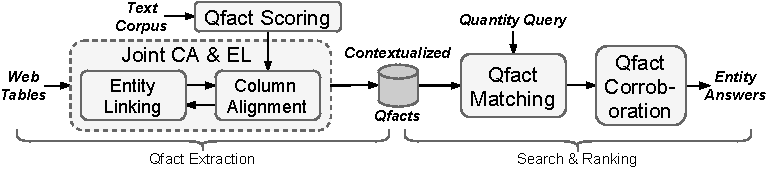
\includegraphics[width=0.7\textwidth]{figures/system_neu4}
% \includegraphics[width=0.75\textwidth]{figures/Qsearch-tables-architecture-11aug2020.pdf}
	\vspace{-0.5em}
\caption{Overview of the 
%Qtables 
QuTE
system.}
%  \vspace{-0.5em}
\label{fig:search_ov}
\end{figure*}

%\subsection{Problem Statement} 
%\noindent{\bf Model:}
\subsection{Model}
%The \textbf{input} of the problem is a \textit{quantity-filter} query (or quantity query) in the form of free text (e.g., 
%% \textit{``Hybrid cars with range on battery more than 50 miles''}, 
%\textit{``Stadiums with capacity more than 70k people''}
% , etc.
%), and a collection of relational web tables, where a relational table is defined as follows:
%GW: already covered in the intro
%
%%%GW introduce and define the key concepts
% web table, qfact, qquery and answer
%

The \textit{input} for fact extraction is a collection of
ad-hoc tables, from a web crawl, spreadsheet corpus
or Wikipedia dump
(e.g., \cite{DBLP:conf/bdc/EberiusBHTAL15}).

%\begin{definition}[Web Table]
\vspace{0.1cm}
\noindent{\bf Definition [Web Table].}
A web table with $r$ rows and
$c$ columns 
% consists of
is a tuple
% of $\mathcal{T} = (\mathcal{H},\mathcal{B}, \mathcal{X})$, where: \\
$T = (H, B, \mathcal{X})$ where:
\squishlist
%\item[-] $r$ and $c$ are two positive integers, denoting the number of rows and columns;
\item[-] ${H} = \{h_i | i \in \{1..c\}\}$ are the headers of the $c$ columns;
%where $h_i$ is the header of the $i$-th column;\\
\item[-] ${B} = \{b_{i,j} | i \in \{1..r\}, j \in \{1..c\}\}$ are cells in the table body;
%where $b_{i,j} $ denotes the cell at body row $i$ and column $j$; \\
\item[-] $\mathcal{X}$ is the context surrounding the table, which typically includes web page title, table caption, DOM-tree headings for the HTML path to the table,
and text in proximity to the table.
\squishend
% We denote $\mathcal{C}_k = \{h_k\} \cup \{b_{i,k} | i \in \{1..r\}\}$ as the $k$-th column of the table, consisting of a header $h_k$ and body cells $\{b_{i,k}\}$. 
% Moreover, we also denote $\mathcal{R}_k = \{b_{k,j} | j \in \{1..c\}\}$ as the $k$-th data row of the table.
We denote ${C}_k = \{h_k\} \cup \{b_{i,k} | i \in \{1..r\}\}$ and ${R}_k = \{b_{k,j} | j \in \{1..c\}\}$ as the $k$-th column and $k$-th row, respectively.
%\end{definition}

\vspace{0.1cm}
This definition is geared for ``horizontal'' tables with column headers and row-wise records. For ``vertical'' tables with row headers and data records per column, we can detect the orientation and apply a
{transpose} operation, using heuristics from \cite{DBLP:journals/pvldb/CafarellaHLMYWW18}.
%\todo{we need to remove "detect the orientation", so reviewers won't ask how to detect}
% \GW{keep this or drop the entire point?}
% \sr{Rewritten with reference I'd lean to keep it}

%Note that the above definition is for tables with horizontal header only (i.e., header is the first row instead of the first column). However, one can easily turn a table with vertical header into this format by using a \textit{``transpose''} operation. In the rest of the paper, we will only stick with this table format.

% \begin{example}
% Sample Table \ref{fig:preprocess_sample_1}-a has number of data rows $r = 4$; number of columns $c = 3$; headers $\mathcal{H} = \{h_1 : \textit{``Team''}, h_2 : \textit{``Stadium''}, h_3 : \textit{``Capacity''}\}$; body cells $b_{1,1} : \textit{``Marseille''}$, $b_{2,3}: \textit{``48,712''}$, etc.; and context caption $\mathcal{X} : \textit{``Stadiums with capacity''}$.
% \qed
% \end{example}

\vspace{0.1cm}
\noindent{\bf Definition [E-column and Q-column].}
For a given table, all columns whose cells 
predominantly contain named entities (which could be
linked to a knowledge base) are referred to as
E-columns. 
All columns whose cells predominantly contain
numeric quantities are denoted as Q-columns.
%
% \vspace{0.1cm}
The implementation of ``predominantly'' is
based on thresholds (say 80\%) for the
fraction of cells that qualify
one way or the other. 
Columns that are neither labeled E nor Q
(e.g., with many cells containing long text)
are disregarded.
%
In Table \ref{table:ExampleTable}, the columns
Team, Stadium and Coach are E-columns, and
Capacity and Value are Q-columns. 

\vspace{0.1cm}

The \textit{output} of extracting facts from a table is represented in the form of triples called 
{quantity facts}, or {\bf Qfacts} for short
(cf. \cite{DBLP:conf/semweb/HoIPBW19} where this terminology is
defined for text-based extraction).

\vspace{0.1cm}
\noindent{\bf Definition [Qfact].}
A quantity fact extracted from table
$T = (H, B, \mathcal{X})$ is a triple of the form
$\mathcal{F} = (e, q, X)$ where:
%%%GW: consider calling them EXQ triples, in contrast to SPO triples
\squishlist
\item[-] $e$ is an entity in a table-body cell $b_{i,j}$ of an
E-column $C_j$, either in the string form of an entity mention or already in the form of a linked entity
uniquely identified in a KB;
\item[-] $q$ is a quantity, properly normalized and with proper unit, in a cell $b_{i,k}$ of a Q-column $C_k$;
\item[-] $X$ is Qfact context, a (small) set of cue words 
(or phrases)
extracted from the table (incl. context $\mathcal{X}$)
that are specifically
informative for the pair $(e, q)$.
\squishend
\vspace{0.1cm}
As an example, a perfect extractor from Table \ref{table:ExampleTable} should produce Qfacts such
as 
(\textit{Estadio Santiago Bernab\'{e}u, 81044,
``stadium, capacity, seats, Madrid''}),
(\textit{Chelsea F.C., 1,958,000,000 GBP,
``team, value, football, London''}),
assuming informative text surrounding the table.

\vspace{0.1cm}
For the downstream use case of query answering, we consider a simple model of telegraphic or question-style
queries containing a single quantity filter,
following \cite{DBLP:conf/semweb/HoIPBW19}:

\vspace{0.1cm}
\noindent{\bf Definition [Qquery].}
A quantity query is a triple $\mathcal{Q} = (qt, qq, qX)$ where:
\squishlist
\item[-] $qt$ is the expected type of answer entities,
such as {\small\tt football team}
or {\small\tt sprinter};
\item[-] $qq$ is a quantity condition of the form ``$\theta ~\textit{value} ~\textit{unit}$'' where $\theta$ can be $\ge$, $\le$, between, or (approximately) equal,
and the unit is optional, as some measures do not have units, such as stadium capacity or country population;
\item[-] $qX$ is a set of additional qualifier terms
that an answer should match, such as ``British'' or ``100 meters'' or ``Olympics'', etc.
\squishend

\vspace{0.1cm}
The \textit{answer} to a Qquery is a Qfact that matches all query conditions, where context terms can be matched approximately (e.g., partially or by embedding-based
similarity):

\vspace{0.1cm}
\noindent{\bf Definition [Qanswer].}
An answer to a Qquery $\mathcal{Q} = (qt, qq, qX)$
is a Qfact $\mathcal{F} = (e, q, X)$ such that
$e$ is an entity of type $qt$,
$q$ satisfies the filter condition $qq$, and
$X$ is a sufficient match to the query context $qX$.
\vspace{0.1cm}

For example, the Qfact 
 (\textit{Chelsea F.C., 1,958,000,000 GBP,
``team, value, football, London''})
would approximately match a query about
``British football teams with value above 1.5 billion pounds'' (as ``British'' and ``London'' are highly
related by word embeddings).

\subsection{System}
%\kp{I changed the flow from here  till 3.4}


%All components of our approach, along with a quantity-query processor and
All components of QuTE, i.e, Qfact extraction method along with a quantity-query processor and
result ranker, are implemented in a 
pipeline depicted in Figure \ref{fig:search_ov}.
%We call our system {\bf QuTE} (for Quantity Table Extraction).
%pronounce: cute
%%%GW: may eventually rename into Qsearch-tables or so
%%%but here, we need to stay double-blind
%%%the name should emphasize the extraction, not the search (yet)

The pipeline starts with quantity recognition and
normalization for Q-columns and
entity linking to a KB for E-columns.
A crucial step then is 
column alignment that links a Q-column
with its proper E-column, to obtain a valid Qfact. %to align a Q-column with its proper E-column, to obtain a valid Qfact. 
%Entity linking and column alignment can be addressed
%by joint inference.
Contextualization and scoring of Qfacts involves
analyzing the 
context
% DOM tree and text 
around a table
and statistics from external corpora. Finally,
query processing involves matching and an additional
scoring step, taking inter-fact consistency into account.

%%%include table pre-processing already here
% For {\bf quantity recognition}, we employ a combination
% of the prior works on QEWT \cite{DBLP:conf/kdd/SarawagiC14} and 
% Illinois Quantifier \cite{DBLP:journals/tacl/RoyVR15}.
% The latter is used to extract numeric values and units from table cells. 
% QEWT is applied to the column headers to discover additional information about units and, possibly, scaling factors. Then, detected quantities are linked to the QuTree catalog~\cite{DBLP:conf/kdd/SarawagiC14} for normalization, including unit conversions.  

%\begin{comment}
%\GW{we have to keep this part, as it is a vital, albeit not original, building block; but we should go back to the previous version's concise text -- ToDo}\\
% \vspace{0.1cm}
% \noindent{\bf Quantity Recognition.}
%
%%%GW{this is old text not in the WSDM submission, which contains many English mistakes - dropped, went back to old WSDM text, don't edit this anymore!!!}
\begin{comment}
For \textbf{quantity recognition}, 
% We preprocess the input table to recognize quantities appearing in table's cells. 
unlike in text, where quantity value and unit go along each other, units of table quantities might appear in the Q-column header. 
Moreover, quantity value could 
% sometimes
be affected by a scaling factor (e.g., thousand, million), also given in the header.

% To recognize quantities in web tables, 
To tackle this,
we employ a combination
of the prior works on QEWT \cite{DBLP:conf/kdd/SarawagiC14} 
% -- providing a table column unit annotator based on a probabilistic context free grammar; 
and Illinois Quantitifer \cite{DBLP:journals/tacl/RoyVR15}.
% -- a tool for extracting quantity from text. 
The latter is used to extract numeric values and units from table body cells $b_{i,j}$. QEWT is applied to the column headers $h_i$ to discover additional information about units and, possibly, scaling factors. 
% If both the header and the body cell provide quantity units, we prioritize using the one given in the header (detected by QEWT), as we observed that units of body cells given by Illinois Quantitier are more noisy.
Then, detected quantities are linked to the QuTree catalog~\cite{DBLP:conf/kdd/SarawagiC14} for normalization, including unit conversions. 
\end{comment}
%
% Detected quantities are linked to the QuTree unit catalog \cite{DBLP:conf/kdd/SarawagiC14}, which provides various units and conversion factors over different measurements, so that they are comparable.

%The latter uses rules to extract numeric values and units
%from table cells. QEWT is applied to the column headers to discover additional information about units and,
%possibly, scaling factors. 
%For normalization, including unit conversions,
%we link detected quantities to the QuTree catalog of
%\cite{DBLP:conf/kdd/SarawagiC14}.
% , that enables comparison between quantities.


%%%GW: here is the polished text from the WSDM submission - fully sufficient!

For {\bf quantity recognition}, we employ a combination
of the prior works on QEWT \cite{DBLP:conf/kdd/SarawagiC14} and 
Illinois Quantifier \cite{DBLP:journals/tacl/RoyVR15}.
The latter is used to extract numeric values and units from table cells. 
QEWT is applied to the column headers to discover additional information about units and, possibly, scaling factors. Then, detected quantities are linked to the QuTree catalog~\cite{DBLP:conf/kdd/SarawagiC14} for normalization, including unit conversions.  

% \vspace{0.1cm}
% \noindent{\bf Entity Recognition.}
For \textbf{entity recognition}, 
% To recognize entities from table body cells $b_{i,j}$,
we employ the
% Stanford NER tool 
% ({\small\url{https://nlp.stanford.edu/software/}})
% and 
AIDA dictionary (\textit{\url{github.com/ambiverse-nlu}}), which provides a large set of entity 
%mentions
names,
such as ``Real'', ``Bayern'', etc.,
and candidate entities.
%along with their candidate entities based on name matches and string similarity, 
%e.g., ``Bayern'':
%{\it Bayern (song)}, 
%{\it Bavaria (Germany)}, 
%{\it FC Bayern Munich}, 
%etc.
%Their disambiguation via entity linking is discussed in Section \ref{sec:extract}.

%\GW{now add a short par on EL here}\\
For {\bf entity linking (EL)} (i.e., disambiguating the recognized mentions onto KB items), there are ample prior works specifically geared for web tables 
\cite{DBLP:journals/pvldb/LimayeSC10, DBLP:conf/semweb/BhagavatulaND15, DBLP:conf/cikm/IbrahimRW16, DBLP:conf/semweb/EfthymiouHRC17, DBLP:conf/edbt/RitzeB17}. We 
%mostly
follow 
\cite{DBLP:conf/semweb/BhagavatulaND15}, with inference
over a probabilistic graphical model. This takes into account a prior for entity popularity, 
context similarity between mentions in table cells and the KB entities, and the coherence among entity candidates for the same row (which should be semantically related entities) and the same column (which should be of the same semantic type). We denote result entities by $\Phi$, with $\Phi(b_{i,j})$ is the entity for input mention $b_{i,j}$ in the table body. 
% For input mentions $b_{ij}$ in the table body, we denote the resulting entities by $\Phi(b_{i,j})$.


%Based on the above steps and using thresholds for
%the per-column fractions, we mark each column either as an {\bf E-column} or a {\bf Q-column} (or as ``none'' in some exceptional cases).
%GW: already said earlier, would be repetition here



%!TEX root = ../main.tex

%\section{QFact Extraction From Web Tables}
%\section{Entity Linking \& Column Alignment}}
%\label{sec:extract}

\begin{comment}
In this section, we describe our method for extracting Qfacts from web tables, which is done in a quantity-centric manner. For each quantity of the input table, we find the entity to which it refers, and the context tokens that express the their relation. 
We rely on the following characteristics of relational tables for extracting Qfacts:
\squishlist
\item First, each quantity and its referred entity are on the same row.
\item Second, quantities of the same column refer to entities of the same column.
\item Third, quantities of the same column refer to (mostly) the same context, which is mainly expressed by the column header, might including some external cues from the table context. Note that contexts of quantities on the same column might slightly differ as they could also be affected by other tokens of the same row.
\squishend
% We rely on the following four assumptions for extracting Qfacts:
% \begin{itemize}
% \item First, each quantity carries information about only one entity in the table. 
%  \sr{so a table showing for all pairs of clubs how they played against each other would be out of scope - this excluded case seems more important to mention to me than unions of entities. In comparison, the other assumptions below look like trivialities to me.}
% \item Second, each quantity and its referred entity should be in the same row.
% \item Third, quantities of the same column refer to entities of the same column.
% \item Finally, quantities of the same column refer to the same context.
% \end{itemize}
% \noindent These assumptions reflect the nature of relational table structure. Unlike in natural text, where quantity might contains information about more than one entity (e.g., \textit{``China and India currently account for about 37\% of the entire global population''} -- the quantity 37\% refers to both China and India), the structure of tables implies the isolation of information between data rows (i.e. removing one row does not affect the understanding of other rows), and each column usually represents additional information for another one, which is especially frequent in case the column is quantity. The relation between each two cells on the same row of the connected entity-quantity columns are usually the same, where its meaning is mainly expressed by the headers, might including some external cues from the table context. One example of table that breaks these assumptions is when one cell contains more than one entity (e.g., \textit{``China \& India''} both in one cell). However, this kind of table is infrequent and hence we do not support.
%(we mark these cells as \textit{none} instead of dropping the whole table).

% \noindent These assumptions reflect the nature of relational table structure. Unlike in natural text, where quantity might contains information about more than one entity (e.g., \textit{``China and India currently account for about 37\% of the entire global population''} -- the quantity 37\% refers to both China and India), the structure of tables implies the isolation of information between data rows (i.e. removing one row does not affect the understanding of other rows), and each column usually represents additional information for another one, which is especially frequent in case the column is quantity. The relation between each two cells on the same row of the connected entity-quantity columns are usually the same, where its meaning is mainly expressed by the headers, might including some external cues from the table context. One example of table that breaks these assumptions is when one cell contains more than one entity (e.g., \textit{``China \& India''} both in one cell). However, this kind of table is infrequent and hence we do not support.


\noindent With these characteristics, the Qfacts extraction task is turned into a column alignment problem. In particular, for each quantity column of the input table, we want to find an entity column to which it refers and the context that expresses their relation. Below, we describe in detail our approach for extracting Qfacts from tables, which consists of two main phases: \textit{Preprocessing} and \textit{Column Alignment}.


\subsection{Table Preprocessing}
In this phase, we preprocess each input table by detecting quantities and entity candidates appearing in table's cells. Given raw input table $\mathcal{T} = (r, c, \mathcal{H},\mathcal{B}, \mathcal{X})$, we preprocess $\mathcal{T}$ by the following steps:

\begin{table}[t]
\centering
\caption{Football teams \textnormal{\textit{(preprocessed)}}.}
\label{table:ExampleTablePreprocessed}
\vspace{-1em}
\setlength{\tabcolsep}{0.34em}
{\footnotesize
\begin{tabular}{l|l|l|l|l}
\multicolumn{5}{l}{\textit{Entity columns: (\#);\ \ \ \ Quantity columns: (*)}}\\
\hline
\textit{(\#)} Team & \textit{(\#)} Stadium & \textit{(*)} Capacity & \textit{(\#)} Coach & \textit{(*)} Value (in Bio) \\ \hline
% Name & Site & Seats & Name & Value
% Team & Site & Seats & Team Mgr & Cost
``Bayern'' & ``Allianz Arena'' & (75000;) & ``Hansi Flick'' &  (2.549e9; \euro) \\ 
% \hline
%https://www.forbes.com/teams/bayern-munich/
``Real'' & ``Bernabeu'' & (81044;) & ``Zidane'' &  (3.649e9; \euro) \\ 
% \hline
%https://www.forbes.com/teams/real-madrid/#46086b336ed4
``Man City'' & unknown & n/a & ``Pep Guardiola'' & (2.055e9; \pounds) \\ 
% \hline
``Chelsea'' & ``Stamford Bridge'' & (40834;) & ``Frank Lampard'' & (1.958e9; \pounds)  \\ 
% \hline
%https://www.forbes.com/teams/chelsea/#38e1153c3725
``Liverpool'' & ``Anfield'' & (53394;) & ``J\"urgen Klopp'' & (1.7e9; \pounds)    \\ 
\hline
%Liverpool & Anfield & ??? & J\"urgen Klopp & ca. 1.7 GBP    \\ \hline
%https://www.forbes.com/teams/liverpool/#2c8bf1b46045

%https://www.forbes.com/soccer-valuations/list/#tab:overall
\end{tabular}
}
		
\end{table}

\vspace{0.1cm}
\noindent \textbf{Recognizing Quantities.}
We pre-process the input table to recognize quantities appearing in table's cells. Unlike in text, where the quantity value and unit go along each other, unit of table quantities might appear in the column header. Moreover, the numeric values in the column body could sometimes
% sometimes do not represent quantity values, because they are 
be affected by a multiplier (e.g., thousand, million), which also appears in the header .

To recognize quantities in web tables, we use a combination of the two previous works: QEWT \cite{DBLP:conf/kdd/SarawagiC14} -- providing a table column unit annotator based on a probabilistic context free grammar; and Illinois Quantitifer \cite{DBLP:journals/tacl/RoyVR15} -- a tool for extracting quantity from text. We apply the Illinois Quantitifer on each individual body cell $b_{i,j}$ of the input table to detect quantity value and unit (if available). We also run QEWT on each table header $h_k$ to detect a unit and (optional) a multiplier, which apply for its corresponding column. The quantity values in body cells are multiplied with the multiplier if it is available. Moreover, if both the header and the body cell provide quantity units, we prioritize using the one given in the header (detected by QEWT), as we observed that units of body cells given by Illinois Quantitier are more noisy. Detected quantities are linked to the QuTree unit catalog \cite{DBLP:conf/kdd/SarawagiC14}, which provides various units and conversion factors over different measurements, so that they are comparable.

\vspace{0.1cm}
\noindent \textbf{Detecting Entity Candidates.} 
In this step, we detect entity mentions in table cells. For each mention, we find a set of candidate knowledge base entities that it could link to, which will be disambiguated later. For each cell $b_{i,j}$ of the input table with text content $t$, we identify a potential mention $m$ as the longest substring of $t$ that has non-zero probability $P(e|m) > 0$ for some entity $e$. The set of candidate entities $C(m)$ for the mention $m$ is determined as all those $e$, i.e., $C(m) = \{e|P(e|m) > 0\}$.
\begin{example}
With $m =\textit{``Bayern''}$, $C(m)$ includes: 
\textit{<KB:Bayern\_(song)>}, 
\textit{<KB:Bavaria\_(Germany)>},  
\textit{<KB:FC\_Bayern\_Munich>},
etc.
\qed
\end{example}
We pre-compute the prior probability $P(e|m)$ for entities of the YAGO knowledge base \cite{DBLP:conf/www/SuchanekKW07} from hyperlinks in two corpora: Wikilinks \cite{singh2012wikilinks} and Wikipedia.
% (both text + tables).

\vspace{0.1cm}
\noindent \textbf{Annotating Columns.}
Based on the quantities and entity candidates annotations, we assign each cell $b_{i,j} \in \mathcal{B}$ as either \textit{entity-cell}, \textit{quantity-cell}  or \textit{none-cell} (if it does not contain entity or quantity, or we cannot recognize them).
%In case a cell contains both entity and quantity, we assign them as \textit{none-cell}.
Then, we mark each column of the table as either \textit{quantity-column} or \textit{entity-column}, based on the majority of quantity or entity mentions from the column's cells.  
Tables \ref{table:ExampleTablePreprocessed} shows an example of this preprocessing step.


%or \textit{none-column}. In particular, we label a column as \textit{quantity-column} if at least 50\% of its body cells are \textit{quantity}, \textit{entity-column} if at least 50\% of its body cells are \textit{entity}, and \textit{none-column} otherwise.

%%%%%%%%%%%%%%%%%%%%%%%%%%%%%%%%%%%%%%%%%%%%%%%
 
\subsection{Entity Linking (EL)}
\label{subsec:EL}

%\begin{definition}[Entity Assignment] 
\noindent{\bf Definition [Entity Assignment].} 
Given a preprocessed table ${T}$ with 
a set of 
entity mentions $\{m_1, m_2, ...\}$, an entity assignment $\Phi$ is a 
% (possibly partial)
mapping of mentions onto entities in a KB:
$\Phi: m_i \rightarrow e_i \in \mathcal{C}(m_i)$
where $\mathcal{C}(m_i)$ is the set of candidate entities for $m_i$.
%Putting into words, for entity linking, we want to choose the right entity for each mention that best interprets the table.
%\end{definition}
\vspace{0.1cm}

There is ample prior work on entity linking for web tables (e.g., \cite{DBLP:journals/pvldb/LimayeSC10, DBLP:conf/semweb/BhagavatulaND15, DBLP:conf/cikm/IbrahimRW16, DBLP:conf/semweb/EfthymiouHRC17, DBLP:conf/edbt/RitzeB17}). We mostly follow 
\cite{DBLP:conf/semweb/BhagavatulaND15}, 
%but devise an important extension.
with an extension regarding entity types.
% The $\textit{homogeneity}(\theta)$ score reflects the coherence of each candidate entity in $\theta$ with the table context and other candidate entities. The green lines in Figure \ref{fig:scoring} depict these entity connections.
% In this work, we adopt Markov Random Fields, which have been successfully employed for entity disambiguation in web tables by previous works \cite{DBLP:conf/semweb/BhagavatulaND15, DBLP:conf/cikm/IbrahimRW16}. Our graphical model is a light-weight modified version from these works.
%, where we restrict potential functions to contain entity variables within the same column.
{\color{blue}
This method adopts Markov Random Fields, presents the table's entity mentions as a set of variables $H = \langle E_1, E_2, ... E_k \rangle$ where $E_i$ refers to the target entity of mention $m_i$ of the table. The MRF defines a set of potential functions $\Psi$ that capture the relationships between these variables; and then represents the joint probability distribution of $H$ as follows:
%\[
%\textit{h\_score}(\mathcal{C}_v|\theta) = \textit{Pr}(H_v[\theta]) = Z^{-1}\prod_{f \in F_\Phi}\Phi_f
% \]
\[
\textit{EL-score}(\Phi) = \textit{Pr}(H[\Phi]) = Z^{-1}\prod_{f \in F_\Psi}\Psi_f
 \]
where $H[\Phi]$ is a realization of $H$ based on entity  assignment $\Phi$,
 $F_\Psi$ is the set of $H$'s variable subsets over which $\Psi$ is defined, and $Z$ is a scaling factor to give the true probabilities. For simplicity, we omit $Z$ and use a log-likelihood version when computing \textit{EL-score}.
 }
 For defining potential functions $\Psi$, 
%  following previous works \cite{DBLP:conf/semweb/BhagavatulaND15, DBLP:conf/cikm/IbrahimRW16}, we restrict to use edge-observation and node-observation features only. In our work, we modelize the joint distribution $\textit{Pr}(H)$ using the following features:
the following signals are combined into the graphical model:
 
% This method combines the following signals into
% a probabilistic graphical model:
\squishlist
\item {\em Prior probability:} the likelihood that an entity is mentioned, estimated from popularity statistics (e.g., Wikipedia page visits or article lengths)
and frequencies of href anchors.
\item {\em Context similarity:}
the degree of the context of mention $m$ in table cell $b_{i,j}$ matching the description of candidate entity $e$ (e.g., by
Wikipedia excerpts 
on $e$ 
or derived embeddings).
The context of $b_{i,j}$ comprises table header $H$, row $R_i$,
column $C_j$ and table context
$\mathcal{X}$ (caption, page title, etc.).
\item {\em Row-wise coherence:} 
mentions that appear in the same row 
$b_{i,*}$ should be mapped to 
semantically related entities, with relatedness
from Wikipedia signals (e.g., inlink overlap)
or embedding-based distance.
\item {\em Column-wise coherence:} 
mentions in the same column $b_{*,j}$
should be mapped to semantically related entities.
\squishend
We construct the graphical model from these constituents
% we construct a 
%Markov Random Field (MRF) and perform Monte Carlo sampling to
% graphical model and
and approximate the best entity assignment $\Phi$,
% which maximizes $\textit{EL-score}(\Phi)$, 
similar to
\cite{DBLP:conf/semweb/BhagavatulaND15}.
% The random variables are all mentions, with entities as values, and the factors 
%(potential functions)
% couple random variables by the above constituents.

%\GW{so far, we follow the literature; next we present our extension on homogeneity}

\todo{maybe remove the type agreement below}

Our extension of this method builds on the hypothesis that all (or most) entities in the same column should share an informative semantic type, such as 
{\small\tt football team} or {\small\tt sports arena}.
This can be seen as refinement of the factors for per-column coherence, but it also relaxes the
relatedness between same-column mentions and
solely focuses on the type cues.

We can easily find high-level common types
such as {\small\tt organization}
or {\small\tt person}.
These are insufficient signals, though.
We aim to identify 
a specific type 
%(in the knowledge base)
that the mentions in the same column 
could
potentially have in common
(for some choice of entity candidates).

\vspace{0.1cm}
\noindent{\bf Definition [Type Agreement].}
Given two entities $e_i$ and $e_j$, their agreement is computed from their
most specific common type $t$ as follows:
% \vspace{0.1cm}
\[
\textit{agree}(e_i, e_j) = \max\big(\textit{itp}(t)\ |\ t \in \textit{types}(e_i) \cap \textit{types}(e_j)\big)
\]
% \vspace{0.1cm}
\noindent where $\textit{types}(e_i)$ is the set of all types for $e_i$ obtained from the KB 
(using YAGO, {\small\tt yago-knowledge.org}, as it has an expressive type system) 
and $\textit{itp(t)}$ (\textit{inverse type population}) denotes the specificity of $t$, 
%from the total number of KB entities having type $t$ as:
defined as:
$$\textit{itp}(t) = \log_{10}\bigg(\frac{\#\textit{total\_kb\_entities - \#\textit{entities\_with\_type\_t} ~+~ 0.5}}{\#\textit{entities\_with\_type\_t} ~+~ 0.5}\bigg)$$
% We compute global values for \textit{itp} from type information of all entities in YAGO, 

\noindent \textit{itp} is analogous to \textit{inverse document frequency (idf)}. Types with a low number of entities in the KB are most informative.
%\textit{itp} value, and vice versa.
%
%We could apply this computation of most specific type to all mentions in the same column
%(generalizing the above definition from pairs to 
%entire sets), and enforce a threshold of
%type agreement among a fraction of the column cells.
%However, we do not need to enforce such a
%restrictive constraint. 
%
%GW: added this high relevance of Limaye et al.
%This resembles considerations in \cite{DBLP:journals/pvldb/LimayeSC10}.
%However, this prior work enforced a hard constraint,
%computing the per-column most specific common type upfront, and then restricting the EL to entities of that type.
%GW: no true, Limaye et al just use types as features/factors
%Instead, 
We treat
the type agreement between a pair of same-column cells
as another factor that is included into 
the collective inference.
\end{comment}

%%%%%%%%%%%%%%%%%%%%%%%%%%%%%%%%%%%%%%%%%%%%%%%

\section{Column Alignment}
\label{sec:columnalignment}


%\todo{I suggest to change the section title to "Quantity Column Alignment" to focus on quantity}

%The QuTE system build upon the column alignment task. 
%In this section, we discuss the weaknesses in existing quantity column alignment approach and propose a robust method to handle them.  
A major building block of QuTE is the column alignment, which aligns a Q-column with its proper E-column, in order to extract Qfacts from the right pair of columns. This section discusses the limitation of prior works on web table processing and proposes a robust method for this task.
Key novelties of our method are to leverage cues from an external text corpus, and to couple the inference for column alignments with the entity linker.

\vspace{0.1cm}
\noindent{\bf Definition [Column Alignment (CA)].}\\
%\begin{definition}[Column Alignment] 
Given a pre-processed table ${T}$ with $x$ Q-columns $\{{C}_{k_1},{C}_{k_2},..., {C}_{k_x}\}$ and $y$ E-columns $\{{C}_{v_1},{C}_{v_2},..., {C}_{v_y} \}$, a column alignment is a function $\Lambda$ that maps each Q-column to one E-column:\\
$\Lambda = \big\{{C}_{k_i} \rightarrow {C}_{v_j}|~i \in \{1..x\}\big\}$
%\end{definition}
%\vspace{0.1cm}

\subsection{Heuristics and their Limitations}
\label{subsec:CA-priorworks}

%GW: now discuss basic CA methods, as baselines
Column alignment has been addressed in prior works 
\cite{DBLP:journals/pvldb/VenetisHMPSWMW11,DBLP:journals/pvldb/DengJLLY13,DBLP:conf/er/BraunschweigTL15}
 under simplifying assumptions, like
mapping all Q-columns to the same E-column,
which boils down to identifying a single
subject column for the entire table.
We overcome this limitation, but nevertheless
consider heuristics that are inspired from prior works.

%\todo{emphasize that there are related works that do not link all O-col to a single S-col, however non of them work for quantity}

\vspace{0.1cm}
\noindent{\bf Definition [Leftmost Heuristic].}
Each Q-column $C_k$ is mapped to the leftmost
E-column $C_v$, that is, the smallest $v$
for which $C_v$ qualifies as an E-column.

\vspace{0.1cm}
\noindent{\bf Definition [Closest-Left Heuristic].}
Each Q-column $C_k$ is mapped to the closest
E-column $C_v$ that is left of $C_k$, that is,
$v < k$ and $k-v$ is minimal.

\vspace{0.1cm}
\noindent{\bf Definition [Most-Unique Heuristic].}
Each Q-column is mapped to the 
E-column with the largest number of unique values
(resembling a relational key).
In case of a tie, 
% one of the other heuristics serves as tie-breaker.
pick the leftmost one.
\vspace{0.1cm}

%%%motivate and highlight our novel contribution
In many cases, these three heuristics perform remarkably well,
notwithstanding their simplicity.
For our example in Table \ref{table:ExampleTable},
they would be far from perfect, though.
The Leftmost heuristic maps all Q-columns to
Team. 
%It would be able, though, to skip even more leftmost columns with numbers such as ranks, which are common in web tables.
The Closest-Left heuristic correctly aligns
Capacity to Stadium, but erroneously 
aligns Value to Coach.
The Most-Unique heuristic does not help in
this example, as all table cells have unique values.

%%%GW: new text here
Methods that consider multiple subject columns within the same table mostly rely on linking column headers to classes or concepts in a comprehensive knowledge base (e.g., \cite{DBLP:journals/pvldb/LimayeSC10, DBLP:conf/semweb/BhagavatulaND15, DBLP:conf/cikm/IbrahimRW16, DBLP:conf/semweb/EfthymiouHRC17, DBLP:conf/edbt/RitzeB17}), to map column pairs to KB relations. However, quantity measures are covered only very sparsely in state-of-the-art KBs.
As our goal is to cover a wide variety of 
%quantities and their respective entity types,
quantity types,
we cannot 
% do not want to 
%make this strong assumption, as KBs hardly cover quantities. 
rely on the KB for column alignment.
%Instead, we just align two columns directly, without any need for a KB. \todo{we still use KB actually, for entity linking + type-lifted traversal, need to make this statement soft, or remove}
%\GW{rephrase - I think it is now proper wording}
The only prior work for handling multiple subject columns and aligning other columns without assuming a prior KB
is \cite{DBLP:conf/er/BraunschweigTL15}.
%(\todo{'only' sounds very strong, I think there are works that map column pairs to KBs relation, but they also don't work for quantity (we actually mentioned this in Sec 3.2: 'Prior work on extracting SPO triples from web tables often re-sorted to pre-existing triples in a knowledge base as 'witness'...), I think we should remove 'only'})\kp{'only' is fine here. I would rather prefer not to bring up the prior works for aligning pair of E-columns to avoid confusion.}
%
This method is based on discovering functional dependencies by 
analyzing entropy measures between columns. However, in Q-columns the
typical situation is that all values are distinct, so that their frequencies
are trivial and do not give hints for cross-column scoring.
Moreover, we found that even when a web table has multiple E-columns,
the values in all of them are often unique -- as tables often
have only few rows. Table \ref{table:ExampleTable} is a typical case,
and the method of \cite{DBLP:conf/er/BraunschweigTL15} does not 
add any benefit over the simpler heuristics here.
Hence we disregard this method.

%%%%%%%%%%%%%%%%%%%%%%%%

\begin{comment}

To overcome the drawback in heuristic-based methods, we propose a graph-based
approach to aligning a Q-column to its E-column. Our proposed column alignment
method requires two preprocessing steps-- 1) detection of Q-column and E-column
and 2) an initial entity linking for E-column. We first present these
preprocessing steps before jumping to the explanation of our proposed column alignment method.

\subsection{Detection of quantity and Entity column}
For \textbf{quantity recognition}, 
unlike in text, where quantity value and unit go along each other, unit of table quantities might appear in the Q-column header. Moreover, quantity value could 
be affected by a scaling factor (e.g., thousand, million), also given in the header.
 
To tackle this,
we employ a combination
of the prior works on QEWT \cite{DBLP:conf/kdd/SarawagiC14} 
and Illinois Quantitifer \cite{DBLP:journals/tacl/RoyVR15}.
The latter is used to extract numeric values and units from table body cells $b_{i,j}$. QEWT is applied to the column headers $h_i$ to discover additional information about units and, possibly, scaling factors. 
Then, detected quantities are linked to the QuTree catalog~\cite{DBLP:conf/kdd/SarawagiC14} for normalization, including unit conversions.  

For \textbf{entity recognition}, 
we employ the
AIDA dictionary 
{\color{red} of $\langel$ entity, alias name$\rangle$ pairs (code at \textit{\url{github.com/ambiverse-nlu}}), 
}%\color
which provides a large set of entity mentions
such as ``Real'', ``Bayern'', etc., 
along with their candidate entities based on name matches and string similarity, 
e.g., ``Bayern'':
{\it Bayern (song)}, 
{\it Bavaria (Germany)}, 
{\it FC Bayern Munich}, 
etc.
%Their disambiguation via entity linking is discussed in Section \ref{sec:extract}.

Based on the above steps and using thresholds for
the per-column fractions, we mark each column either as E-column or Q-column (or as ``none'' in some
exceptional cases).

\end{comment}

\begin{comment}

\subsection{Initial entity linking model (EL)}
\label{subsec:EL}

%\begin{definition}[Entity Assignment] 
\noindent{\bf Definition [Entity Assignment].} 
Given a preprocessed table ${T}$ with 
a set of 
entity mentions $\{m_1, m_2, ...\}$, an entity assignment $\Phi$ is a 
% (possibly partial)
mapping of mentions onto entities in a KB:
$\Phi: m_i \rightarrow e_i \in \mathcal{C}(m_i)$
where $\mathcal{C}(m_i)$ is the set of candidate entities for $m_i$.
%Putting into words, for entity linking, we want to choose the right entity for each mention that best interprets the table.
%\end{definition}
\vspace{0.1cm}

There is ample prior work on entity linking for web tables (e.g., \cite{DBLP:journals/pvldb/LimayeSC10, DBLP:conf/semweb/BhagavatulaND15, DBLP:conf/cikm/IbrahimRW16, DBLP:conf/semweb/EfthymiouHRC17, DBLP:conf/edbt/RitzeB17}). We mostly follow 
\cite{DBLP:conf/semweb/BhagavatulaND15}, 
%but devise an important extension.
with an extension regarding entity types.
{\color{blue}
This method adopts Markov Random Fields, presents the table's entity mentions as a set of variables $H = \langle E_1, E_2, ... E_k \rangle$ where $E_i$ refers to the target entity of mention $m_i$ of the table. The MRF defines a set of potential functions $\Psi$ that capture the relationships between these variables; and then represents the joint probability distribution of $H$ as follows:

\[
\textit{EL-score}(\Phi) = \textit{Pr}(H[\Phi]) = Z^{-1}\prod_{f \in F_\Psi}\Psi_f
 \]
where $H[\Phi]$ is a realization of $H$ based on entity  assignment $\Phi$,
 $F_\Psi$ is the set of $H$'s variable subsets over which $\Psi$ is defined, and $Z$ is a scaling factor to give the true probabilities. For simplicity, we omit $Z$ and use a log-likelihood version when computing \textit{EL-score}.
 }
 For defining potential functions $\Psi$, 
 
the following signals are combined into the graphical model:

\squishlist
\item {\em Prior probability:} the likelihood that an entity is mentioned, estimated from popularity statistics (e.g., Wikipedia page visits or article lengths)
and frequencies of href anchors.
\item {\em Context similarity:}
the degree of the context of mention $m$ in table cell $b_{i,j}$ matching the description of candidate entity $e$ (e.g., by
Wikipedia excerpts 
on $e$ 
or derived embeddings).
The context of $b_{i,j}$ comprises table header $H$, row $R_i$,
column $C_j$ and table context
$\mathcal{X}$ (caption, page title, etc.).
\item {\em Row-wise coherence:} 
mentions that appear in the same row 
$b_{i,*}$ should be mapped to 
semantically related entities, with relatedness
from Wikipedia signals (e.g., inlink overlap)
or embedding-based distance.
\item {\em Column-wise coherence:} 
mentions in the same column $b_{*,j}$
should be mapped to semantically related entities.
\squishend
We construct the graphical model from these constituents
% we construct a 
%Markov Random Field (MRF) and perform Monte Carlo sampling to
% graphical model and
and approximate the best entity assignment $\Phi$,
% which maximizes $\textit{EL-score}(\Phi)$, 
similar to
\cite{DBLP:conf/semweb/BhagavatulaND15}.
% The random variables are all mentions, with entities as values, and the factors 
%(potential functions)
% couple random variables by the above constituents.

%\GW{so far, we follow the literature; next we present our extension on homogeneity}

\todo{maybe remove the type agreement below}

Our extension of this method builds on the hypothesis that all (or most) entities in the same column should share an informative semantic type, such as 
{\small\tt football team} or {\small\tt sports arena}.
This can be seen as refinement of the factors for per-column coherence, but it also relaxes the
relatedness between same-column mentions and
solely focuses on the type cues.

We can easily find high-level common types
such as {\small\tt organization}
or {\small\tt person}.
These are insufficient signals, though.
We aim to identify 
a specific type 
%(in the knowledge base)
that the mentions in the same column 
could
potentially have in common
(for some choice of entity candidates).

\vspace{0.1cm}
\noindent{\bf Definition [Type Agreement].}
Given two entities $e_i$ and $e_j$, their agreement is computed from their
most specific common type $t$ as follows:
% \vspace{0.1cm}
\[
\textit{agree}(e_i, e_j) = \max\big(\textit{itp}(t)\ |\ t \in \textit{types}(e_i) \cap \textit{types}(e_j)\big)
\]
% \vspace{0.1cm}
\noindent where $\textit{types}(e_i)$ is the set of all types for $e_i$ obtained from the KB 
(using YAGO, {\small\tt yago-knowledge.org}, as it has an expressive type system) 
and $\textit{itp(t)}$ (\textit{inverse type population}) denotes the specificity of $t$, 
%from the total number of KB entities having type $t$ as:
defined as:
$$\textit{itp}(t) = \log_{10}\bigg(\frac{\#\textit{total\_kb\_entities - \#\textit{entities\_with\_type\_t} ~+~ 0.5}}{\#\textit{entities\_with\_type\_t} ~+~ 0.5}\bigg)$$
% We compute global values for \textit{itp} from type information of all entities in YAGO, 

\noindent \textit{itp} is analogous to \textit{inverse document frequency (idf)}. Types with a low number of entities in the KB are most informative.
%\textit{itp} value, and vice versa.
%
%We could apply this computation of most specific type to all mentions in the same column
%(generalizing the above definition from pairs to 
%entire sets), and enforce a threshold of
%type agreement among a fraction of the column cells.
%However, we do not need to enforce such a
%restrictive constraint. 
%
%GW: added this high relevance of Limaye et al.
%This resembles considerations in \cite{DBLP:journals/pvldb/LimayeSC10}.
%However, this prior work enforced a hard constraint,
%computing the per-column most specific common type upfront, and then restricting the EL to entities of that type.
%GW: no true, Limaye et al just use types as features/factors
%Instead, 
We treat
the type agreement between a pair of same-column cells
as another factor that is included into 
the collective inference.

\end{comment}


\subsection{QuTE Method for Column Alignment}
\label{subsec:CAscore}

%\todo{need to rewrite this par, CA-score is not mentioned before yet}.
%GW: introduced here, just rephrased the paragraph a tiny bit
We propose a robust column alignment approach by modelling the 
connections between a pair of E-column and Q-column as a graph. 
To compute a \textit{CA-score} for a candidate alignment, we devise a graph-based connectivity measure 
that considers the co-occurrence signals for same-row entity/quantity pairs,
with entities chosen by the initial entity linking $\Phi$.
Essentially, we treat these entity/quantity pairs as Qfacts and
leverage external corpus evidence to assess their
%a-priori ``credibility''.
confidence.

% \todo{$Phi$ is not defined yet, we need a formal definition of entity assignment (we can write this very briefly in sec 2.2)}\kp{$\phi$ has been mentioned in section 2.2. It's okay. I think the formulation has been avoided intentionally}

\vspace{0.1cm}
\noindent{\bf Definition [CA-score].}
The quality of a column alignment $\Lambda$ is:
\[
\textit{CA-score}({\Lambda} | \Phi)
= \frac{1}{Z} 
%\sim
%proportional to (leaving the normalization undetermined)
\sum\limits_{({C}_{k} \rightarrow {C}_{v}) \in {\Lambda}}
\sum\limits_{\substack{(e,q) ~\text{with}\\
e = \Phi(b_{i,v}),~q = b_{i,k}\\
i = 1..r}}
\hspace{-0.5cm}
\textit{ext-score}\big(\mathcal{F} = (e,q,X = h_k)\big)
\]
where $Z$ is a normalization constant and 
$\textit{ext-score}(\mathcal{F})$ is a score for observing 
a Qfact that $e$ has the quantitative property $X$:$q$
in an external data collection, and $X$ is the header of Q-column $C_k$.

\vspace{0.1cm}
Prior works on extracting SPO triples from web tables
often resorted to pre-existing triples in a knowledge base
as ``witnesses'' for the scoring of newly extracted facts
(in the spirit of distant supervision).
For our task, this idea would boil down to a chicken-and-egg problem,
as we do not yet have a richly populated KB of quantities.
Therefore, we harness a different source of external evidence,
namely, large text corpora that potentially contain sentences
about $e$ having property $X$:$q$.
Observations of this sort, with potential relaxation of the exact value $q$, are the basis for the computation of 
$\textit{ext-score} (\mathcal{F})$.
We describe this building block in Section \ref{sec:qfact_scoring_model}.
%Therefore, we devise a more sophisticated method in the following subsection, tackling CA and EL jointly.
%\ref{subsec:jointELandCA} on joint inference for both EL and CA.


%%%%%%%%%%%%%%%%%%%%%%%%%%%%%%%%%%%%%%%%%%%%%%%

%\subsection{Joint Inference for CA and EL}
\subsection{Iterative Learning of Column Alignment}
\label{subsec:jointELandCA}
%\todo{more focus on CA}.

%n this phase, we extract the Qfacts from tables by doing column alignment jointly with entity linking.
%
%GW: motivation and general approach
Column alignment (CA) and be integrated with entity linking (EL) for joint inference.
The rationale for tackling CA and EL jointly
is that either one can give informative cues to the other, to
arrive at a better solution.
CA can build on the output of EL, by 
incorporating more precise information about
the entities in a candidate E-column.
To this end, it can test if the entities 
exhibit high relatedness with the header of the
Q-column under consideration.
For example, ``Capacity'' is rarely seen
in combination with {\it Real Madrid},
{\it FC Bayern Munich}, etc.,
but it is often co-occurring with
{\it Estadio Santiago Bernab\'{e}u},
{\it Allianz Arena}, etc.
Conversely, if we already have
a good CA solution, this can
benefit the EL task by identifying
more focused context. 
In particular, rather than
considering all cells in the same
row of an entity as equally
relevant for per-row coherence,
we could give higher weight
to the coherence between
cells of the aligned E-column
and Q-column.
For example, frequent co-occurrence
of ``Bernab\'{e}u'' and the
aligned cell ``Capacity: 81,044''
(in a text corpus, e.g. Wikipedia,
possibly with 81,044 relaxed
into any number around 80,000),
could boost the linking to
{\it Estadio Santiago Bernab\'{e}u}
rather than the footballer and 
club president
{\it Santiago Bernab\'{e}u}
(after whom the stadium is named).

We incorporate these mutual benefits
by devising a joint objective function
as follows.

\vspace{0.1cm}
%\noindent \textbf{Table Plausibility Maximization.}
\noindent{\bf Definition [Plausibility Maximization].}
%
We define the plausibility of
interpreting table $T$ with 
entity 
%assignment 
linking
$\Phi$ and
column alignment $\Lambda$ as:
\begin{align}
\label{eq:joint}
\lambda \cdot \textit{CA-score}(\Lambda | \Phi) ~ + ~ 
(1-\lambda) \cdot \textit{EL-score}(\Phi | \Lambda)
\end{align}
% \textit{plausibility}(\Phi, \Lambda) = 
where $\lambda$ is a tunable hyper-parameter. Here, $\textit{EL-score}(\Phi | \Lambda)$ is the collective inference of entity linking module considering E-column/Q-column
pairs selected by $\Lambda$. 
%of a column alignment $\mathcal{L}$ of $\mathcal{T}$ with respect to an entity assignment $\theta$ as follows:
%\begin{align}
%\label{eq:plausibility}
%\textit{plaus}(\mathcal{L} | \theta) = \lambda.\textit{homo}(\theta) + (1 - \lambda).\textit{conn}(\mathcal{L} | \theta) 
%\end{align}
%The \textit{EL-score} is the output ofthe 
%maximum posterior inference
% collective inference
% for the model of Subsection
% \ref{subsec:EL}, with the
% exception that we add 
% coupling factors
% specifically for the E-column/Q-column
% pairs selected by $\Lambda$.

% For the \textit{CA-score} we devise
% a graph-based connectivity measure
% that considers the co-occurrence
% signals for same-row entity/quantity pairs, with entities chosen by
% $\Phi$.
% Essentially, we treat these pairs as Qfacts and
% leverage external corpus evidence to assess their
% a-priori ``credibility''.

% \vspace{0.1cm}
% \noindent{\bf Definition [CA-score].}
% The quality of a column alignment $\Lambda$ is:
% \[
% \textit{CA-score}({\Lambda} | \Phi)
% = \frac{1}{Z} 
% %\sim
% %proportional to (leaving the normalization undetermined)
% \sum\limits_{({C}_{k} \rightarrow {C}_{v}) \in {\Lambda}}
% \sum\limits_{\substack{(e,q) ~\text{with}\\
% e = \Phi(b_{i,v}),~q = b_{i,k}\\
% i = 1..r}}
% \hspace{-0.5cm}
% \textit{ext-score}\big(\mathcal{F} = (e,q,X = h_k)\big)
% \]
% where $Z$ is a normalization constant and 
% $\textit{ext-score}(\mathcal{F})$ is a score for observing 
% a Qfact that $e$ has the quantitative property $X$:$q$
% in an external data collection, and $X$ is the header of Q-column $C_k$.

%To calculat $\textit{likelihood}(\mathcal{F}_i)$ score of each potential Qfact, we propose a novel scoring model, which will be described in Section \ref{sec:qfact_scoring_model}. Our model evaluates each potential Qfact from table by comparing them with quantitative information from text.
%
%GW: now discuss qscore(e,q) in a nutshell
%    and give forward pointer to Section 4 !!!!!
% \vspace{0.1cm}
% Prior work on extracting SPO triples from web tables
% often resorted to pre-existing triples in a knowledge base
% as ``witnesses'' for the scoring of newly extracted facts
% (in the spirit of distant supervision).
% For our task, this idea would boil down to a chicken-and-egg problem,
% as we do not yet have a richly populated KB of quantities.
% Therefore, we harness a different source of external evidence,
% namely, large text corpora that potentially contain sentences
% about $e$ having property $X$:$q$.
% Observations of this sort, with potential relaxation of the exact value $q$, are the basis for the computation of 
% $\textit{ext-score} (\mathcal{F})$.
% We describe this building block in Section \ref{sec:qfact_scoring_model}.

\begin{comment}
Figure \ref{fig:scoring}
shows an illustrative example
for table plausibility using the connectivity between
entities and quantities.\\
\GW{not too happy with this statement and the figure: 
what exactly does it show?}\\
%%%    revisit later

\begin{figure}[t]
\vspace{-1em}
\hspace*{-1em}
\centering
\includegraphics[width=0.5\textwidth,height=3.375cm]{figures/ov_new}
\vspace{-2em}
\caption{Joint Entity Linking and Column Alignment.}
\label{fig:scoring}
\end{figure}
\end{comment}


%%%%%%%%%%%%%%%%%%%%%%%%%%%%%%%%%%%%%%%%%

\begin{comment}
\begin{task}[Column Alignment] Given a preprocessed table $\mathcal{T} = (r, c, \mathcal{H},\mathcal{B}, \mathcal{X})$, for each quantity-column $\mathcal{C}_k (k \in \{1..c\})$, find an entity-column $\mathcal{C}_{v} (v \in \{1..c\})$ to which it refers.
\end{task}

\begin{example}
Consider the preprocessed Table \ref{table:ExampleTablePreprocessed}, we want to link quantity-column $\mathcal{C}_3$ (``Capacity'') to entity-column $\mathcal{C}_2$ (``Stadium'') and $\mathcal{C}_5$ (``Value'') to $\mathcal{C}_1$ (``Team'').
\qed
\end{example}

\begin{definition}[Entity Assignment] Given a preprocessed table $\mathcal{T}$ with list of entity mentions $\{m_1, m_2, ...\}$, an entity assignment $\theta$ of $\mathcal{T}$ is a way to assign entity values for these mentions from their lists of candidate entities: $\theta = \{m_i \rightarrow e_i \in C(m_i)\}$. Putting into words, for entity linking, we want to choose the right entity for each mention that best interprets the table.
\end{definition}

\begin{definition}[Column Alignment] Given a preprocessed table $\mathcal{T}$ with list of $x$ quantity-columns $\{\mathcal{C}_{k_1},\mathcal{C}_{k_2},...,\mathcal{C}_{k_x}\}$ and list of $y$ entities-columns $\{\mathcal{C}_{v_1},\mathcal{C}_{v_2},...,\mathcal{C}_{v_y} \}$,  a column alignment $\mathcal{L}$ of $\mathcal{T}$ is a way to link each quantity column to one of the entity columns: $\mathcal{L} = \{\mathcal{C}_{k_i} 
\rightarrow
\mathcal{C}_{v_j} | i \in \{1..x\}\}$.
\end{definition}

\end{comment}

\begin{comment}

For more clearly, an entity assignment is not a single assignment, but a set of assignments of target entities to mentions. Similarly, a column alignment is not a single link, but a set of links between quantity and entity columns. Our objective is to find a column alignment along with an entity assignment that maximize the total plausibility of $\mathcal{T}$. We propose a joint approach for column alignment and entity linking as described below.

\vspace{0.1cm}
\noindent \textbf{Table Plausibility Maximization.}
We define the plausibility of a column alignment $\mathcal{L}$ of $\mathcal{T}$ with respect to an entity assignment $\theta$ as follows:
\begin{align}
\label{eq:plausibility}
\textit{plaus}(\mathcal{L} | \theta) = \lambda.\textit{homo}(\theta) + (1 - \lambda).\textit{conn}(\mathcal{L} | \theta) 
\end{align}
Basically, the plausibility is defined as the linear combination of two components: (1) $\textit{homo}(\theta)$ reflects the homogeneity of entities 
%in the same columns 
in the entity assignment $\theta$; and (2) $\textit{conn}(\mathcal{L} | \theta)$ describes the connectivity, how plausible each quantity-entity link in the column alignment $\mathcal{L}$ is, with regard to entity assignment $\theta$. 
We define the homogeneity score and the connectivity score as below.

\begin{figure}[t]
\vspace{-1em}
\hspace*{-1em}
\centering
\includegraphics[width=0.5\textwidth,height=3.375cm]{figures/ov_new}
\vspace{-2em}
\caption{Joint Entity Linking and Column Alignment.}
\label{fig:scoring}
\end{figure}


%\begin{gather*}
%\textit{homogeneity}(\theta) =  \frac{\sum_{i \in \{1..y\}}\textit{h\_score}(\mathcal{C}_{v_i}|\theta)}{y} \\
%\textit{connectivity}(\mathcal{L} | \theta) = \frac{\sum\limits_{(\mathcal{C}_{k} \rightarrow \mathcal{C}_{v}) \in \mathcal{L}}\textit{l\_score}(\mathcal{C}_{k} \rightarrow \mathcal{C}_{v} | \theta)}{|\mathcal{L}| = x}
%\end{gather*}
%where $\textit{h\_score}(\mathcal{C}_{v_i}|\theta)$ is the homogeneity of entities in column $\mathcal{C}_{v_i}$; and $\textit{l\_score}(\mathcal{C}_{k} \rightarrow \mathcal{C}_{v} | \theta)$ denotes the plausibility of a single link between quantity column $\mathcal{C}_{k}$ and entity column $\mathcal{C}_{v}$, both computed based on entity assignment $\theta$. We define $\textit{h\_score}$ and $\textit{l\_score}$ as below.

\vspace{0.1cm}
\noindent \textbf{Definition of Homogeneity.}
The homogeneity $\textit{homo}(\theta)$ score reflects the coherence of each candidate entity in $\theta$ with the table context and other candidate entities. Figure \ref{fig:scoring} shows a slice of Table \ref{table:ExampleTable}, with green lines depict these entity connections.
We adopt Markov Random Fields, which have been successfully employed for entity linking in web tables by previous works \cite{DBLP:conf/semweb/BhagavatulaND15, DBLP:conf/cikm/IbrahimRW16}. Our graphical model is a light-weight modified version from these works.
In particular, we present the table's entity mentions as a set of variables $H = \langle E_1, E_2, ... E_k \rangle$ where $E_i$ refers to the target of the $i$-th entity mention of the table. The MRF defines a set of potential functions $\Phi$ that capture the relationships between these variables; and represents the joint probability distribution of $H$ as:
%\[
%\textit{h\_score}(\mathcal{C}_v|\theta) = \textit{Pr}(H_v[\theta]) = Z^{-1}\prod_{f \in F_\Phi}\Phi_f
% \]
\[
\textit{homo}(\theta) = \textit{Pr}(H[\theta]) = Z^{-1}\prod_{f \in F_\Phi}\Phi_f
 \]
where $H[\theta]$ is a realization of $H$ based on entity  assignment $\theta$,
 $F_\Phi$ is the set of $H$'s variable subsets over which $\Phi$ is defined, and $Z$ is a scaling factor to give the true probabilities. For simplicity, we omit $Z$ and use a log-likelihood version when computing homogeneity. For defining potential functions $\Phi$, following previous works \cite{DBLP:conf/semweb/BhagavatulaND15, DBLP:conf/cikm/IbrahimRW16}, we restrict to use edge-observation and node-observation features only, which are listed below:
\subsubsection*{(1) Candidate prior probability} We include the precomputed prior probability $P(e|m)$ as a node-observation feature, which gives a strong signal about the correct entity for a mention, since entity linking relying only on this feature can still work quite well \cite{DBLP:conf/semweb/BhagavatulaND15}.

\subsubsection*{(2) Entity-context coherence} This  node-observation feature reflects the coherence of a candidate entity $e$ and the context of its mention $\textit{ctx}(m)$. We define the context of a mention $\textit{ctx}(m)$ in cell $b_{x,y}$ as the contents of \textit{(i)} table headers (i.e., $\{h_i\}$), \textit{(ii)} row $x$ (i.e., $\{b_{x,?}\}$), \textit{(iii)} column $y$ (i.e., $\{b_{?,y}\}$), and \textit{(iv)} table caption (if available); note that stopwords and special characters are removed from the context. The entity-context coherence of a candidate entity $e$ is computed from the overlap between its Wikipedia page content $\textit{wiki}(e)$ and $\textit{ctx}(m)$ as:
\[
|\textit{ctx}(m) \cap \textit{wiki}(e)|\ /\ |\textit{ctx}(m)|
\]

\subsubsection*{(3) Candidate type agreement} An edge is added between every entity pair $(e_i,e_j)$ in the same column to reflects the fact that same-column entities should be of the same type.
%\[
%\textit{itf}(t) = \log\bigg(\frac{\#\textit{total\_entities}}{\#\textit{entities\_with\_type\_t} + 1}\bigg)
%\]
Type agreement between two entities is computed from their most specific common type from the KB:
\[
\textit{agree}(e_i, e_j) = \max\big(\textit{itp}(t)\ |\ t \in \textit{types}(e_i) \cap \textit{types}(e_j)\big)
\]
we define $\textit{itp(t)}$ (\textit{inverse type popularity}), which denotes the specificity of $t$, from the total number of KB entities having type $t$ as:
\[
\textit{itp}(t) = \log_{10}\bigg(\frac{\#\textit{total\_kb\_entities - \#\textit{entities\_with\_type\_t} + 0.5}}{\#\textit{entities\_with\_type\_t} + 0.5}\bigg)
\]
% We compute global values for \textit{itp} from type information of all entities in YAGO, 
\textit{itp} is computed similarly to the famous measure \textit{inverse document frequency (idf)} in information retrieval. Types with low number of entities should have a high \textit{itp} value, and vice versa.

% As entities in the same column should be of the same types,  this property, which is added

% which is called . Given a KB type $t$, $\textit{itp}(t)$ represents the informativeness of $t$, e.g., \textit{``object''} is a more general type than \textit{``car''}, and hence should have a lower \textit{itp} value. This measure is defined as:

\subsubsection*{(4) Same-row candidate-candidate co-occurrence} This edge-observation feature reflects the relatedness of candidate entities in the same row. Following \cite{DBLP:conf/cikm/IbrahimRW16}, we add an edge between every same-row entity pair $(e_i,e_j)$ with value is the number of Wikipedia pages in which they co-occur, normalized so that the maximum value is equal to 1.

% One can also incorporate more features into the model (e.g., a list of features from \cite{DBLP:conf/semweb/BhagavatulaND15}). However, adding more features might result in the decrease of performance in terms of running-time, as computing these features is time-consuming. Moreover, with only four presented features, our model already works quite well.

\vspace{0.1cm}
\noindent \textbf{Definition of Connectivity.} The connectivity $\textit{conn}(\mathcal{L} | \theta)$ score describes the credibility of column alignment $\mathcal{L}$ regarding entity assignment $\theta$, and is defined as:
\[
\textit{conn}(\mathcal{L} | \theta) = \bigg(\sum\limits_{(\mathcal{C}_{k} \rightarrow \mathcal{C}_{v}) \in \mathcal{L}}\textit{l\_score}(\mathcal{C}_{k} \rightarrow \mathcal{C}_{v} | \theta)\bigg)/|\mathcal{L}|
\]
where $\textit{l\_score}(\mathcal{C}_{k} \rightarrow \mathcal{C}_{v} | \theta)$ denotes the credibility of a single link between quantity column $\mathcal{C}_{k}$ and entity column $\mathcal{C}_{v}$, regarding $\theta$. We define the $\textit{l\_score}$ from the likelihood of potential Qfacts from the two columns
% based on current entity assignment $\theta$ 
as:
\begin{align}
\label{eq:likelihood}
\textit{l\_score}(\mathcal{C}_k \rightarrow \mathcal{C}_v | \theta) = 
\frac{
\sum_{i} \textit{likelihood}(\mathcal{F}_i = (e_i, q_i, X_i))
}{\#\textit{potentially\_generated\_Qfacts}}
\end{align}
where $\textit{likelihood}(\mathcal{F}_i)$ denotes the likelihood of the Qfact $\mathcal{F}_i$ potentially generated from row $i$ of the two linked columns, with entity $e_i \in \theta$ extracted from entity cell $b_{i,v}$; quantity $q_i$ extracted from quantity cell $b_{i,k}$; and context $X_i$ is the header $h_k$ of the quantity column $\mathcal{C}_k$.
%, combining with other context tokens from $b_{i,k}$ if available. 
Our \textit{l\_score} is basically defined as the average quality of such potential Qfacts. As a result, a high \textit{l\_score} not only indicates a strong link between $\mathcal{C}_k$ and its referred column $\mathcal{C}_v$, but also suggests high confidence to entity assignment $\theta$, in particular, the selected candidates for entity mentions of column $\mathcal{C}_v$.

To calculate $\textit{likelihood}(\mathcal{F}_i)$ score of each potential Qfact, we propose a novel scoring model, which will be described in Section \ref{sec:qfact_scoring_model}. Our model evaluates each potential Qfact from table by comparing them with quantitative information from text. \begin{example}
Consider the link from quantity column \textit{``Capacity''} to entity column \textit{``Stadium''} in Figure \ref{fig:scoring}, and an entity assignment $\theta$ where all entity mentions are correctly disambiguated, the quality \textit{l\_score} of this link is computed as the average likelihood of the three potentially generated Qfacts: $\mathcal{F}_1 = (e = \textit{<KB:Allianz\_Arena>}; q = \textit{(75000;)}, X = \{\textit{capacity}\})$, $\mathcal{F}_2 = (e = \textit{<KB:Bernabeu>}; q=\textit{(81044;)}, X = \{\textit{capacity}\})$, etc. The quality of these Qfacts is examined by looking into text documents, e.g., $\mathcal{F}_1$ is a good fact (See Fig. \ref{fig:scoring}).
\qed
\end{example}

\end{comment}

% \newcommand{\argmax}{\operatornamewithlimits{argmax}}
\begin{algorithm}[t]
\small
\DontPrintSemicolon
\SetKwInOut{Input}{Input}
\SetKwInOut{Output}{Output}
\SetKwProg{Fn}{Function}{}{}
\SetKwRepeat{Do}{do}{while}
\Input{\ Preprocessed table $\mathcal{T}$}
\Output{\ Column alignment $\mathcal{L}^*$ and Entity assignment $\theta^*$}
$\mathcal{L}^* \leftarrow \text{null}$;\ \ \ $\theta^* \leftarrow \text{null}$\\
\newcommand{\algrule}[1][.2pt]{\par\vskip.25\baselineskip\hrule height #1\par\vskip.25\baselineskip}

\ForEach{column alignment $\mathcal{L}$} {
	$\theta' \leftarrow \textit{FindBestEntityAssignment}(\mathcal{T}, \mathcal{L})$\\
	\If{$\textit{plausibility}(\mathcal{L} | \theta') > \textit{plausibility}(\mathcal{L^*} | \theta^*)$} {
		$\mathcal{L}^* \leftarrow \mathcal{L}$;\ \ \ $\theta^* \leftarrow \theta'$
	}
}
return $(\mathcal{L}^*, \theta^*)$\\
\algrule
%    \tcc{Applies refinement operators to explore more new rules.}

\Fn{$\textit{FindBestEntityAssignment}(\mathcal{T}, \mathcal{L}$)}{
$\theta' \leftarrow \{\forall{m_i \in \mathcal{T}}: m_i \rightarrow C(m_i)[0]\}$\\
\Do{\text{hasChange}}{
$\textit{hasChange} \rightarrow \text{False}$\\
% \tcp{\footnotesize Compute best new candidate for each entity mention}
\ForEach{$(m_i \rightarrow e_i) \in \theta'$} { 
	$e_i' \leftarrow \argmax\limits_{e \in C(m_i)} \textit{plausibility}(\mathcal{L} | (\theta' \cup \{m_i \rightarrow e\}))$ 
}
% \tcp{\footnotesize Re-assign candidate entities for mentions}
\ForEach{$(m_i \rightarrow e_i) \in \theta'$} { 
	\If{$e_i' \ne e_i$}{
	$\theta' \leftarrow \theta' \cup \{m_i \rightarrow e_i'\}$\\
		$\textit{hasChange} \leftarrow \text{True}$
	}	
}

}
return $\theta'$
}
\caption{Table Plausibility Maximization}
\label{algor:1}
\end{algorithm}

%%GW: too much low-level detail, and we need to save space anyway


%%%%%%%%%%%%%%%%%%%%%%%%%%%%%%%%%%%%%%%%%%%%%%%%%%

\vspace{0.1cm}
\noindent \textbf{Inference Algorithm.}
%\GW{the algorithm is unclear:
%partly it sounds like MRF inference (citing Getoor), partly it sounds just like iteratively interleaving EL and CA steps;
%the pseudocode does not help (too microscopic);\\
%Thinh: this needs to be clarified!!!!
%}%GW
%
%GW: need to trim and focus this text
%
For joint inference about CA and EL, we adopt
the collective classification method from \cite{DBLP:conf/icml/LuG03},
called {\em ICA}, which was also used by
\cite{DBLP:conf/semweb/BhagavatulaND15}.
This avoids the high complexity of full-fledged
MRF inference, which would be prohibitive as
our factor graphs are very dense.

In essence, for each 
% possible 
column alignment $\Lambda$, we compute the best EL solution $\Phi$
conditioned on $\Lambda$ using the ICA method. The pair $(\Lambda, \Phi)$ that maximizes the joint objective function (plausibility maximization in Equation \ref{eq:joint}) is chosen as the final result.
% (plausibility maximization, as defined above)
% The EL in turn leads to a better $\Lambda$,
% and these steps are greedily iterated towards
% maximizing the joint objective function
% (plausibility maximization, as defined above).

\begin{comment}

We implemented an algorithm to find the optimal entity assignment $\theta^*$ and column alignment $\mathcal{L}^*$ that maximize the plausibility value given
in Equation \ref{eq:plausibility}. 
Algorithm \ref{algor:1} shows the detail of our implementation. The main idea is that, for every $\mathcal{L}$, we find a corresponding $\theta'$ that maximizes $\textit{plausibility}(\mathcal{L} | \theta')$ (line 3). The pair $\mathcal{L}$ and $\theta'$ which best optimizes the objective function is chosen as the result.

For finding the optimal entity assignment $\theta'$ for a fixed column alignment $\mathcal{L}$, since doing a brute force over all possible entity assignments is time consuming, we adopt the Iterative Classification Algorithm
(ICA) \cite{DBLP:conf/icml/LuG03}, which is also used in \cite{DBLP:conf/semweb/BhagavatulaND15}, to collectively disambiguate all mentions.
% ICA is an iterative inference approach, which greedily reassigns each variable to its maximum-likelihood value, conditioned on the current values of other variables.
We start with the entity assignment, which initializes each mention $m$ with the candidate entity $e$, which has the greatest prior probability $P(e|m)$ (line 8). Then, in each iteration, we compute a local best new candidate for each mention, conditioned on other mention entity values (line 11). 
We reassign these new values to mentions (line 13) and repeat the loop until there is no change.

\end{comment}

\subsection{Contextualization of Qfacts}
%\GW{this is is important, even if it is straightforward -- hence this extra subsection}
We extract Qfacts based on the optimal pair $(\Lambda, \Phi)$ computed from the joint inference model. All extracted 
Qfacts are contextualized with 
%not only the Q-column header, but also further, with
the Q-column header,
informative cue words from table caption, same-row cells, page title, all DOM-tree headings leading to the table, and the text in proximity to the table (e.g., preceding and following paragraph).
All these components are optional.
This way, we capture cues such as ``football clubs''
for Table \ref{table:ExampleTable}.
We include all words 
% and other tokens
from these context items, forming a bag-of-words.
%\GW{any filtering? any smart weighting? ..... ?}\\
%%% concluding with a wrap-up sentence:
The final output is a Qfact in the form
$(e,q,X)$ with entity $e$, quantity $q$ and \textit{contextualization} $X$.




%\section{Text-based Qfact Scoring} 
%\section{Qfact Scoring by External Evidence}
\section{Qfact Confidence Scoring}
\label{sec:qfact_scoring_model}

%At the core of our column alignment method is a scoring model, giving each potential table-Qfact a likelihood score, which is used by Equation \ref{eq:likelihood}.
This section explains how we utilize external text corpora to compute 
$\textit{ext-score}(\mathcal{F})$ for the CA-score model of Section \ref{subsec:CAscore}.

The key idea is to retrieve evidence for a candidate
Qfact $(e,q,X = h_k)$, spotted from a table with Q-column $C_k$,
in a larger corpus of text, such as sentences from
Wikipedia articles.
To this end, we employ the text-based extraction
method from \cite{DBLP:conf/semweb/HoIPBW19}: a trained LSTM network 
classifies sentences that contain at least one
entity and
% at least
one quantity and tags
proper pairs of entity and quantity,
along with informative context words from the
sentence. 
Running this on Wikipedia full-text, 
% and the Stics collection \cite{DBLP:conf/sigir/HoffartMW14}, 
followed by removing duplicates and thresholding on confidence, we obtained a collection $\mathbb{C}$ of 1.6M million
Qfacts triples in the form $(e',q',X')$. By using an entity coreference resolution tool (\textit{\url{github.com/huggingface/neuralcoref}})
on two consecutive sentences and combining them
into one input, we enlarged this to a total
of 2.4M million Qfacts -- with a fair amount of
uncertainty, though. 

We treat this collection $\mathbb{C}$ as external evidence
against which we can assess Qfact
candidates distilled from web tables. 
A candidate table-Qfact $(e,q,X)$ is highly-confident if related information can be found in text, in particular, in $\mathbb{C}$.


\vspace{0.1cm}
\noindent{\bf Definition [Evidence Score].}
For Qfact $\mathcal{F} = (e,q,X = h_k)$, the evidence score from
collection $\mathbb{C}$ is:
%\hspace*{0.5cm} $\textit{ext-score}(e,C_k:q) = \max \{$\\
%\hspace*{0.5cm} $w_1 sim_1(e,e*)$ +
%$+ w_2 sim_2(q,q*) + w3 sim_3(C_k,X*)$\\
%\hspace*{0.5cm} $~|~ (e*,q*,X*) \in Ext 
%\}$\\
\begin{gather*}
\textit{ext-score}(\mathcal{F}) = \max\limits_{
(e',q',X') \in \mathbb{C} \wedge e'=e} \textit{sim}\big((q,X),  (q',X')\big)\\ 
\text{where}~~~~\textit{sim}\big((q,X),  (q',X')\big) =  w_1 \cdot \textit{sim}_1(q,q') + w_2 \cdot \textit{sim}_2(X,X')
\end{gather*}
with tunable coefficients $w_1, w_2$. The function finds the best matching evidence Qfact in $\mathbb{C}$ with same entity $e$.
% $sim_1$ gives 1 for matching entities,
%and an embedding-based relatedness score otherwise.
% and 0 otherwise.
$\textit{sim}_1$ compares quantities $q$ and $q'$
(after normalization to the same unit) and returns
a score that is 
equal
% inversely proportional 
to their
relative numeric distance $\frac{|q - q'|}{\max(|q|,|q'|)}$.
We consider a 
1\% difference as a perfect match,
because quantity values are often rounded or truncated. 
Note that if the two quantities are incomparable (from different concepts, e.g., length vs. monetary), we do not consider $(e',q',X')$ at all.
$\textit{sim}_2$ compares the Q-column header $X = h_k$ with
the evidence context bag-of-words $X'$
by the {\em directed embedding distance} of \cite{DBLP:conf/semweb/HoIPBW19}.
This rewards if the column name appears in $X'$,
but also gives credit to different words that
are related by their word2vec embeddings.
%


%%%%%%%%%%%%%%%%%%%%%%%%%%%%%%%%%%%%
\begin{comment}
\vspace{0.1cm}
We compute the likelihood of $\mathcal{F'}$ by matching it against each Qfact $\mathcal{F} = (e,q,X) \in \mathbf{C}$ collected from text documents. Here, we compute the similarity score between $\mathcal{F'}$ and $\mathcal{F}$ by matching their corresponding components. We distinguish between two types of matching, as describe below.

\vspace{0.1cm}
\noindent \textbf{Exact Entity Matching}. $\mathcal{F'}$-$\mathcal{F}$ matching belongs to this category if their entities are similar, i.e., $e' = e$. In other words, $\mathcal{F'}$ has high likelihood score if there exists similar information about the same entity $e'$ represented in text. Specifically, we give $\mathcal{F'}$ an exact entity matching score from its best matched Qfact $\mathcal{F}$ as follows:
\[
S_{\textit{exact}} (\mathcal{F}'|\mathbf{C}) = \max_{\mathcal{F} =(e,q,X) \in \mathbf{C} \wedge e = e'}\big(w_1.sim(X', X) + w_2.sim(q', q)\big)
\]
where $sim(X', X)$ and $sim(q', q)$ denotes the context and the quantity similarities between the two Qfacts, respectively; $w_1$ and $w_2$ are parameters controlling the contribution of these two scores. We define the context similarity $sim(X', X)$ using \textit{directed embedding distance (ded)}, which was proposed earlier \cite{DBLP:conf/semweb/HoIPBW19}: 
\[sim(X', X) = ded(X' \rightarrow X) = \bigg(\sum\limits_{u \in X'} W(u)\min\limits_{v \in X}(d(u,v))\bigg)\big/\sum\limits_{u \in X'}W(u)\]
where $d(u,v)$ is the semantic distance between two words $u$ and $v$, computed using word embeddings \cite{DBLP:conf/emnlp/PenningtonSM14}; $W(u)$ is the importance weight of $u$; in this case, we use \textit{idf}. For the quantity similarity, we define $sim(q', q)$ as an indicator function, which takes value of 1 if the two quantities are equals, 0 otherwise. Two quantities are considered equal if their values (after unit conversion) are at most 1\% different from each other. Note that if the two quantities are from different concepts, (e.g., length vs. monetary), we do not consider $\mathcal{F}$, as the two Qfacts are incomparable and totally unrelated.

\end{comment}
%%%%%%%%%%%%%%%%%%%%%%%%%%%%%%%%%%%%

\vspace{0.1cm}
%\noindent \textbf{Type-Related Entity Matching}. 
\noindent \textbf{Type-based Evidence.}
%
Many of the candidate facts from tables may not find
any text-based evidence by the above procedure.
This is natural, as we expect to obtain a large
number of facts from tables that cannot be spotted
in text corpora at all. If this were not the case,
we would not need to tap into tables and could instead
extract from text only.

%%%give intuition first
We can relax our notion of text evidence, however, and settle for the softer task of spotting some 
Qfact evidence with the same entity {\em type}
as the candidate at hand.
For example, to scrutinize the candidate
(\textit{Estadio Santiago Bernab\'{e}u, 81044, ``Capacity''}), we can consider the text evidence
(\textit{Old Trafford, 74140, ``Capacity''}) or (\textit{Camp Nou
, 99354, ``Capacity''}).
Intuitively, 
% the latter tells us, 
for an entity of the
same type {\small\tt stadium}, the cue word 
``Capacity'' is important and the respective quantities
fall into the same order of magnitude.
%{\color{blue}
In contrast, when examining candidates (\textit{Santiago Bernab\'{e}u, 81044, ``Capacity''}) and (\textit{Real Madrid, 81044, ``Capacity''}), 
%we hardly find any 
there is hardly any
text evidence that a {\small\tt person} or a  {\small\tt team} has a Capacity. 
%Putting into words, when talking about capacity, it is more likely that we talk about a stadium rather than a person or a team. 
% From this evidence, we link the columns as desired.
This reinforces the hypothesis that the table-based candidate is valid, including the chosen EL target (``Bernab\'{e}u'' refers to {\it Estadio Santiago Bernab\'{e}u}, not to the club president {\it Santiago Bernab\'{e}u}) and the CA inference (Capacity refers to Stadium, not to Team).
% that
% Capacity refers to Stadium, not to Team).
%}
\begin{comment}
For some potential table-Qfact $\mathcal{F'}$, it is possible that we cannot find information of the same entity $e'$ represented in text. However, we can still infer the likelihood of $\mathcal{F'}$ from other type-related entities, whose information in text can be found.
For example, looking at Figure \ref{fig:scoring}, we want to link column \textit{``Capacity''} to \textit{``Stadium''} instead of \textit{``Team''}. Suppose for stadium ``Bernabeu'', we cannot find its capacity in text from the collection $\mathbf{C}$, but we can find capacity of other stadiums, e.g., ``Allianz Arena'' is one of them
% , and even others which are not in the table
. In contrast, we cannot find any information about capacity for a team. Putting into words, when talking about capacity, it is more likely that we talk about a stadium rather than a team. From this evidence, we link the columns as desired.
\end{comment}


%%% now give formula
\vspace{0.1cm}
\noindent{\bf Definition [Type-based Evidence Score].}
%
%Specifically, for each type-related entity $e^*$ of $e'$, we compute for $\mathcal{F'}$ a type-related entity matching score as follows:
For candidate Qfact $\mathcal{F} = (e,q,X)$ and each entity $e^*$ sharing the same type with $e$, we compute a type-based evidence score of $\mathcal{F}$ with respect to $e^*$ as: 
% and text evidence
% $\mathcal{F}' = (e',q',X')$ with $e$ and $e'$ sharing the same type, their similarity is:\
% \vspace{-0.1cm}
%\[
%S_{\textit{related}}^{e^*} (\mathcal{F}'|\mathbf{C}) = \max_{\mathcal{F} =(e^*,q,X) \in \mathbf{C} } \bigg(\frac{\textit{agree}(e', e^*)}{\mathcal{Z}}\bigg)^\beta.\big(w_1.sim(X', X)\big)
%\]
\begin{align*}
    \textit{t-ext-score}(\mathcal{F}|e^*)= \max\limits_{(e',q',X') \in \mathbb{C} \wedge e'=e^*} \textit{rel}(e, e^*) \cdot \textit{sim}\big((q,X),  (q',X')\big)
\end{align*}
% \noindent As we can consider many such same-type pieces of evidence, we need to aggregate over them.
% We do this by using only the best match,
% yielding the following evidence score\\
% \hspace*{0.5cm} $\textit{t-ext-score}(e,q,C) =$\\ 
% \hspace*{0.5cm} $max_{(e^*,q^*,X^*) \in Ext} ~ rel(e,e^*)^\beta \cdot 
% sim(e,q,C~|~e^*,q^*,X^*)$\\
% where $\beta < 1$ is a tuning coefficient,
\noindent where $\textit{rel}(e,e^*)$ is the semantic relatedness between the two entities (\textit{ext-score} is actually a special case when $\textit{rel} = 1$). 
The $\textit{rel}$ function can be based on distance measures
in the underlying type taxonomy, or alternatively by the cosine
between word2vec (or wikipedia2vec) embeddings.
In our implementation, we chose the shortest Wu-Palmer 
taxonomy distance \cite{DBLP:conf/acl/WuP94} between the direct types
of two entities. This has
the advantage that we can incorporate entities $e^*$
incrementally in ascending order of distance.
%\GW{we apply this to entities, not types; entities have many types -- how exactly is the Wu-Palmer-like distance computed then? please clarify for us, may have to re-word the above, while still avoiding giving too many implementation details!}\\
This way, we efficiently prune the huge space of
potential evidence items.
%\GW{I pushed 1/Z into beta, as it is just another constant, to simplify the equation}\\
%\GW{I am not convinced about the taxonomy-distance; I would prefer embeddings, say from wikipedia2vec, but it is probably too late to change this. Hence, the wording staying a vague and leaving several options open.}\\
%\todo{Taxonomy distance is better to ensure entities have similar types (what we want), embedding is an option, but I think it captures too many thing more than just types, so being noisy. Another advantage why I choose taxonomy distance is we can do search partially by travelling on the taxonomy graph, for embedding we need to search through all candidate entities (millions of entities for yago), which is inefficient in terms of performance. But yeah, performance is not a problem as we do extraction offline. The key point is about the type-related precision}


\begin{comment}
\vspace{0.1cm}

Basically, our $S_{\textit{related}}$ is quite similar to $S_{\textit{exact}}$, where we set $w_2 = 0$, as a match in quantity should not affect the score when the two entities are different. Note that even though quantity match does not contribute to the score in this case, we still only consider Qfact $\mathcal{F}$ if $q$ and $q'$ are comparable.
$\big(\frac{\textit{agree}(e', e^*)}{\mathcal{Z}}\big)^\beta$ denotes the relatedness of $e'$ and $e^*$, i.e., penalty for this kind of matching, with $\mathcal{Z} = \log_{10}\big(\frac{\#\textit{total\_kb\_entities - 0.5}}{1.5}\big)$ is a scaling factor and parameter $\beta \geq 0$ controlling its effect (e.g., setting $\beta = 0$ will treat every entity $e^*$ as important as $e'$). 

Moreover, to restrict the search space, we only consider an entity $e^*$ as type-related to $e'$ if they are within a distance of $d$ jumps in the KB taxonomy graph (i.e., the subgraph containing only \textit{``subClassOf''} and \textit{``typeOf''} edges). For example, the distance between two sibling entities is 2. In our work, we tune and set an optimal value of $d = 4$. Choosing a higher value of $d$ will enlarge the search space and put more unnecessary noise into the model, as entities become more unrelated when we explore further. In contrast, choosing a lower value of $d$ will reduce the amount of considered Qfacts from text, resulting in the lack of information required for matching.
\end{comment}


\vspace{0.1cm}
%\noindent \textbf{Likelihood Consolidation}. 
\noindent \textbf{Combining Scores.}
A good fraction of the table-based Qfact candidates may have both kinds of text evidence: matching entities and
merely matching types.
Thus, it is natural to combine both scores.
We define the final evidence score of $\mathcal{F}$ as the average of matching evidence scores from top-\textit{k} best entities $e^*$ (including $e$ itself).
% In addition, instead of using only the best match
% from the type-based scoring, we relax this choice
% by incorporating the {\em top-k} highest-scoring
% same-type pieces of evidence.
We hypothesize that this yields a more robust signal
from the wealth of text-based evidence.

%{\color{blue}
Table \ref{table:example_ext_items} shows examples of top-scoring text evidence  for examining 
the Qfact candidate (\textit{Allianz Arena, 75000, ``Capacity''}).
%Qfact candidates 
%(which appeared in our initial example of Table \ref{table:ExampleTable}).
%}

%!TEX root = ../main.tex
\begin{table*}[t]
%{\color{blue}
	\caption{Top-scoring text evidence for Qfact candidate (\textit{Allianz Arena, 75000, ``Capacity''}).}	
	\footnotesize	
	\vspace{\tsq}
	\begin{tabular}{p{0.25\linewidth}|p{0.07\linewidth}|p{0.62\linewidth}} 	 
				    \hline
		Evidence Qfact & Type & Source \\    \hline
		(\textit{Allianz Arena, 75000, ``capacity, now''}) & Exact entity & In January 2015, a proposal to increase the capacity was approved by the city council so now Allianz Arena has a capacity of 75,000 (70,000 in Champions League). \\ 
		(\textit{Wembley Stadium, 90000, ``official, capacity''}) & Type-based & It was revealed today that I have made an offer to purchase Wembley Stadium from The Football Association. ... The stadium opened in 2007 and has an official capacity of 90,000. \\
		(\textit{Great American Ball Park, 42271, ``capacity''}) & Type-based & Great American Ball Park opened in 2003 at the cost of \$290 million and has a capacity of 42,271.\\

			    \hline
	\end{tabular}	
	\label{table:example_ext_items}
%}
\end{table*}

% \vspace{0.1cm}
% \noindent{\bf Definition [Combined Evidence Score]:}\\
% \hspace*{0.5cm} $\textit{evidence-score}(e,q,C) = $\\
% \hspace*{0.5cm} $\alpha \textit{ext-score}(e,q,C) ~+~ (1-\alpha)
% ~\frac{1}{k}~ \sum_{\text{max-k}} ~ \textit{t-ext-score}(e,q,C)$\\
% \noindent with hyper-parameter $\alpha$.
% \vspace{0.1cm}

\begin{comment}
After computing a matching score for each related entity of $e'$ within distance $d$ (including $e'$ itself, in this case we compute $S_{\textit{exact}}$), we define the final likelihood score $\textit{likelihood}(\mathcal{F}')$ as the average of matching scores of top-\textit{k} best entities. We hypothesize that a potential table-Qfact is good if similar information can be found in text for multiple related entities. By this way, $\textit{likelihood}(\mathcal{F}')$ is not dominated by a single Qfact in text, which could be misleading as data in text might be noisy. 
\end{comment}
% Formally:
% \[
% \textit{likelihood}(\mathcal{F}') = \textit{Average}_{e \in \textit{top-k-related-entities}}\big(S^e_{\textit{exact}/\textit{related}}(\mathcal{F}'|\mathbf{C})  \big)
% \]



%%%%%%%%%%%%%%%%%%%%%%%%%%%%%%%%%%%%%%%%%%%%%%%%%%%%%%%%%
%%%GW: drop this, as it merely repeats material from the ISWC 2019 paper
%

\begin{comment}


\subsection{Qfact Collection from Text}
To build the Qfact collection $\mathbf{C}$ from text for the scoring model described above, we rely on the technique used in \cite{DBLP:conf/semweb/HoIPBW19}. First, we use the AIDA system \cite{DBLP:conf/emnlp/HoffartYBFPSTTW11} to 
detect named entities in each sentence of the text corpus and link them to the YAGO knowledge base \cite{DBLP:conf/www/SuchanekKW07}. To improve recall, we also apply coreference resolution using NeuralCoref tool\footnote{\url{https://github.com/huggingface/neuralcoref}}, so that entity references in the form of nominal and pronoun mentions are also recognized. Then, we detect quantities appearing in text using Illinois Quantifier   \cite{DBLP:journals/tacl/RoyVR15}, along with some hand-crafted rules (e.g., regular expression). 

Subsequently, we extract Qfacts from sentences by applying a specifically designed LSTM network, which was proposed in \cite{DBLP:conf/semweb/HoIPBW19}. The neural network extract Qfacts in a quantity-centric manner, as depicted below:

\vspace{-0.5em}
\begin{figure}[h]
\hspace*{-1em}
\centering
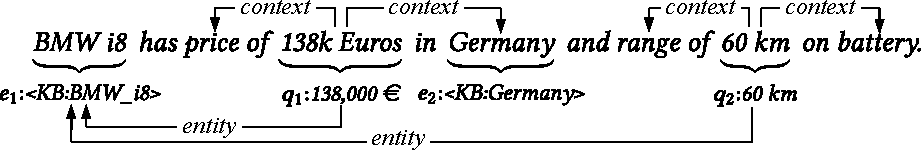
\includegraphics[width=0.5\textwidth]{figures/example_2}
\vspace{-2em}
\end{figure}

With the above example, we can extract two Qfacts: $\mathcal{F}_1 = (e = \textit{<KB:BMW\_i8>}; q = \textit{(138.000; \euro)}; X = \{\textit{price}, \textit{Germany}\})$ and $\mathcal{F}_2 = (e = \textit{<KB:BMW\_i8>}; q=\textit{(60; km)}; X = \{\textit{range}, \textit{battery}\})$.
We extract seed Qfacts from three large collections of text documents - the STICS project \cite{DBLP:conf/sigir/HoffartMW14}, the New York Times archive \cite{nyt}, and English Wikipedia, 
% \footnote{\url{https://meta.wikimedia.org/wiki/Data_dump_torrents\#English_Wikipedia}}
 containing a total of 13.4M documents. Extracted Qfacts from text are filtered by confidence, duplicate-removed, organized and indexed to serve the column alignment task 
 on web tables later.


\end{comment}
%!TEX root = ../main.tex
%\section{Quantity Search on Web Tables}
\section{Use Case: Quantity Querying}
\label{sec:querying}
\subsection{Matching and Ranking}

%%%GW: keep this short, as it is essentially the same as in the ISWC 2019 paper

\begin{comment}


In this section, we describe our quantity search system on web tables, built on top of the extraction model described in Sections \ref{sec:extract} and \ref{sec:qfact_scoring_model}. Figure \ref{fig:search_ov} shows the overview of our system, which contains two main phases: \textit{Extraction} and \textit{Search \& Ranking}.

\end{comment}

All Qfacts from web tables are fully contextualized into the form
$\mathcal{F} = (e,q,X)$, stored and indexed.
% , along with their
% combined evidence scores, in ElasticSearch.
We process a Qquery $\mathcal{Q} = (qt,qq,qX)$
against this data
by mostly following the method of \cite{DBLP:conf/semweb/HoIPBW19}:
Qfact entities are matched against the target type $qt$ using type information from the KB, quantities are compared to query condition $qq$,
and the context agreement between $X$ and
$qX$ is quantified by the
{\em directed embedding distance} of \cite{DBLP:conf/semweb/HoIPBW19}.
This yields a ranking of entity answers to a given query.

We extend the context comparison, as our setting
differs from \cite{DBLP:conf/semweb/HoIPBW19}.
In text-based Qfacts, the context tokens come
from the same sentence or short snippet.
In contrast, for the table-based setting, we combine 
a set of cues from different kinds of context: Q-column header, page title, table caption, DOM-tree headings, same-row cells, and surrounding text window. 
%\m{This work considers the immediate paragraph preceding and following the table as the text window.}
%%%GW: I clarified this in Section 3.4 on Contextualization, no need to have it here again
To reflect this heterogeneity, we assign tunable weights
to the context tokens based on their origin. 

\vspace{0.1cm}
\noindent {\bf Definition [Weighted Directed Embedding Distance].}
% \vspace{0.1cm}
$$\textit{w-ded}(X,qX) = \Bigg( \sum\limits_{u \in qX} 
\omega(u) \cdot \min\limits_{v \in X}
(\sigma(v) \cdot d(u,v))
\Bigg)
~/~
\Bigg( \sum\limits_{u \in qX} \omega(u) \Bigg)$$
% \vspace{0.1cm}
with $\omega$ denoting tf-idf-based weights of tokens
and $\sigma(v)$ denoting the weight of Qfact context
token $v$ depending on the kind of context from where
it originates. We have six different $\sigma$
weights for the six kinds of context considered (see above); they are not word-specific.
$d(u,v)$ is the word2vec embedding distance between
two words $u$ (from the query) and $v$ (from the answer candidate). In essence, this directed scoring function finds for each Qquery context word $u$ the best matching token $v$ from the Qfact context, taking context type into account by using $\sigma(v)$.
% Note that this directed scoring penalizes situations when the Qfact context has many additional tokens that are not present in the query context, to mitigate topical drifts \cite{DBLP:conf/semweb/HoIPBW19}.


%%%GW: polished/rewrote this paragraph
\begin{comment}

Context agreement \textit{w-ded} is then combined with quantity similarity and entity prominence to produce Qfact relevance score:
\[
\textit{rel-score}(\mathcal{F}) = \alpha \cdot \textit{w-ded}(X,qX) + \beta \cdot \textit{sim}(q,qq)
+ \gamma \cdot \textit{prom}(e)
\]
where $\textit{sim}(q,qq)$ is measured using relative numeric distance, entity prominence $\textit{prom}(e)$ is computed from Wikipedia page-view, and $\alpha$, $\beta$, $\gamma$ are hyper-parameters. Prior work \cite{DBLP:conf/semweb/HoIPBW19} treats quantity condition $qq$ merely as a filter. We extend this by additionally taking quantity similarity into account, which boosts Qfacts, whose quantity $q$ has the same order of magnitude as the query quantity $qq$. 
For example, when searching for stadiums with a capacity above 50,000, we expect
all answers to be somewhere between 50,000 and say 200,000, but values in the millions would be suspicious (e.g., when confusing the annual ticket sales with capacity).
Optionally, we consider also entity prominence to ensures that important entities are prioritized to show to the user.
\end{comment}

%%%GW: commented out

\begin{comment}

In addition to the context-agreement score {\em w-ded}, we consider another
signal for a Qfact matching the query, by comparing the Qfact quantity $q$ against
the query quantity $qq$. Prior work \cite{DBLP:conf/semweb/HoIPBW19} treats quantity condition $qq$ merely as a filter. We extend this 
by computing a penalty score
% for $q$ and $qq$: 
$\textit{pty}(q,qq) \propto  e^{\frac{|q-qq|}{\max(|q|,|qq|)}} - 1$ 
that penalizes $q$ values that are \textit{excessively} larger or smaller than $qq$.
% , with parameter $\varepsilon$ controls the sensitivity of the penalty.
% For queries with conditions other than ``above $qq$'', the score is compute analogously.
% by additionally taking quantity similarity $\textit{sim}(q,qq)$ into account, using relative numeric distance.
The intuition here is that $q$ should of the same order of magnitude as $qq$.
For example, when searching for stadiums with a capacity above 50,000, we expect
all answers to be somewhere between 50,000 and say 200,000, but values in the millions would be suspicious (e.g., when confusing the annual ticket sales with capacity).

Finally, for the overall ranking of query results, we optionally consider also the entity prominence
% of the returned entity 
$\textit{prom(e)}$, computed from Wikipedia page-view statistics, to ensure that important entities are prioritized to show to the user.


The overall relevance score of a Qfact for a given Qquery is then set to:
\[
\textit{rel-score}(\mathcal{F}) = \alpha \cdot \textit{w-ded}(X,qX) - \beta \cdot \textit{pty}(q,qq)
+ \gamma \cdot \textit{prom}(e)
\]
with hyper-parameters $\alpha, \beta, \gamma$.
\end{comment}
% \GW{I rewrote this paragraph. Please read carefully. Note that I wanted the penalty effect for q exceeding qq to be very small initially and be influential only when q goes into a different order of magnitude, hence the suggestion for the exponential function!!!} 

% \todo{this exponential function is wrong, it only takes into account the difference of q-qq, not the magnitude: example: 5-10 is different from 50-55, relative numeric distance is better, I rewrote}


\begin{comment}

\subsection{Extraction} In this phase, we offline process all input tables to extract Qfacts and save them into a storage. For each web table (Block 1), we preprocess to recognize quantities and detect candidates for each entity mention. Afterwards, our described joint model is applied to disambiguate named entities and find the alignment between quantity and entity columns, with the support of a collection of external text documents (Block 2).

Then, Qfacts $\mathcal{F} = (e,q,X)$ from processed tables are extracted 
% based on the detected entity annotations and column alignment
. In particular, 
%given processed table $\mathcal{T} = (r, c, \mathcal{H},\mathcal{B}, \mathcal{X})$,
 we extract a Qfact for each row $i$ and column link $\mathcal{C}_{k} 
\rightarrow
\mathcal{C}_{v}$, with entity $e \in b_{i,v}$, quantity $q \in b_{i,k}$, and context $X = h_k \cup \{b_{i,?} | ? \neq k, v\} \cup \mathcal{X}$. Here, we include not only the header $h_k$ of the quantity column into $X$, but also other related components of the table: \textit{(1)} cells $b_{i,?}$ in the same row $i$, except $b_{i,k}$ and $b_{i,v}$; and $\mathcal{X}$ -- the table surrounding context, including: \textit{(2)} table caption; \textit{(3)} page title; \textit{(4)} page content (we only take the paragraphs close to the table); and \textit{(5)} additionally for Wikipedia tables, the section titles lying on the XPath of the table, extracted from the page DOM tree. This is because important information to query might not contained in the table alone, but in the components outside it. 

Extracted Qfacts are saved into a storage (Block 3), where entities are augmented with their type information from the KB, and quantities are linked to the QuTree unit catalog \cite{DBLP:conf/kdd/SarawagiC14} to allow comparison.

\subsection{Search \& Ranking} In this phase, we answer given quantity queries by matching them against extracted Qfacts (Block 4).
First, following \cite{DBLP:conf/semweb/HoIPBW19}, we decompose the input question into Qquery format $\mathcal{Y} = (t^*,q^*,X^*)$ by a rule-based parser. The parser uses a dictionary of YAGO types and a dictionary of quantity units to recognize the target type of answers $t^*$ and the quantity condition $q^*$. Then, all remaining tokens of the query (except stopwords) are included in the query context $X^*$.

We score each candidate Qfact $\mathcal{F} = (e,q,X)$ by perform Qquery-Qfact matching, which consists of entity-type matching, quantity matching, and context matching. Following \cite{DBLP:conf/semweb/HoIPBW19}, based on type information of $e$, we do entity-type matching by discarding $\mathcal{F}$ if $e$ is not an entity of type $t^*$. Then, we do quantity matching between $q$ and $q^*$ with the support of a list of unit conversion rules from QuTree catalog \cite{DBLP:conf/kdd/SarawagiC14}. If $\mathcal{F}$ passes these two filters, we give it a score by matching context. Since Qfact context tokens $X$ might come from various parts of the table, we propose a weighted version of the \textit{directed embedding distance} \cite{DBLP:conf/semweb/HoIPBW19} for context matching as:
\begin{align*}
\textit{w-ded}(\mathcal{F}, \mathcal{Y}) 
% &= \textit{w-ded}(X^* \rightarrow X) \\
&= \bigg(\sum\limits_{u \in X^*} W(u)\min\limits_{v \in X}\big(L(v)\ d(u,v) \big)\bigg)\big/\sum\limits_{u \in X^*}W(u) 
\end{align*}
The only difference between \textit{w-ded} and \textit{ded} is that \textit{w-ded} considers the locational weights $L(v)$ of the Qfact context tokens, which indicates the importance of where the token is (e.g., a match in table header or table caption is more important than in page content). The locational weights of table header, table caption, page/section titles, same-row cells and page content are empirically tuned 
based on 
% the results from 
a small set of ten queries.

%we fix the locational weights of table header, table caption, page/section titles, same-row cells and page content to 1.0, 0.9, 0.8, 0.8 and 0.7, respectively.

\end{comment}

%%%%%%%%%%%%%%%%%%%%%%%%%%%%%%%%%%%%%%%%%%%%%%%%%%%%%%%%%
%%%GW: new contribution, hence need to highlight by its own subsection !!!

\subsection{Corroboration by Inter-Fact Consistency}
\label{subsec:consscore}

%\vspace{0.1cm}
%\noindent \textbf{Consistency-based Qfact Corroboration}.
%
\begin{comment}
Scoring using \textit{w-ded} only looks at the candidate Qfact itself 
(i.e., Qfacts are treated independently). As the query context is relatively short comparing to Qfacts context (combined from various parts of the table), this might put some noise in the results as several tiny cues from Qfact context can totally change its meaning. A potential solution to demote these noisy Qfacts, and as a result, promote good Qfacts is to consider also the similarity between them (i.e., similar Qfacts should be scored close to each other). 
% \sr{I suppose the idea has two parts - similar facts should score similar, but also, facts that have many closely similar facts should score higher than those with few similar facts?}
We propose a consistency-based approach to re-score candidate Qfacts, as described below.
\end{comment}

We use the 
\textit{w-ded} distances
% relevance scores 
between
candidate answers and the query as 
%a prior (weakly confident score), to compute for each candidate Qfact a posterior consistency score $\textit{cst}(\mathcal{F})$, by learning information from other Qfacts in the candidate list.
%%%GW: avoid the wording prior and posterior here, as it is often used to denote Bayesian inference - which is not the case here
{\em initial scores} for answer ranking.
%%%GW: give intuition first
This initial ranking is further improved by considering
the {\em mutual consistency} among the answer facts
for the same query.
To this end, we can exploit that our data often
yields several Qfacts for the same answer entity.
If all or most of them agree on their quantities and
contextual cues, 
% this should boost their final scores
their scores should be close
to each other.
This idea can be generalized to all answer candidates
even if they differ in their entities:
they should still mostly agree on their contextual cues,
and their quantities should have comparable order
of magnitude.
For example, if the candidate pool for answering
a query about 
%``British football clubs with value
%above 1.5 billion pounds'' includes spurious
%results like 
``British football stadiums with a seating capacity above 50,000'' includes spurious results like
%({\small\tt Arsenal FC, 5,925 \pounds}, 
%$\{$football, London, season, ticket$\}$), 
%or 
%({\small\tt Real Madrid, 4,200,000,000 \euro},
%$\{$football, Spain, asset$\}$),
(\textit{Wembley Stadium, 32,000,000, 
``world cup, 1966, TV viewers''}), 
or 
(\textit{Maracana Stadium, 78,838,
``FIFA, Rio, 2014''}),
these stand out against many good results
by having the wrong order of magnitude in
quantities or by missing important contextual cues about UK.

To detect and leverage such situations for
elimination or demotion of noisy results, 
we have devised a method for
consistency-aware corroboration and re-scoring
of answer candidates.
This is inspired by earlier work on consistency learning
for image classification 
\cite{DBLP:conf/mir/YagnikI07}. 
Algorithm \ref{algor:2} 
%sketches a scheme to estimate consistency score 
%based on a discriminative approach, 
outlines this method.
%which we generalize from the earlier work \cite{DBLP:conf/mir/YagnikI07}. 
%Key insight in the method is the observation that samples that confirm to classifiers learned from an unbiased set of weak hypothesis have a higher probability of correctness. 

\begin{algorithm}[t]
%  \small
\DontPrintSemicolon
\SetKwInOut{Input}{Input}
\SetKwInOut{Output}{Output}
\SetKwProg{Fn}{Function}{}{}
\SetKwRepeat{Do}{do}{while}
\Input{\ Candidate Qfacts $\mathbb{F} = \{\mathcal{F}_1, \mathcal{F}_2, ... | \mathcal{F}_i = (e_i,q_i,X_i)\}$\\
%along with their prior scores for the given Qquery}
with initial scores for Qquery $\mathcal{Q} = (qt,qq,qX)$}

%\Output{\ Posterior consistency scores of candidate Qfacts}
\Output{\ Consistency-aware scores of candidate Qfacts}

Sample randomly a probe set from the candidate list $\mathbb{P} \subset \mathbb{F}$. \\

Train a Qfact quality predictor from the remaining candidate Qfacts $\mathbb{F} \setminus \mathbb{P}$, using initial scores as ground-truth.

Run the learned predictor on the probe set $\mathbb{P}$
to compute quality scores for all Qfacts in $\mathbb{P}$.\\

Repeat steps 1-3 a large number of times.\\

The {\em consistency score} of a candidate Qfact, $\textit{cons-score}(\mathcal{F}_i)$, is computed as the average quality predicted, aggregated over all cases where $\mathcal{F}_i$ was in the probe set.\\
\caption{Consistency-based Re-scoring}
\label{algor:2}
\end{algorithm}


% The method is analogous to self-validation.
% We randomly sample a probe set from the candidate Qfacts list with
% weakly confident prior scores, and assume the remaining Qfacts
% to have true estimation to build an estimator. If the prior score
% of a Qfact in the probe set is close to its quality computed by the
% estimator, the confidence of the prior score increases. The sampling
% operation is done multiple times to ensure that the consistency
% score is not computed from a biased set of ground data.

The method is a form of self-validation,
%structurally following 
analogous to
the principle of cross-validation.
We randomly sample a probe set from the candidate Qfacts, and use the remaining Qfacts and their initial scores
as ground-truth for training a quality predictor.
The learned predictor is applied to the probe set,
and we keep track of the predicted quality scores
$\textit{cons-score}(\mathcal{F}_i)$.
%%%GW: old WSDM-submission text was good, concise and to the point, no need to fill up space
\begin{comment}
{\color{blue}
This sampling and cross-validation step is repeated
many times
to ensure that the consistency
score is not computed from a biased set of ground data.
% The final output, for each candidate $\mathcal{F}_i$ , is the average quality score
% from the predictors, aggregated over all cases
% where $\mathcal{F}_i$ was in the probe set.
}
\end{comment}

The difference between the initial score and the consistency score 
$|\textit{w-ded} - \textit{cons-score}|$ 
denotes the confidence of the initial score. A high difference between them denotes a noisy Qfact in the candidate list (i.e., either a high-ranked bad-Qfact, or low-ranked good-Qfact), which requires re-scoring. 

\vspace{0.1cm}
\noindent{\bf Definition [Re-Scoring of Qfacts].}
We re-score candidate fact $\mathcal{F}$
%=(e,q,X)$
with regard to a query
% $\mathcal{Q} = (qt,qq,qX)$
%using 
%interpolation to move the prior score towards the consistency score as follows:
as a weighted combination of initial 
score 
% \textit{rel-score}
(using $\textit{w-ded}$)
and consistency-aware $\textit{cons-score}$:
\[\textit{final-score}(\mathcal{F}) = (1 - \rho) \cdot \textit{w-ded}(\mathcal{F})~ + ~ \rho \cdot \textit{cons-score}(\mathcal{F})\]
with hyper-parameter $\rho$ to control the re-scoring effect.
%%%GW{the linear comb of initial and the diff can be rewritten as linear comb of initial and cons-score}

\vspace{0.1cm}
\noindent \textbf{Learned Predictors.} 
%As we want to handle re-scoring, even when the number of candidate Qfacts are low, we choose to use a simple k-NN method. 
As this method requires frequent re-training of
the predictor, we choose a very simple k-NN technique, which computes $\textit{cons-score}$
% based on k-nearest-neighbor.
% We represent Qfacts in a feature vector space, and  $\textit{cons-score}$ 
% is computed 
as the average initial scores
of the $k$ nearest Qfacts in the training set. 
This avoids the bottleneck of explicit re-training. 
%{\color{blue}
We define the distance between Qfacts as the weighted combination of (1) the relative numeric distance between quantities (converted to standard units) and (2) the context similarity. The latter is computed 
by a vector space model, with features comprising
% The feature vectors of Qfacts 
% comprise two signals:
the \textit{tf-idf} values of context terms weighted by the context item
from which they originate (column header, table caption, etc.).
% and the normalized quantity values
% (converted to standard units). 

%and normalized by their mean value).
% }
\begin{comment} 
\vspace{0.1cm}
\noindent \textbf{Entity Scoring}. 
Entity results are generated Qquery-Qfact matching scores. Since Qfacts are generated from different tables, many of them could share the same entity. Hence, we assign each entity a score from one of its Qfacts, which is most relevant to the Qquery. The entities are then ranked by their scores to produce the final results (Block 5).
\end{comment}
%%%GW: is this relevant for the consistency corroboration and re-scoring ???



%!TEX root = ../main.tex

\section{Evaluation}

\begin{comment}
We implemented our approach within a system prototype TabQs. A 
preliminary demo of TabQs can be found at\footnote{\textcolor{blue}{\url{http://qute-demo.webredirect.org/table/index.html}}}.
%, and conducted experiments on a Linux machine with 96 CPU cores and 1.5TB RAM. 
In this section, we demonstrate the results of our experimental evaluation, which focuses on (i) the intrinsic quality of Qfact extraction from web tables and (ii) the extrinsic quality of the end-to-end search system.
\end{comment}

%\subsubsection{Dataset.} All experiments use a large collection of news articles, compiled from two real world datasets: the \textit{STICS} project \cite{DBLP:conf/sigir/HoffartMW14} with news from 2014 to 2018, 
%and the \textit{New York Times} archive
%\cite{nyt}
% %5843811 + 1765538
%with news from 1986 to 2008.
%In total, our corpus consists of 7.6M documents.
% 
\subsection{Intrinsic Evaluation of 
%Quantity Fact Extraction from Web Tables}
QuTE Components}
\label{subsec:intrinsicevaluation}

%We conduct experiments to examine the quality of our joint model for entity linking and entity-quantity column alignment.
We present experimental results on the key components
of Qfact extraction: entity-quantity column alignment (CA) and
entity linking (EL).
The contextualization of Qfacts and
the inter-fact consistency model matter only
at query-time, and are thus evaluated in that
extrinsic use case in Section \ref{subsec:extrinsicevaluation}.

\vspace{0.1cm}
\noindent \textbf{Hyper-Parameter Tuning.}
Our method has a number of hyper-parameters
for Qfact extraction: $\lambda$ in Equation \ref{eq:joint};
%  and 
% parameters of the \textit{ext-score} when computing \textit{CA-score}, 
% and feature weights of the \textit{EL-score} (using MRF inference \todo{not sure if we need to put MRF inference here, as we do not run real full inference}, see \cite{DBLP:conf/semweb/BhagavatulaND15} for details).
% $\alpha, \beta, \gamma$ for confidence scoring; 
weights
for different context categories; and 
weights for the text-based evidence scoring model.
For tuning these, we performed a grid search to determine the configuration with the best performance on a withheld 
validation dataset.
%small validation table set.
% small validation set of ten tables.

\vspace{0.1cm}
\noindent \textbf{Testsets.}
%We evaluate  the quality of our joint approach using 
Our experiments use three table collections:
\squishlist
\item \textit{Wiki\_Links-Random:} a dataset introduced 
%from the earlier work
by \cite{DBLP:conf/semweb/BhagavatulaND15}, 
sampling 3000 tables from Wikipedia.
%originally contains 3000 tables randomly drawn from Wikipedia. 
As we are only interested in tables
that express quantity properties, 
we filter this data and obtain a set of 259 tables, referred to as \textit{Wiki\_Links-Random\_Qt}.
\item \textit{Equity:} a set of 69 
content-rich tables introduced by \cite{DBLP:conf/cikm/IbrahimRW16}. Analogously to \textit{Wiki\_Links-Random}, we 
%only pick quantitative relational tables, 
filter for tables with quantities, 
which results in a set of 30 tables, called \textit{Equity\_Qt}.
\item \textit{Wiki\_Diff}. We observe that many tables from the above two datasets are easy cases for column alignment. Very often, the linked E-column is the first one, or the table has only one E-column, so linking all Q-columns to that one is trivially correct. Hence, we compile a new dataset called \textit{Wiki\_Diff}, consisting of 134 Wikipedia tables, which are difficult cases for column alignment:
there are at least two E-columns and the referred E-column is not the first one,
%the referred entity column is not the first one,
or different Q-columns refer to different E-columns.
\squishend
All three datasets originally contain only ground truth for entity linking; we annotated them with the proper column alignment.
% , i.e, which quantity column refers to which entity column.

\vspace{0.1cm}
%\noindent \textbf{Performance of the Extraction model.}
\noindent \textbf{Performance Metrics.}
For the CA task, we 
%evaluate using the precision of correct links,
use the precision of correct alignments,
{macro-averaged} over 
tables.
%all Q-columns of all tables. 
%%%GW: averaging over all Q-columns, right???
%%%GW: alternative would be to assess complete tables, consider them as correct if all column pairs are correct, and then indeed macro-average over the tables
%
Since there are many tables where all Q-columns
refer to the same E-column, 
%using 
macro-averaging is meaningful to give each table the same weight (regardless of its width).
For entity linking (EL) the metric is the
precision, micro-averaged over entity mentions.
%over tables, so that all mentions share the same weight.
%%%GW: micro-averaged over tables doesn't make sense: averaging over tables would be macro-averaging !!!???


%\todo{move results for EL to after CA}


\begin{table}[t]

% \end{table}
% \begin{table}[t]
% \small
	\centering
		\caption{Column alignment precision \textit{(macro\_avg)}.}
	\label{tab:prec_cl}
	\vspace{\tsq}
		\begin{tabular}{l|ccc}
			    \hline
	    Method &\textit{Wiki\_L-R\_Qt} & \textit{Equity\_Qt} & \textit{Wiki\_Diff}\\ 
			    \hline
		 Leftmost & 0.736 & 0.817 & 0.045\\
 		 Most-Unique & 0.868 & 0.873 & 0.409\\
 		 Closest-Left & 0.728 & 0.674 & 0.705 \\
 		 Classifier \cite{DBLP:journals/pvldb/VenetisHMPSWMW11} & 0.864  & 0.717 & 0.597 \\
		 Iterative CA & 0.934 & 0.900 & 0.769\\ 
			    \hline
		\end{tabular}
% 	\vspace{-1em}
% 	\vspace{1.5em}
	
\end{table}
\begin{table}[t]
%  \small
% \vspace*{0.2cm}
	\centering
		\caption{Entity linking precision \textit{(micro\_avg)}.}
	\label{tab:prec_ed}
	\vspace{\tsq}
		\begin{tabular}{l|ccc} 
			    \hline
	    Method &\textit{Wiki\_L-R\_Qt} & \textit{Equity\_Qt} & \textit{Wiki\_Diff}\\
			    \hline
		  Prior & 0.849 & 0.821 & 0.846\\
		 EL-MRF \cite{DBLP:conf/semweb/BhagavatulaND15} & 0.893 & 0.863 & 0.902\\
		 Joint EL\&CA & 0.900& 0.876 & 0.902\\
			    \hline
		\end{tabular}
%	\vspace{1.5em}
\end{table}


\vspace{0.1cm}
\noindent{\bf Results for Column Alignment.}
%\subsubsection*{Column Alignment} 
We compare our \textit{Iterative CA} method with text-based evidence
against several baselines (see Section \ref{subsec:CA-priorworks}): 
\textit{(1) Leftmost}, 
%which always links quantity columns to the first column of the table, or the second column if the first one is a quantity column (i.e., index column); and 
\textit{(2) Most-Unique}, 
%which always links quantity columns to the column with the most number of unique values (also ignoring index column), prioritizing the left most one in case of a tie.
\textit{(3) Closest-Left},
and a 
\textit{(4) Classifier} with features from column-wise
properties (column-pair distances, distinct values per column, etc.) as employed by \cite{DBLP:journals/pvldb/VenetisHMPSWMW11}.

The results are shown in Table \ref{tab:prec_cl}. 
We observe that 
our \textit{Iterative CA} method outperforms all
baselines by a large margin over all three datasets.
%GW: add a strong ``strategic'' sentence:
This gives our approach a decisive advantage in
extracting more and better quantity facts from web tables.
%our column alignment approach outperforms the two baselines, especially by a large margin on \textit{Wiki\_diff} dataset.
%\todo{Show some evidence sentences from text for column linking}
\vspace{0.1cm}


\noindent{\bf Results for Entity Linking.}
%\subsubsection*{Entity Linking} 
Although our EL method mostly follows prior works \cite{DBLP:conf/semweb/BhagavatulaND15, DBLP:conf/cikm/IbrahimRW16}, we report the
performance of EL when computing jointly with CA,
%We compare our method, referred to as \textit{Joint EL\&CA}, 
against two baselines: 
\textit{(1) Prior} uses 
%a-priori frequency distributions
popularity 
of mention-entity pairs to link each mention to the
most salient entity that matches the name, and
\textit{(2) EL-MRF} \cite{DBLP:conf/semweb/BhagavatulaND15}
is a state-of-the-art method based on MRF
that incorporates priors, context similarity, row-wise coherence and column-wise coherence, but does not consider CA.
%which disambiguates using homogeneity score only, without considering entity-quantity column alignment, taking into account additional quantitative clues from text. 
%The \textit{MRF-only} baseline is actually used 
%This baseline was employed 
%by prior works \cite{DBLP:conf/semweb/BhagavatulaND15, DBLP:conf/cikm/IbrahimRW16}
%(with slightly different feature sets).
%Our novel method is referred to as \textit{Joint EL\&CA}.
%however with different sets of features. 

%Table \ref{tab:prec_ed} shows the results of this comparison.
%compares the performance between our approach and the two baselines on the three datasets. 
% joint model outperforms \textit{Prior} baseline, and works slightly better than \textit{EL-MRF} baseline. This small jump can be explained that additional quantitative clues coming from column alignment mostly affect the referred entity columns. Improvement on these referred columns could be also propagated to other entity columns through the MRF, however not significantly.
%On all three datasets, our \textit{Joint EL\&CA}
%method is as good as or better than the other methods.
Table \ref{tab:prec_ed} shows that the \textit{Joint EL\&CA}
method is 
 as good as and sometimes better than the baselines,
% on par with and sometimes better than the baselines,
on all three datasets.
%It achieves very high gains over the \textit{Prior},
%despite the fact that the tables contain many prominent entities where Prior could be expected to work well.
%It achieves very high gains over the \textit{Prior},
%despite the fact that the tables contain many prominent entities where Prior could be expected to work well.
Although the improvement over \textit{EL-MRF} is not that large, it is notable and shows the positive impact of integrating CA information on the inference of EL.
% statistically significant.
% \todo{t-test if possible, tried, but don't have time enough time for this, make this softer!!!!!}

%%%%%%%%%%%%%%%%%%%%%%%%%%%%%%%%%%%%%%%%%%%%%
%{\color{blue}
\vspace{0.1cm}
\noindent{\bf Ablation Study.} To analyze the influence of different components of %method for column alignment, 
our CA method,
we conducted a comprehensive ablation study, by selectively disabling the following components:
(1) type-based evidence for text-based scoring, and
(2) coreference resolution for entity mentions when building the background Qfact collection from text.
The results are shown in Table~\ref{tab:ablation_CA}.  

We observe that without type-lifted evidences, the CA precision decreases by more than 10 percent on all three datasets; for the difficult dataset \textit{Wiki\_Diff}, performance even drops by 50 percent. 
Exact-entity matching alone is 
%inefficient as it requires the same information about a table-Qfact to be present also in text, which is often not the case.
insufficient as it suffers from the sparseness.
This emphasizes the decisive role of our novel contribution to
leverage external text evidence, as opposed to prior works that restricted information extraction from web tables to the tables themselves (and their local context).
%
Disabling coreference resolution, for collecting background Qfacts from text, also degrades precision, but to much lesser degree: 5 percent at most.
%also shows visible improvement for calculating evidence score. The reason is that many useful Qfacts cannot be extracted directly from individual sentences, where the entity appears in the form of nominal or pronominal mentions, which requires coreference resolution.

% Coreference resolution can tackle this problem and expand the diversity of the background Qfact collection.

% I wanted to emphasize 'diversity', because many 'kind of' information cannot be found from individual sentence, like ... I don't know, something is never mentioned along with entity in a single sentence.

%}
%%%%%%%%%%%%%%%%%%%%%%%%%%%%%%%%%%%%%%%%%%%%%%%%%



\begin{table}[t]
%{\color{blue}
    % \small
	\centering
		\caption{Ablation study results for CA.}
	\label{tab:ablation_CA}
	\vspace{\tsq}
		\begin{tabular}{l|ccc}
			    \hline
	    Method &\textit{Wiki\_L-R\_Qt} & \textit{Equity\_Qt} & \textit{Wiki\_Diff}\\ 
			    \hline
			    Iterative CA & 0.934 & 0.900 & 0.769\\ 
			    \hline
		 {\hspace{0.25em}$-$ type-based evidence} & 0.796 & 0.617 & 0.254 \\
 		 {\hspace{0.25em}$-$ coreferences} & 0.877  & 0.892 & 0.728 \\
			    \hline
		\end{tabular}
% 	\vspace{-1em}
%}
\end{table}



\subsection{Extrinsic Evaluation of 
%the End-to-End Search System}
%Use Case: 
Search and Ranking}
\label{subsec:extrinsicevaluation}
%We evaluate our end-to-end TabQs system for large scale search on a large collection of web tables.
This section presents experimental results for an end-to-end use case of
quantity queries and their result rankings.

\vspace{0.1cm}
\noindent \textbf{Hyper-Parameter Tuning.}
Analogously to 
%the intrinsic evaluation of
Section \ref{subsec:intrinsicevaluation},
we tune query-time hyper-parameters for the
% relevance \textit{rel-score} 
\textit{w-ded} distance
and for the mixture with
\textit{cons-score} (see Section \ref{subsec:consscore})
by grid search for 
best Precision@10 on a withheld validation set.
%of ten queries.
% and their answers.

\vspace{0.1cm}
\noindent \textbf{Dataset.}
We run queries on a large collection of web tables
compiled from two major sources:
%\begin{enumerate}[leftmargin=*]
\squishlist
\item \textit{TableL} was introduced by \cite{DBLP:conf/icde/IbrahimRWZ19}.
It contains 2.6M tables from 1.5M web pages, mostly falling under five major topics: finance, environment, health, politics, and sports.
\item \textit{Wikipedia Tables}, first introduced by \cite{DBLP:conf/semweb/BhagavatulaND15}. 
%Unfortunately, this corpus is quite old, and only contains the tables alone, without including the web pages' content. Hence, 
As the original collection from 2015 is outdated,
we processed a recent version of the English Wikipedia XML dump (March 2020) 
% using the Sweble parser \cite{DBLP:conf/wikis/DohrnR11}, 
to construct an analogous dataset, containing a total of 1.8M tables.
% In particular, we extracted all HTML tables from Wikipedia which have the class attribute ``wikitable'', %
% resulting in a dataset of 1.8M tables.
%
% WD fact 88680715 entity 12741586
%\end{enumerate}
\squishend
%Not all of these tables are relevant for our purpose (relational \& quantitative). Table \ref{tab:stats} shows statistics of the large scale extraction, where we report the number of quantitative relational tables, the number of extracted Qfacts, and the number of extracted entities for each table corpus. In total, we end up with 618K tables and 18.8M extracted Qfacts, ready for large scale search.
The combined collection was filtered for tables that
contain both E-columns and Q-columns.
Table \ref{tab:stats} shows data statistics
of the large scale extraction, where we report the number of filtered E-Q-tables, the number of extracted Qfacts, and the number of extracted entities for each table corpus.
In total, we end up with 618K tables and 18.8M extracted Qfacts, ready for large scale search.

%\todo{Wikidata: 555 numeric predicates, MOVE to motivation instead} \sr{555 is quite much - perhaps few have data (e.g., more than 100 statements? Or maybe best to drop this argument}

\begin{table}[t]
%  \small
	\centering
		\caption{Table collection statistics.}
	\label{tab:stats}
	\vspace{\tsq}
% 		\setlength{\tabcolsep}{0.34em}
		\begin{tabular}{l|rrrr} 
			    \hline
	    Source & \textit{\#tables} & \textit{\#E-Q-tables} & \textit{\#distinct-entities} & \textit{\#qfacts}\\
			    \hline
            % th0.6
            % 8865788 / 339395 / 756892
		  Wikipedia & 1.8M & 339K  & 757K  & 8.87M \\
		  % 9943672 / 278111 /255182
		 TableL & 2.6M & 278K  & 255K & 9.94M \\
		 \hline
		  % 18809460 / 617506 / 863248
		 Total & 4.4M & 618K  & 863K & 18.81M \\
			    \hline
		\end{tabular}
\end{table}


\vspace{0.1cm}
\noindent \textbf{Query Benchmarks.}
We use two sets of telegraphic queries:
\squishlist
\item \textit{Q100:} an established benchmark of 100 quantity queries from \cite{DBLP:conf/semweb/HoIPBW19}, 
featuring questions on a range of quantity measures for four domains: \textit{Finance}, \textit{Transport},
\textit{Sports} and \textit{Technology}.
Ground-truth answers are annotated as \textit{relevant} or \textit{irrelevant}
for the top-10 results of the original, text-based work in \cite{DBLP:conf/semweb/HoIPBW19}.
We extend these annotations to the top-10 results of all
methods under comparison.
However, there is no ground-truth about ideal top-10 results,
like lists of {\em all} answers or answers sorted in ascending or descending order
of quantity value (e.g., the largest stadiums for a query about ``sports arenas with
capacity above 50K''). So there is no way to evaluate recall with this benchmark.
\item \textit{NewQ150:} To allow evaluating both precision and recall,
we constructed a new collection of 150 queries, similar in nature to those of Q100
but such that each of them has a ground-truth answer list.
To this end, we identified Wikipedia list pages that either capture the
desired query result or provide a superset that is sorted by the quantity of interest. Examples for this kind of ground-truth is a list of all sprinters
who ran 100 meters under 10 seconds, which by its sorting, also provides a sub-list
of results under 9.9 seconds.
%Examples for this kind of ground-truth are
% a Wikipedia list of the largest football stadiums, or 
% a list of all sprinters
% who ran 100 meters under 10 seconds, which by its sorting, also provides a sub-list
% of results under 9.9 seconds.
%our self-compiled 200 questions with a limited number of relevant answers (e.g., building higher than 500 m), which is used for measuring recall. \todo{confirm 200 questions} We call these two question sets \textit{Query-100} and \textit{Q-recall-200}, respectively. The ground truth target answers for questions in \textit{Q-recall-200} are manually collected in advance. Table \ref{table:example_qa} presents some anecdotal example quantity queries and their answers produced by TabQs.
\squishend

%For each query, top-10 entity answers are manually annotated as \textit{relevant} or \textit{irrelevant} based on the cue given in the corresponding tables from which they are extracted. In the case of Google baseline, as produced answers are snippets, these snippets are annotated as relevant if they mention an entity and a quantity that the query. 

\vspace{0.1cm}
\noindent{\bf Performance Metrics.}
For both benchmarks, we report  \textit{Precision@10}, 
%and \textit{Hit@3}
% and \textit{Mean-Reciprocal-Rank (MRR)}
macro-averaged over 100 or 150 queries, respectively. 
%Moreover, for \textit{Q-recall-200}, as target answers are known, 
%% the evaluation can be done automatically, 
For NewQ150, we also report \textit{Recall@10} and \textit{mAP@10} with
regard to the 
% top-10
answers in the ground-truth list.
% , and when possible also complete \textit{MAP} with regard to the entire ground-truth list of expected answers.

%we also report \textit{Mean-Average-Precision (mAP)}, \textit{Recall@10} and \textit{Recall} (from top \textit{k} answers, where \textit{k} is the groundtruth size, varies for different queries). We do not do this for \textit{Query-100}, as it requires exhaustively annotating a huge pool of candidate answers. %Table \ref{table:performance_tabqs} compares the performance between TabQs and the two baselines.
% for both question sets. 
%\todo{comment, show a screenshot of search system?}
%GW: no screenshot

\vspace{0.1cm}
\noindent \textbf{Baselines.} 
% \todo{I think we need to emphasize that we are the only quantity search engine working on tables, otherwise reviewers will say that baselines are not comparable, need something else,... but they can't point out what are the 'else'????}
%{\color{blue}
To the best of our
knowledge, QuTE is the first system addressing quantity filters based on web tables. Therefore, there is no direct reference baseline; instead we compare against two strong baselines
on quantity search over textual and general web contents:
%}
% We compare QuTE against two strong baselines:
\squishlist
\item \textit{Qsearch} is a text-based quantity search engine \cite{DBLP:conf/semweb/HoIPBW19,DBLP:conf/wsdm/HoPKBW20}
(accessible at \textit{\url{https://qsearch.mpi-inf.mpg.de/}}).
It runs on a collection of 21.7M Qfacts automatically extracted from
sentences in Wikipedia articles and 
%two large news corpora,
%the New York Times archive and the STICS corpus
%\cite{DBLP:conf/sigir/HoffartMW14}.
news articles from the New York Times archive and web crawls.

This setup is not comparable to our QuTE method, as the underlying data sources
are  not the same. Nevertheless, having this baseline gives insights on the value of tapping 
into web tables.
%we compare TabQs with the Qsearch \cite{DBLP:conf/semweb/HoIPBW19} system. To the best of our knowledge, this is the only system that can handle quantity queries and produce crisp entity answers as we do. However, while Qsearch searches for answers from text, our TabQs system looks into web tables. \sr{Say here on which texts Qsearch operates, and argue why the comparison is fair (e.g., Wikipedia text vs.\ Wikipedia tables, or a huge text web crawl versus a huge table web crawl} 
%
\item \textit{Google} serves as the reference point for search-engine methodology.
When we pose our benchmark queries, Google returns ten blue links along with preview snippets.
The results are typically a mix of highly informative snippets, irrelevant snippets,
and links to authoritative lists. These list pages often contain very good results,
but the user would have to explicitly access and browse them (as opposed to being
provided with direct answers in terms of entities).
\squishend
%
For Google results, 
we assess the top-10 answer quality (with regard to the ground-truth top-10)
in two different modes: 
\squishlist
\item \textit{Direct answers (Google-DA):} 
%[Google-S]:} 
%%%GW: this sounds like a variant of the system/baseline itself, but it is merely a different mode of evaluating
only named entities that appear in the preview snippets are 
considered. This is a conservative mode, assuming lazy users who do not engage on
further browsing.
\item \textit{List expansion (Google-LE):}
%[Google-L]:} 
each list-page answer (with the word ``list'' in its title)
is fetched to materialize the list of entities, in the order of the list itself.
Conceptually, this is done for each top-10 result of this kind, and the resulting lists
are concatenated. 
% The ground-truth list (from Wikipedia) is discounted.
The top-10 entities are considered as query answers in this mode, where users continue browsing.
\squishend
%Second, even through TabQs produces entities as main result, we still want to compare it with a standard search system, which produce snippets. 
%In particular, we run all benchmark queries on Google web search and retrieve top-10 snippets for each of them.


%%%%%%%%%%%%%%%%%%%%%%%%%%%%%%%%%%%%%%%%%%%%%%%%%%%%%%%%%%%%%%%%%%%%%%%%%%%%%%%%%%%%%%%%%%%%%%%


%% \begin{table*}[t]
% \caption{End-to-end evaluation of TabQs. \sr{Consider also showing for one line, mocks of the actual Wikipedia tables from which the first 4 results are extracted (in super small)? This would increase plasticity of the presentation - as so far the paper contains no real Wikipedia table screenshot}}
% \vspace{-0.5em}
% \setlength{\tabcolsep}{0.34em}
% \centering
% \begin{tabular}{l|ccc|ccc|ccc|ccc|ccc}
%           \midrule
%  \multirow{2}{*}{\textbf{Metric}} & \multicolumn{3}{c}{\textbf{Finance}} & \multicolumn{3}{|c}{\textbf{Transport}} & \multicolumn{3}{|c}{\textbf{Sports}} & \multicolumn{3}{|c}{\textbf{Technology}} & \multicolumn{3}{|c}{\textbf{ All}} \\
%  \cmidrule{2-16}
%   &  \textit{Google} & \textit{Qsearch} &  \textit{TabQs} &
%   \textit{Google} & \textit{Qsearch} &  \textit{TabQs}&
%     \textit{Google} & \textit{Qsearch} &  \textit{TabQs}&
%       \textit{Google} & \textit{Qsearch} &  \textit{TabQs}&
%   \textit{Google} & \textit{Qsearch} &  \textit{TabQs}   \\
%           \midrule
% \textbf{Pr.@1} & & & & & & & & & & & & & & &\\
% \textbf{Pr.@3} & & & & & & & & & & & & & & &\\
% \textbf{Pr.@5} & & & & & & & & & & & & & & &\\
% \textbf{Pr.@10} & & & & & & & & & & & & & & &\\
% \midrule
% \textbf{Hit@3} & & & & & & & & & & & & & & &\\
% \textbf{Hit@5} & & & & & & & & & & & & & & &\\
% \midrule
% \textbf{MRR} & & & & & & & & & & & & & & &\\
%           \midrule
% \end{tabular}
% \label{table:performance_tabqs}
% \end{table*}

\begin{table}[t]
  \small
  \caption{End-to-end evaluation of TabQs. \note{GG: normal mode}}
  \note{list mode for Google-q-recall: report separately in text\\
Pr.1: 0.407\\
Pr.3: 0.458\\
Pr.5: 0.476\\
Pr.10: 0.442\\
  Rec@10: 0.315}
  \vspace{-1em}
  \setlength{\tabcolsep}{0.25em}
  \centering
  \begin{tabular}{l|cccc|cccc}
    \hline
    \multirow{2}{*}{\textbf{Metric}} & \multicolumn{4}{c}{\textit{\textbf{Query-100}}} & \multicolumn{4}{|c}{\textit{\textbf{Q-recall-177}}}\\
    \cline{2-9}
    &  \textit{Google} & \textit{Qsearch} &  \textit{QuTE} & \textit{QuTE-rs} &
    \textit{Google} & \textit{Qsearch} &  \textit{QuTE} & \textit{QuTE-rs}\\
    \hline
    \textbf{Pr.@1}   &  0.340  & 0.690 & 0.490 & 0.510 &  0.209  & 0.390 & 0.528 & 0.525 \\
    \textbf{Pr.@3}   &  0.310  & 0.617 & 0.493 & 0.528 &  0.198 & 0.367 & 0.487 & 0.492 \\
    \textbf{Pr.@5}   &  0.280  & 0.559 & 0.484 & 0.519 & 0.193  & 0.328 & 0.456 & 0.465 \\
    \textbf{Pr.@10}  &  0.274  & 0.492 & 0.453 & 0.486 & 0.169  & 0.285 & 0.416 & 0.429 \\
    \hline
    \textbf{Hit@3}   &  0.570  & 0.840 & 0.590 & 0.617 & 0.418  & 0.644 & 0.706 & 0.723 \\
    \hline
    \textbf{Rec.@10} & -- & --    & --    & --    &  0.078  & 0.175 & 0.276 & 0.282 \\
    \textbf{Recall}  & -- & --    & --    & --    & -- & 0.229 & 0.369 & 0.378 \\
    \hline
    \textbf{mAP}     & -- & --    & --    & --    & -- & 0.185 & 0.339 & 0.342 \\
    \hline
    \textbf{Diff@10}     & -- &  4.180  & --    & 3.830   & -- & 1.254 & -- & 2.684 \\
    % \textbf{Comm@10}     & -- & --    & --    &  0.570   & -- & --& -- & 1.508 \\
    
    \hline
  \end{tabular}
  \label{table:performance_tabqs}
\end{table}

%\vspace{0.1cm}
\begin{table}[t]
%   \small
  \caption{Performance results for \textit{Q100}.}
	\vspace{\tsq}
  \centering
  \begin{tabular}{l|ccc} \hline
 System & \textit{Prec.@1} & \textit{Prec.@5} & \textit{Prec.@10} \\ \hline
 Google-DA & 0.340 & 0.280 & 0.274 \\ 
%  \hline
 Google-LE & 0.460 & 0.518 & 0.462 \\ 
%  \hline
 Qsearch & 0.690 & 0.559 & 0.492 \\ 
%  \hline
 QuTE & 0.540 & 0.512 & 0.491  \\ \hline
 \end{tabular}
  \label{table:performance_Q100}
  
%   \vspace{1.5em}
  \end{table}
\begin{table}[t]

    % \small
  \caption{Performance results for \textit{NewQ150}.}
	\vspace{\tsq}
%   \setlength{\tabcolsep}{0.25em}
  \centering
  \begin{tabular}{l|ccc} \hline
System & \textit{Prec.@10} & \textit{Recall@10} & \textit{mAP@10} \\  \hline
    {Google-DA} & 0.167 & 0.076 & 0.041  \\ 
    % \hline
    {Google-LE} & 0.342 & 0.251 & 0.193 \\ 
    % \hline
    {Qsearch} & 0.290 & 0.177  & 0.119  \\ 
    % \hline
    {QuTE} & 0.519 & 0.341  & 0.294  \\  
    \hline
  \end{tabular}
  \label{table:performance_newQ150}
\end{table}

%!TEX root = ../main.tex
\begin{table*}[t]
	\caption{Anecdotal examples of quantity queries and top results by QuTE.}	
	\small	
	\vspace{\tsq}
	\begin{tabular}{l|l} 	 
				    \hline
		Query & Top Results \\    \hline
		Skyscrapers higher than 1000 feet & Empire State Building, One World Trade Center, The Shard, Chrysler Building, etc. \\ 
    British football teams worth more than 1.5 billion pounds & Manchester United F.C., Arsenal F.C., Liverpool F.C., Chelsea F.C., Manchester City F.C.\\  
		 Sprinters who ran 100 meters under 9.9s & Usain Bolt, Carl Lewis, Maurice Greene,  Justin Gatlin,	Christian Coleman, etc.  \\  

		Mobile games with number of players more than 250 million & Angry Birds, Super Mario Run, Candy Crush Saga, Temple Run, Pok\'{e}mon Go, etc. \\ 

			    \hline
	\end{tabular}	
	\label{table:example_qa}
\end{table*}
%\noindent \textbf{Performance of TabQs.}

\vspace{0.1cm}

\noindent{\bf Main Results.}
The precision results for the \textit{Q100} benchmark are shown in
Table \ref{table:performance_Q100}.
We see that Qsearch performs best for the top rank alone,
but drops in precision with more results.
This is because it is designed to retrieve a few
high-confidence results and has very limited
recall due its data based on single sentences.
QuTE has lower precision but keeps this fairly
high also for lower ranks, being able to find
more correct answers from its table collection.
The weak results for Google-DA show that
search engines are really missing the ability
to compute direct answers for quantity filters.
Google-LE performs better, benefitting from
list expansion because it often has one or two
good super-lists of proper results in its 10 
``blue links''.
%

The results for the \textit{NewQ150} benchmark are shown in
Table \ref{table:performance_newQ150},
including recall and mAP for the top-10 query results.
Here we see that QuTE clearly outperforms all
baselines, especially in terms of recall@10 and
mAP@10. Extracting Qfacts from web tables with high yield
enables QuTE to compute many correct answers. 
Qsearch is limited by its text-based pool of candidate answers.
The search engine again shows its missing support
for quantity filters in direct-answers mode;
in list-expansion mode, it performs much better
but is still inferior to QuTE.
%

Table \ref{table:example_qa} shows a few anecdotal query results obtained by QuTE.
%

% \begin{table}[t]
%   \small
%   \caption{Performance study of QuTE vs. QuTE-rs.}
%   \vspace{-1em}
%   \setlength{\tabcolsep}{0.25em}
%   \centering
%   \begin{tabular}{c|c|cccc|c|c}
%     \hline
%     \multirow{2}{*}{\textbf{Benchmarks}} & \multirow{2}{*}{\textbf{Methods}} & \multicolumn{4}{c}{\textit{\textbf{Metric}}} \\ 
%     \cline{3-8}
%     & & \textit{Pr.@1} & \textit{Pr.@3} &  \textit{Pr.@5} &  \textit{Pr.@10} & \textit{Recall} & \textit{mAP} \\ \hline
%   \multirow{2}{*}{\textbf{\textit{Q100}}} & \textbf{QuTE}    &  0.510 & 0.528 & 0.519 & 0.486 & -- & -- \\
%     &\textbf{QuTE-rs} & 0.490 & 0.493 &  0.484 & 0.453 & -- & -- \\ \hline
%     \multirow{2}{*}{\textbf{\textit{NewQ150}}} & \textbf{QuTE}    &  0.533 & 0.509 & 0.482 & 0.446  & 0.380 & 0.356 \\
%     &\textbf{QuTE-rs} & 0.540 & 0.504 &  0.473 & 0.432 & 0.380 & 0.352 \\
%     \hline
%   \end{tabular}
%   \label{table:ablation_study}
% \end{table}

\begin{table}[t]
%{\color{blue}

%   \small
  \caption{Ablation study results on \textit{Q100}.}
	\vspace{\tsq}
%   \setlength{\tabcolsep}{0.25em}
  \centering
  \begin{tabular}{l|ccc} \hline
Method & \textit{Prec.@1} & \textit{Prec.@5} & \textit{Prec.@10} \\  \hline
    {QuTE} & 0.540 & 0.512 & 0.491  \\ 
    \hline
    {\hspace{0.25em}$-$ page title} &  0.450 & 0.438 & 0.421   \\  
    {\hspace{0.25em}$-$ table caption} &  0.550 & 0.522 & 0.477  \\  
    {\hspace{0.25em}$-$ same-row cells} &  0.520 & 0.502 & 0.485  \\  
    {\hspace{0.25em}$-$ dom-tree headings} &  0.540 & 0.504 & 0.486   \\ 
    {\hspace{0.25em}$-$ surrounding text} &  0.560 & 0.504 & 0.481 \\ 
    \hline
    {\hspace{0.25em}$-$ corroboration} & 0.530 & 0.494 & 0.475 \\ 
    \hline
  \end{tabular}
    \label{table:ablation_study_q100}

    % \vspace{1.5em}

\end{table}
\begin{table}[t]
  
%   \small
  \caption{Ablation study results on \textit{NewQ150}.}
	\vspace{\tsq}
%   \setlength{\tabcolsep}{0.25em}
  \centering
  \begin{tabular}{l|ccc} \hline
Method & \textit{Prec.@10} & \textit{Recall@10} & \textit{mAP@10} \\  \hline
    {QuTE} & 0.519 & 0.341 & 0.294  \\  
    \hline
    {\hspace{0.25em}$-$ page title} & 0.434 & 0.286 & 0.233  \\
    {\hspace{0.25em}$-$ table caption} & 0.495 & 0.327 & 0.277  \\  
    {\hspace{0.25em}$-$ same-row cells} & 0.513 & 0.338 & 0.295 \\  
    {\hspace{0.25em}$-$ dom-tree headings} &  0.521 & 0.341 & 0.293   \\  
    {\hspace{0.25em}$-$ surrounding text} & 0.513 & 0.336 & 0.289  \\ 
    \hline
    {\hspace{0.25em}$-$ corroboration} & 0.497 & 0.327 & 0.279 \\ 
    \hline
  \end{tabular}
  \label{table:ablation_study_q150}
 %}
\end{table}
%{\color{blue}

\vspace{0.1cm}
\noindent{\bf Ablation Study.} 
%To provide a fine-grained assessment on the quantity querying module of QuTE, 
To obtain insight into which components contribute how much,
we performed an in-depth ablation study, by 
(1) discarding table-context categories from the \textit{contextualization} step: dropping table captions, page titles, etc., except the Q-column header which was always kept as the most vital cue,
%(e.g., table caption, page title, etc.), except Q-column header;
and (2) disabling the inter-fact corroboration phase. 
The results 
of this study 
are shown in Tables \ref{table:ablation_study_q100} and \ref{table:ablation_study_q150} for Q100 and NewQ150 benchmarks, respectively. 

% From both tables, we can see that page title has a considerable influence on the context matching.
%From the study, 
We observe that page titles 
%is the most important component in 
are the most important element for the contextualization step; discarding them led to a substantial drop in performance. 
%From both tables, we can see that page title has the highest influence on the results that the performance will drop considerably if we discard this component from the Qfact context. 
%plays a very important role and 
%that the performance will drop dramatically if we discard this component from the Qfact context. 
As for the other context categories, their disabling resulted
in some performance fluctuation, but overall their influence is
relatively minor.
So the bottom line is that page titles and column headers are crucial for Qfact extraction, and additional context categories do not have substantial benefits due their inherent noise.

The results also show that the inter-fact consistency corroboration is a vital component that improves the quality of top-10 results. Though the improvement is small (ca. 2 percent), the p-value from a paired t-test suggests that this improvement is statistically significant (0.034 and 0.019 for Q100 and NewQ150 benchmarks).

% This is ok!!

%The results also show that the inter-fact consistency corroboration is a vital component that improves the top-10 quality 
%by a small but notable and statistically significant margin 
%(of ca. 2 percent). \GW{todo: p-values for paired t-test!!!}
%by improvement of top-10 results due to re-ranking using inter-fact consistency learning method is little, but notable and statistically significant. 

%The improvement of re-ranking using inter-fact consistency is little, but notable and statistically important.
%}
%\begin{table}[t]
%   \small
  \caption{Unique correct answers by \textit{QuTE} and \textit{Qsearch}.}
  \vspace{-1em}
%   \setlength{\tabcolsep}{0.25em}
  \centering
  \begin{tabular}{l|cc} 
   \hline
System &  \textit{Q100} &  \textit{NewQ150} \\  \hline
      \text{Qsearch}   &  43.5\%  & 7.9\%\\ 
     \text{QuTE}   &  44.3\%  & 17.9\%  \\ 
      \hline
  \end{tabular}
  \label{table:system_diff}
\end{table}
%%%GW: the story about tables-vs-text is ok, but not a real contribution and not deeply insightful either - don't emphasize by including a table!


\vspace{0.1cm}
\noindent{\bf Text-based 
vs. Table-based Search.}
In terms of precision,  Table~\ref{table:performance_Q100} %and~\ref{table:performance_newQ150} 
%%%GW: not really true for NewQ150, hence commented out
% suggests that QuTE and Qsearch yield comparable quality.
suggests
% indicate 
that table-based (QuTE) and text-based query answering (Qsearch) produce results of comparable quality.
 Does that imply that they are interchangeable? 
However, a closer analysis shows that they are not
simply interchangeable, but rather return complementary results.
% To investigate this, in Table~\ref{table:system_diff} we plot the average number of correct top-10 results that are unique to either method. 
For Q100, each of the two methods has about
45\% unique answers in their correct top-10
(not found by the other method).
%As one can see, more than 18\% of all results returned from tables are not returned from text, while for text-based results, the fraction is between 8\% and 44\%. We thus conclude that both paradigms hold significant complementary potential.
For NewQ150, which tends to have more difficult queries,
the fractions are 18\% for QuTE and 8\% for Qsearch.

We illustrate the complementarity of text and tables by a challenging example: \emph{``airplanes with more than 12000 kilometers range''}.
%- the difficulty being that range is not an inbuilt property like ``wingspan'' or ``length'', thus does not appear often in simple contexts. 
Qsearch returns 7 answers, out of which 5 are correct 
(2 relate to routes involving stops); 
%while 
%the table-based system 
QuTE finds a table \emph{``flight distance records''}, which %although not providing full coverage,
contains 9 correct results. Only one answer (Boeing-787) is
retrieved by both methods.
%shared among the two result sets, while all other results are unique to their paradigms.


%!TEX root = ../main.tex

\section{Related Work}
\label{sec:related-work}

\noindent{\bf Quantity Recognition.}
Detecting quantities in text and tables has been well researched,
with prevalent methods based on rules, CRFs or neural learning
%such as LSTMs
\cite{DBLP:conf/kdd/SarawagiC14, DBLP:journals/tacl/RoyVR15,DBLP:conf/aaai/MadaanMMRS16, DBLP:conf/sigir/AlonsoS18,DBLP:conf/acl/SahaPM17,DBLP:conf/cikm/IbrahimRW16}. 
This involves recognizing numeric expressions in combination with
units, and ideally includes also normalization of values
(considering scale indicators as in ``10 mio'' or ``10K'')
and conversions of units (e.g., from US dollars into GBP
or MPG-e into kWh/100km).
Normalization and conversions are handled via rules.
%
This prior work solely focuses on the numeric quantity alone,
and does not include inferring to which entity the quantity
refers.
Moreover, it does not identify contextual cues that
are necessary for querying. 
Our paper starts with state-of-the-art quantity recognition,
and makes novel contributions on inferring 
respective entities and relevant contexts.

% KB: Last sentence "This paper..." could be dropped if we need space, given that RW is placed at the end.

\vspace{0.1cm}


\noindent{\bf Fact Extraction from Web Tables.}
Ad-hoc tables in HTML pages and spreadsheet contents
have been studied as a target for entity and concept linking,
fact extraction, search and question answering.
The surveys by \cite{DBLP:journals/pvldb/CafarellaHLMYWW18} and \cite{DBLP:journals/tist/ZhangB20} discuss the relevant literature.

%
Our work builds on state-of-the-art entity linking
for web tables
\cite{
DBLP:journals/pvldb/LimayeSC10, 
DBLP:conf/semweb/BhagavatulaND15, DBLP:conf/cikm/IbrahimRW16, DBLP:conf/semweb/EfthymiouHRC17, DBLP:conf/edbt/RitzeB17}
% , DBLP:journals/pvldb/LehmbergB17
sharing the general approach of combining per-row contexts
with per-column coherence based on probabilistic graphical models
or random walks.
% We extend prior methods by incorporating type homogeneity.
% {\color{blue}
%We extend prior methods by computing jointly with column alignment.
% }

%
%KB augmentation
Prior methods for fact extraction from tables, for the
task of KB augmentation, have followed
the standard model of SPO triples, with focus on entity linking
for the S and O arguments from the same row \cite{DBLP:conf/kdd/0001GHHLMSSZ14, DBLP:conf/wims/RitzeLB15, DBLP:conf/edbt/RitzeB17, 
DBLP:conf/edbt/OulabiB19, DBLP:conf/www/FetahuAK19,DBLP:conf/semweb/KruitBU19}.
% DBLP:journals/pvldb/LehmbergB17,
Target predicates P are 
%often
%mostly
assumed to come from a pre-existing
knowledge base
%or are pre-specified in some way 
(as opposed to OpenIE).
None of the prior works distinguish whether the O column contains
entities or numeric quantities.
In contrast, our method includes specific techniques to handle 
quantity columns.
%except Chakrabarti/Sarawagi: KDD 2014 ??? also VLDB 2011 ? Girija et al.
%
%also mention out-of-KB entities ? e.g. Oulabi/Bizer ?

A prevalent assumption is that there is a single subject column
where all S arguments come from, regardless of the choice of O column.
Some works use the heuristics that S is the leftmost
non-numeric column of a table;
%and that all O candidates from
%other columns refer to this S column of key entities.
other works employ a supervised classifier based on simple features of
candidate columns \cite{DBLP:journals/pvldb/VenetisHMPSWMW11,DBLP:journals/pvldb/DengJLLY13}.
%Venetis et al. plus Deng et al. VLDB 2013
Our approach does not make this assumption of a single subject column,
thus being able to tap into more complex 
content-rich tables.
The only prior work that considered multiple S-columns is \cite{DBLP:conf/er/BraunschweigTL15}.
%Katrin Braunschweig et al.
This method critically relies on the detection of
approximate functional dependencies and value correlations between column pairs.
This does not work for quantity columns, though,
as their values can be anywhere between all-distinct
and many-duplicates (e.g., if stadium capacities in Table \ref{table:ExampleTable} were crudely rounded to 50K, 60K, etc.).
%None of the prior works gives specific treatment to quantity columns.
%In contrast, we have devised customized techniques to handle the case of quantities.
%






\vspace{0.1cm}

\noindent{\bf Entity Search and Question Answering.}
%cite QALD, surveys QA-KG, QA-text
Entity-centric search and question answering are broad areas
that cover a variety of information-seeking needs, see surveys
like \cite{DBLP:series/irs/Balog18,DBLP:journals/kais/DiefenbachLSM18,DBLP:journals/access/HuangXHWQFZPW20,reinanda2020knowledge}.
%Balog, deRijke:KG-IR, text-QA, ...
As far as quantities are concerned, lookups are supported
by many methods, over both knowledge graphs and text documents,
and are part of major benchmarks,
such as QALD \cite{DBLP:conf/clef/UngerFLNCCW15}, NaturalQuestions \cite{DBLP:journals/tacl/KwiatkowskiPRCP19},
%SQuAD \cite{DBLP:conf/emnlp/RajpurkarZLL16}, 
%TREC CAR \cite{DBLP:conf/trec/DietzG0C18},
ComplexWebQuestions \cite{DBLP:conf/naacl/TalmorB18},
LC-QuAD \cite{DBLP:conf/semweb/DubeyBA019} and others.
%check out 3 or 4 most important benchmarks, incl. TREC entity search ?
However, lookups such as ``What is the value of Real Madrid?''
or ``energy consumption of Toyota Prius Prime'' are much
easier to process than queries with quantity filters.
The former do not need to interpret quantities in terms
of measure, value and unit, whereas this is crucial for
evaluating filter conditions.
%To the best of our knowledge, 
The only prior work that specifically
addressed quantity filters is \cite{DBLP:conf/semweb/HoIPBW19,DBLP:conf/wsdm/HoPKBW20}, which was solely based on
textual contents, though.
%
%Evaluating filters would be straightforward over a high-quality
%knowledge graph with a relational representation,
%but (publicly available) KGs hardly cover quantity properties.
%For example, Wikidata ({\small\url{http://wikidata.org}}) contains thousands of runners,
%but knows the times of their races only in a few cases.
%Regarding technical properties of cars, such as range, power, energy efficiency etc.,
%there is virtually no data at all.

Search and QA over web tables have been addressed in various settings.
%The seminal work of \cite{} and recent works by \cite{}
Methods in \cite{DBLP:journals/pvldb/PimplikarS12,DBLP:conf/kdd/SarawagiC14,DBLP:conf/sigmod/YakoutGCC12,DBLP:journals/corr/abs-2001-03272} support
%Sarawagi, 
querying heterogeneous collections of tables, but 
%mostly focus
focus
on the joint mapping of keywords onto entities and column headers in the underlying data.
Quantity-filter queries are not addressed.
%except Sarawagi/Chakrabarti KDD 2014 ??? also VLDB 2011 ? Girija et al.
%Other methods \cite{DBLP:conf/acl/PasupatL15} focus on QA %over a single input table.
%%Pasupat/Liang WebTableQuestions





%%%%%%%%%%%%%%%%%%%%% old material %%%%%%%%%%%%%%%%%%%%%%%

%%%GW: I rewrote this from scratch, as we should not re-use any literal text from our prior papers
\begin{comment}
\noindent \textbf{Entity Linking in Web Tables.}
Considering web tables as a valuable source of semi-structured information, many literature have been addressed the problem of extracting semantics of web tables, where one of the key components is entity disambiguation on web tables~\cite{DBLP:journals/pvldb/LimayeSC10, DBLP:conf/semweb/BhagavatulaND15, DBLP:conf/cikm/IbrahimRW16, DBLP:conf/semweb/EfthymiouHRC17, DBLP:conf/edbt/RitzeB17, DBLP:journals/pvldb/LehmbergB17}). Most of these works adopt feature engineering techniques that rely on co-occurrences of text mentions of the table in external data sources (e.g., KB, text corpus). However, such features are not directly applicable for quantities, which becomes the main limitation for the existing approaches as we focus on quantitative tables where entity disambiguation is an integral part of understanding quantities in the table.  
%, and thus they are slow in performance and limited in scalability. Moreover, 
%In case of quantitative tables as we are considering now, these feature engineering techniques become limited, as most of the interesting data are nothing more than numbers, and computing required feature values for numbers are more difficult than for text.

Our proposed entity linking method resembles the previous works TabEL~\cite{DBLP:conf/semweb/BhagavatulaND15} and Equity~\cite{DBLP:conf/cikm/IbrahimRW16}. However, we also take into account quantitative features through a joint approach for entity linking and entity-quantity column alignment. Our approach relies on minimal textual cues of the tables, specifically designed for quantitative relational tables with a large number of quantities.


\vspace{0.1cm}
\noindent \textbf{Quantity Recognition.}
%Recognizing and extracting numeric expressions
%from text has been addressed using
%techniques like CRFs and LSTMs 
%(e.g., \cite{DBLP:conf/aaai/MadaanMMRS16,DBLP:conf/acl/SahaPM17,DBLP:conf/sigir/AlonsoS18}).
%However, this alone does not turn numbers
%into interpretable quantities, with units
%and proper reference to the entity with
%that quantity. Only few works attempted
%to canonicalize quantities by mappings
%to hand-crafted knowledge bases 
%of measures \cite{DBLP:conf/cikm/IbrahimRW16}, but these efforts are
%very limited in scope.
%The special case of temporal expressions
%has received substantial attention
%(e.g., \cite{DBLP:series/synthesis/2016Strotgen}), but this solely covers dates
%as measures.
%
%Most related to our approach are the works
%of \cite{DBLP:conf/kdd/SarawagiC14} and \cite{DBLP:journals/tacl/RoyVR15}.
%The former used probabilistic context-free grammars
%to infer units of quantities, but focused specifically
%on web tables as inputs.
%The latter extended semantic role labeling (see below)
%to extract quantities and their units from
%natural language sentences.
%Neither of these can be readily applied
%to extracting quantities and their reference entities
%from arbitrary textual inputs.
%
%\todo{the below is from WSDM}
Recognizing and extracting
numeric expressions from textual and tabular data has been addressed by previous works (e.g., \cite{DBLP:conf/sigir/AlonsoS18,DBLP:journals/tacl/RoyVR15,DBLP:conf/acl/SahaPM17, DBLP:conf/cikm/IbrahimRW16}).
However, this alone does not turn numbers into
interpretable quantities with a unit, a reference entity and a proper frame of the reference
(e.g., the timeframe for revenue, dosages, etc.). Addressing this problem,~\cite{DBLP:conf/semweb/HoIPBW19}
proposes an LSTM-based model that links quantities in a text to their reference entities and recognizes a bag of words as the linking context. However, the model operates on sentence-level and can not be applied to web tables. To improve the coverage of numeric relations in existing KG, a numerical extractor is proposed using a static rule-based method and a probabilistic graphical model in~\cite{DBLP:conf/aaai/MadaanMMRS16}, which also works only on text. 
%The most promising one is the work of \cite{DBLP:conf/semweb/HoIPBW19}, using a deep LSTMs network to  link quantities in text to proper entities and contexts, however their approach does not work on web tables.

A closely related work
~\cite{DBLP:conf/kdd/SarawagiC14} proposes a model using probabilistic context-free grammars
to infer quantity units from table headers. Adopting semantic role labeling to extract quantities and their units from
natural language sentences, a quantity extractor is proposed in~\cite{DBLP:journals/tacl/RoyVR15}. In this work, we use a combination of methods used in ~\cite{DBLP:conf/kdd/SarawagiC14, DBLP:journals/tacl/RoyVR15}, together with several hand-crafted rules to extract quantities from web tables as a preprocessing step in our proposed framework.


\vspace{0.1cm}
\noindent \textbf{Question Answering.} 
%below is from WSDM
%%1 par on search and QA
%Semantic search (e.g., \cite{DBLP:series/irs/Balog18,DBLP:journals/ftir/BastBH16, DBLP:conf/rweb/BastS18, DBLP:conf/ecir/GarigliottiB18}) has largely focused on entity-seeking queries,
%where either a type description or an entity name is the starting point.
%When such requests involve quantities, it is in the form of simple lookups,
%for example, the net worth of Bezos or the range of the Tesla Model S.
%These queries do not require any understanding of measures and
%search conditions over quantities. 
%The same holds for most of the work on question answering, where
%natural language questions are mapped into queries over knowledge graphs
%or text corpora (e.g., \cite{DBLP:conf/acl/GardnerC18,DBLP:journals/kais/DiefenbachLSM18,DBLP:conf/wsdm/HuangZLL19,DBLP:conf/emnlp/RajpurkarZLL16}).
%Although some benchmarks like QALD and ComplexWebQuestions include a small
%fraction of questions that mention quantities, this is almost exclusively in the form
%of lookups (e.g., what is Bezos's net worth) rather than search conditions
%(e.g., CEOs with net worth above 1B).
Many advanced factoid-based Question Answering (QA) systems have been developed, covering the both major paradigms in QA, IR-based QA on text corpora \cite{DBLP:conf/acl/WangN15, DBLP:conf/emnlp/YangYM15} and knowledge-graph-based QA~\cite{ DBLP:conf/coling/BaoDYZZ16, DBLP:conf/ecctd/Sanchez-Azqueta17}, or fusing them both \cite{DBLP:conf/acl/DasZRM17,DBLP:conf/emnlp/SunDZMSC18}, in order to handle complex compositional queries in natural language. Diverging from traditional open-domain QA, many recently developed QA systems~\cite{DBLP:journals/corr/WestonBCM15,DBLP:conf/acl/RajpurkarJL18} address the reading comprehension task that requires understanding and reasoning of natural language.  However, none of these QA systems can efficiently handle processing and reasoning of quantitative information, and thus mostly fail to deal with queries with quantity constraints.  
%A few state-of-the-art works\cite{DBLP:conf/cikm/JiaARSW18} focus explicitly the reasoning of temporal constraints in questions, and most of the previous works can support mainly the counting-based numeric queries. In this work, we aim to generalize the processing of quantitative information over varied numerical constraints exploiting deep semantic role labeling. 

%Limited number of numeric relations in the KG is an important bottle neck for processing quantities, and recently has been addressed in\cite{DBLP:conf/aaai/MadaanMMRS16}. 

%Unlike our quantity-specific context extraction model, the authors presented NumberTron which aims to extract triplets for specific numeric relations from textual corpora. Tapping into semi-structured resources from Web, QEWT\cite{DBLP:conf/kdd/SarawagiC14} harnesses ambiguous and imprecise numbers in web tables and improve the performance of quantity-seeking queries.   

%Below is from ISWC, mention very much about linked data.

%QA over knowledge graphs and other linked data sources has received great attention over the
%last years; see \cite{DBLP:conf/rweb/UngerFC14,DBLP:journals/kais/DiefenbachLSM18} for surveys.State-of-the-art methods (e.g., \cite{DBLP:conf/acl/YihCHG15,DBLP:conf/cikm/BastH15,DBLP:conf/acl/XuRFHZ16,DBLP:conf/www/AbujabalRYW18,DBLP:journals/pvldbZhengYZC18}) 
%translate questions into SPARQL queries, bridging the gap between question vocabulary and the terminology of the underlying data by means of templates and/or learning from training collections of question-answer pairs. Benchmarks like the long-standing QALD series and other competitions have shown great advances along these lines \cite{DBLP:journals/semweb/UsbeckRHCHNDU19}. However, these benchmark tasks hardly contain any quantity queries of the kind
%addressed here (even in QALD-6-task-3, only 6 out of 150 questions are of this kind, others are mostly about quantity lookup). Note that look-ups of  quantity attributes of qualifying entities (e.g., Jeff Bezos's net worth, 10 richest people, or fastest sprinter over 100m) are of a different nature, as they do not contain quantity comparisons between query and data (e.g., worth more than 50 million USD, running faster than 9.9 seconds). Moreover, the scope and diversity of the benchmark queries is necessarily restricted to relatively few numeric properties, as knowledge graphs hardly capture quantities in their full extent (with value and unit properly separated and normalized). This is our motivation to tap into text sources with more extensive coverage.
%QA over text has considered a wide range of question types (e.g., \cite{DBLP:conf/emnlp/Yang0ZBCSM18,DBLP:conf/acl/GardnerC18,DBLP:conf/acl/ChenFWB17}), but there is again hardly any awareness of quantity queries. Keyword search, including telegraphic queries, with quantity conditions have been considered by  \cite{DBLP:conf/emnlp/JoshiSC14}, and have been applied to web tables \cite{DBLP:journals/pvldb/PimplikarS12,DBLP:conf/kdd/SarawagiC14}. 
%%The approaches pursued in that context
%%cannot be carried over to our setting
%%where the data input is arbitrary natural language text.
%
%\cite{DBLP:conf/sigir/BanerjeeCR09} and its follow-up work \cite{DBLP:conf/kdd/SarawagiC14}
%focused on a specific kind of quantity query, namely, retrieving and aggregating numerical values associated with an attribute of a given entity (e.g., Bezos's net worth or GDP of India). To this end,  learning-to-rank techniques over value distributions were developed to counter the uncertainty in the retrieved values, where web pages often contain crude estimates and lack exact values. In contrast to our setting, that work did not
%consider quantities in search conditions. 
%%and did not
%%require inferring units and entities to which
%%quantities refer.

To avoid the complex processing of completely unstructured text corpus or the limitation of information in structured KB, many works exploit the rich source of semi-structured web tables for QA~\cite{DBLP:conf/www/SunMHYSY16, DBLP:conf/coling/WangZMSWW18, DBLP:conf/kdd/SarawagiC14, DBLP:conf/acl/PasupatL15}.
Specifically focusing on numerical attributes in tables, the work~\cite{DBLP:conf/kdd/SarawagiC14} presents an inference framework with a unit extractor to find a rank distribution of numerical values for target quantity type.
However, this work only tackles the lookup queries for quantitative attributes and also does not consider the textual cues surrounding the tables. 


\vspace{0.1cm}
\noindent \textbf{Web Tables for KG Completion.}
%\sr{How about calling this paragraph ``fact/statement extraction from web tables?'' not so important whether the facts are used for KG completion afterwards?}
Considering that current KBs are far from being complete, various works~\cite{DBLP:conf/kdd/0001GHHLMSSZ14, DBLP:conf/wims/RitzeLB15, DBLP:conf/edbt/RitzeB17, DBLP:journals/pvldb/LehmbergB17, DBLP:conf/semweb/KruitBU19} use tables to extract knowledge for KB augmentation. \cite{DBLP:conf/wims/RitzeLB15} matches table entities and relations to DBpedia to extract new facts using large web tables, and \cite{DBLP:journals/pvldb/LehmbergB17}  focuses the problems 
%in the matching procedure in case of small web tables. \
on the matching between table contents and KB entities and classes.
%\todo{we need to emphasize that these works hardly handle quantities.} 
\todo{cite also ???: \cite{DBLP:conf/www/FetahuAK19, DBLP:conf/semweb/MulwadFJ13}}
%Limited  is an important bottle neck for processing quantities, and recently has been addressed in \cite{DBLP:conf/aaai/MadaanMMRS16}.

\end{comment}




%!TEX root = ../main.tex

\section{Conclusion}
This paper presents the first method, called QuTE, for
extracting quantity facts from web tables,
to support queries with quantity filters.
In experiments, QuTE clearly outperforms both prior works
on text-based Qfacts and a major search engine.
An overarching goal of this work is to extensively
populate a high-quality knowledge base with quantity properties,
including advanced measures such as energy consumption
and carbon footprint for car models.
This is ongoing and future work.
%\GW{try to fit - by latex formating - all text onto 9 pages, the 10th page is for references only, the 11th page for the appendix with the screenshot; a concise paper is better than filling up space}







%\paragraph*{Acknowledgements.}

%\begin{thebibliography}{10}

\bibitem{DBLP:conf/sigir/AlonsoS18}
O.~Alonso and T.~Sellam.
\newblock Quantitative information extraction from social data.
\newblock SIGIR 2018.

\bibitem{DBLP:series/irs/Balog18}
K.~Balog.
\newblock {\em Entity-Oriented Search}.
\newblock {\em The Information
  Retrieval Series}, Springer, 2018.

\bibitem{DBLP:journals/ftir/BastBH16}
H.~Bast, B.~Buchhold, and E.~Haussmann.
\newblock Semantic search on text and knowledge bases.
\newblock {\em Foundations and Trends in Information Retrieval}, 2016.

\bibitem{DBLP:conf/rweb/BastS18}
H.~Bast and N.~Schnelle.
\newblock Efficient and convenient sparql+text search: {A} quick survey.
\newblock Reasoning Web 2018.

\bibitem{DBLP:conf/acl/GardnerC18}
C.~Clark and M.~Gardner.
\newblock Simple and effective multi-paragraph reading comprehension.
\newblock ACL 2018.

\bibitem{DBLP:journals/kais/DiefenbachLSM18}
D.~Diefenbach et al.
\newblock Core techniques of question answering systems over knowledge bases: a
  survey.
\newblock {\em Knowl. Inf. Syst.}, 2018.

\bibitem{DBLP:conf/ecir/GarigliottiB18}
D.~Garigliotti and K.~Balog.
\newblock Towards an understanding of entity-oriented search intents.
\newblock ECIR 2018.

\bibitem{DBLP:conf/acl/HeLLZ17a}
L.~He et al.
\newblock Deep semantic role labeling: What works and what's next.
\newblock ACL 2017.

\bibitem{HoISWC2019}
V.~T. Ho, Y.~Ibrahim, K.~Pal, K.~Berberich, and G.~Weikum.
\newblock Qsearch: Answering quantity queries from text.
\newblock ISWC 2019.

\bibitem{DBLP:conf/sigir/HoffartMW14}
J.~Hoffart, D.~Milchevski, and G.~Weikum.
\newblock {STICS:} searching with strings, things, and cats.
\newblock SIGIR 2014.

\bibitem{DBLP:conf/emnlp/HoffartYBFPSTTW11}
J.~Hoffart et al.
\newblock Robust disambiguation of named entities in text.
\newblock EMNLP 2011.

\bibitem{DBLP:conf/wsdm/HuangZLL19}
X.~Huang et al.
\newblock Knowledge graph embedding based question answering.
\newblock WSDM 2019.

\bibitem{DBLP:conf/cikm/IbrahimRW16}
Y.~Ibrahim, M.~Riedewald, and G.~Weikum.
\newblock Making sense of entities and quantities in web tables.
\newblock CIKM 2016.

\bibitem{DBLP:journals/cacm/NoyGJNPT19}
N.~F. Noy et al.
\newblock Industry-scale knowledge graphs: lessons and challenges.
\newblock {\em Commun. {ACM}}, 2019.

\bibitem{DBLP:conf/emnlp/PenningtonSM14}
J.~Pennington, R.~Socher, and C.~D. Manning.
\newblock Glove: Global vectors for word representation.
\newblock EMNLP 2014.

\bibitem{DBLP:conf/emnlp/RajpurkarZLL16}
P.~Rajpurkar et al.
\newblock Squad: 100, 000+ questions for machine comprehension of text.
\newblock EMNLP 2016.

\bibitem{DBLP:journals/tacl/RoyVR15}
S.~Roy, T.~Vieira, and D.~Roth.
\newblock Reasoning about quantities in natural language.
\newblock {\em {TACL}} 2015.

\bibitem{DBLP:conf/acl/SahaPM17}
S.~Saha, H.~Pal, and Mausam.
\newblock Bootstrapping for numerical open {IE}.
\newblock ACL 2017.

\bibitem{DBLP:conf/kdd/SarawagiC14}
S.~Sarawagi and S.~Chakrabarti.
\newblock Open-domain quantity queries on web tables: annotation, response, and
  consensus models.
\newblock KDD 2014.

\bibitem{DBLP:conf/www/SuchanekKW07}
F.~M. Suchanek, G.~Kasneci, and G.~Weikum.
\newblock Yago: a core of semantic knowledge.
\newblock WWW 2007.

\bibitem{ZhangBalog:TOIT2020}
S. Zhang and K. Balog.
\newblock Web Table Extraction, Retrieval and Augmentation: A Survey.
\newblock TOIT 11(2), 2020.
 


\end{thebibliography}


% \clearpage\newpage
\bibliographystyle{abbrv}
\bibliography{references}
% \clearpage
% \newpage
% \section*{Appendix: QuTE Demo}

Figure \ref{fig:demo} shows a screenshot of the QuTE prototype for quantity search, with the top 10 results for the query ``technology companies with more than 15 billion Euro annual profit''. Result entities and quantities are shown in light green and red, respectively, with conversions in yellow. Context items are colored as follows: page title and DOM-tree headings in orange, surrounding text in cyan, and table caption in green. 
The result at rank 10 is an example where the quantity does not refer to the leftmost E-column, a difficult case for column alignment.
\vspace{1.5em}
\begin{figure}[H]
\onecolumn
 %\vspace{-0.5em}
\centering
% \includegraphics[width=0.5\textwidth]{figures/ov3.pdf}
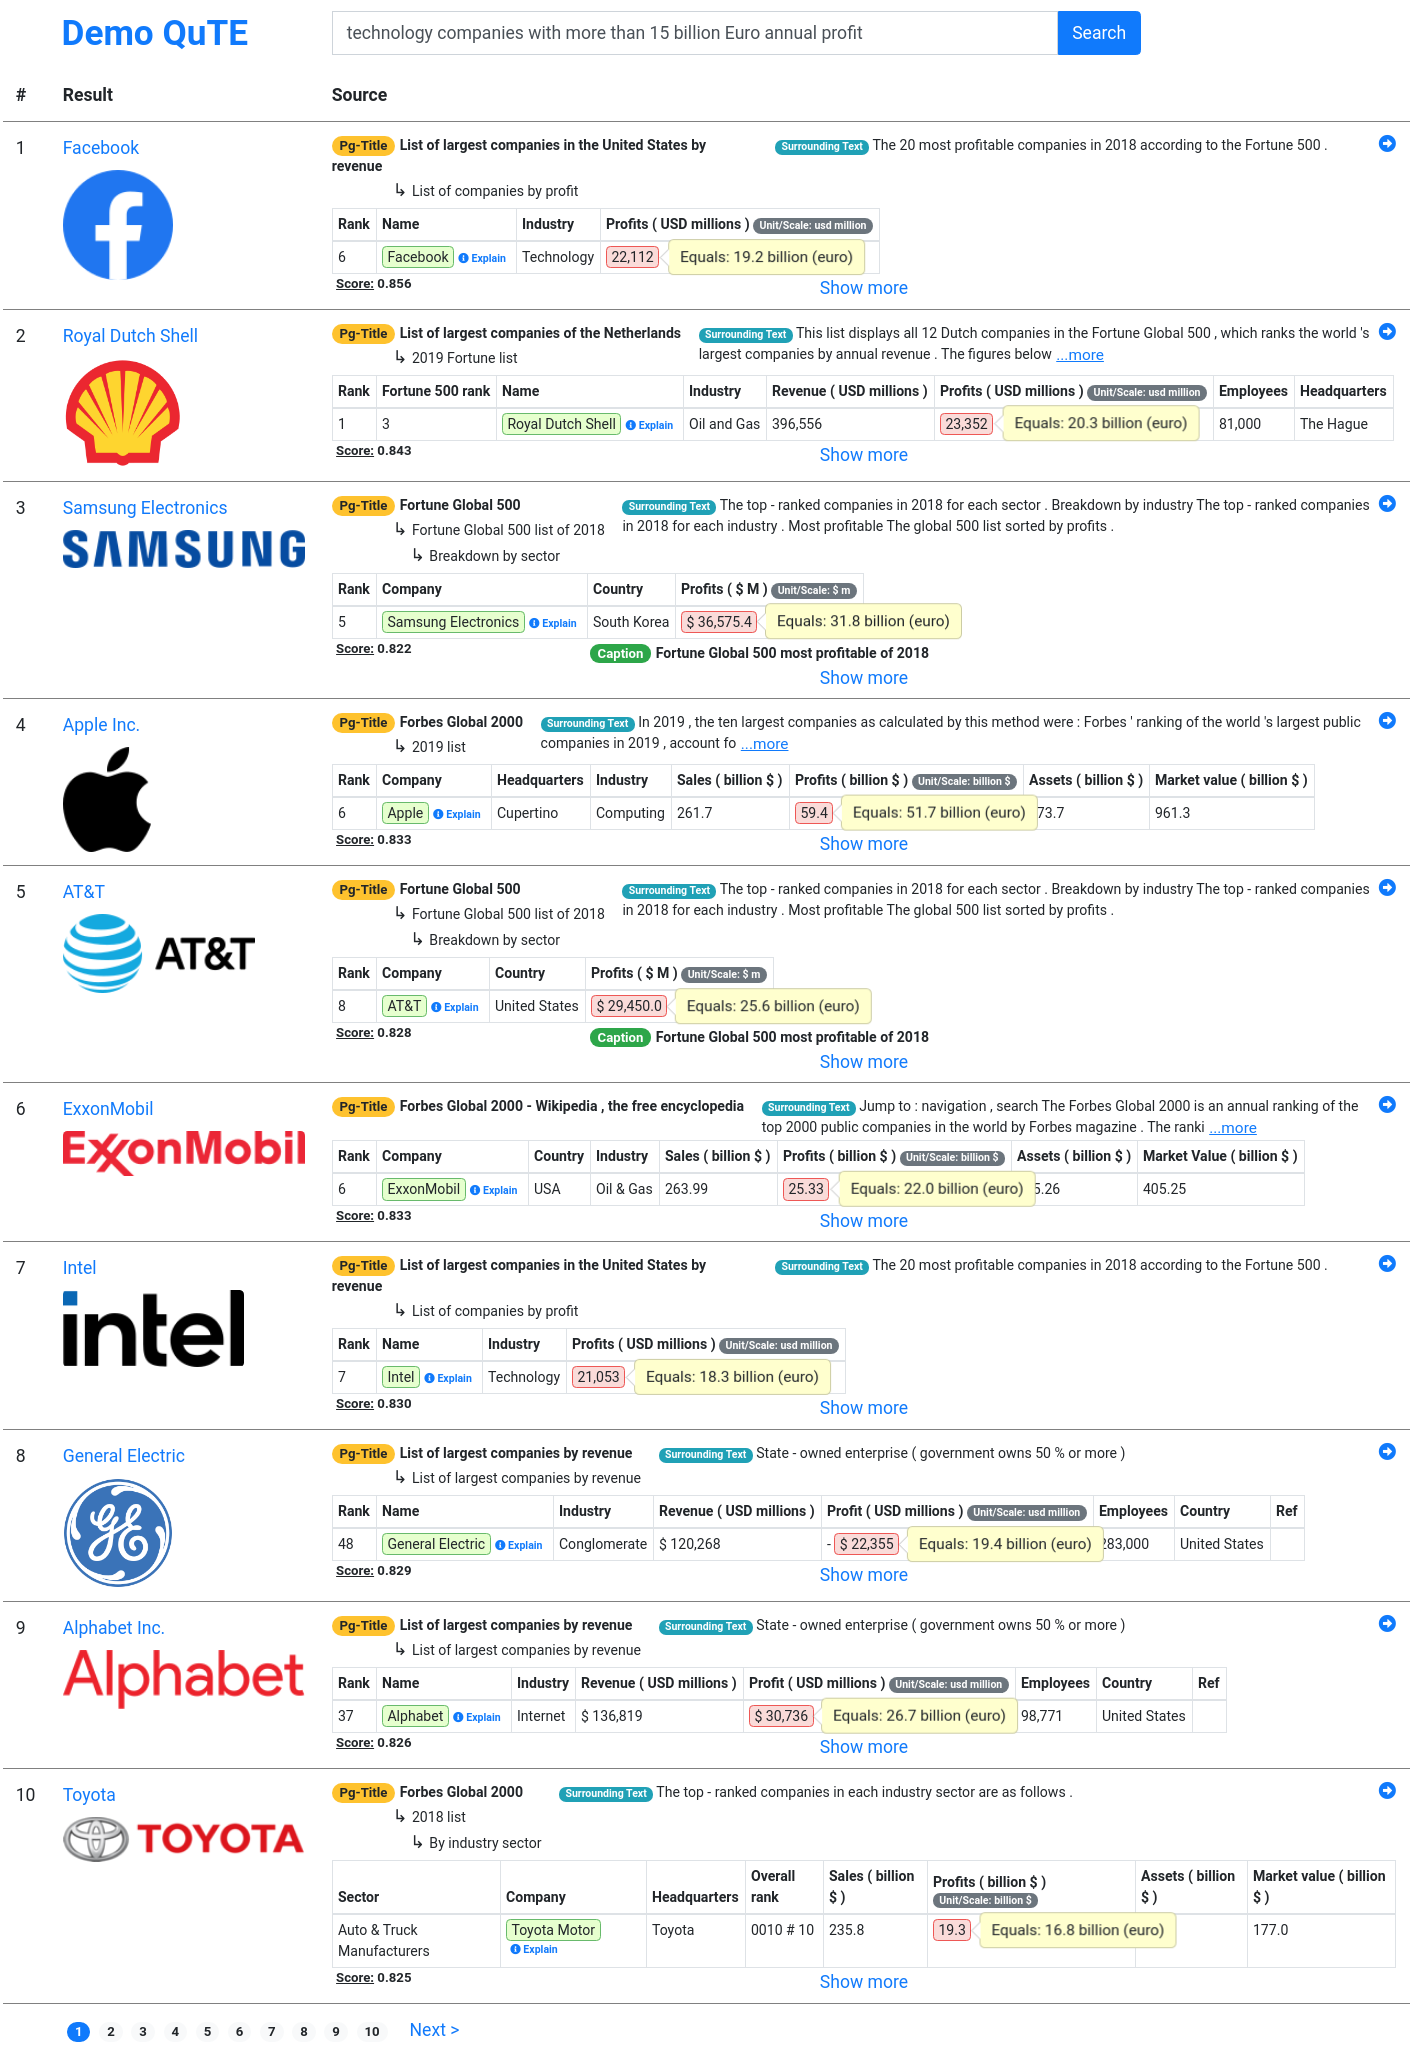
\includegraphics[width=0.7\textwidth]{figures/demo}
% \includegraphics[width=0.75\textwidth]{figures/Qsearch-tables-architecture-11aug2020.pdf}
% \vspace{-0.5em}
\caption{Demo interface of the QuTE-based search system.}
%  \vspace{-0.5em}
\label{fig:demo}
\end{figure}
\twocolumn



\end{document}
\endinput
%%
%% End of file `sample-authordraft.tex'.
